\documentclass{osudissert96}

\usepackage{graphicx,psfrag,amsfonts,float,mathbbol,xcolor,cleveref}
\usepackage{arydshln}
\usepackage{amsmath}
\usepackage{tikz}
\usepackage[mathscr]{euscript}
\usepackage{enumitem}
\usepackage{accents}
\usepackage{framed}
\usepackage[utf8]{inputenc}
\usepackage{natbib}
\usepackage{subcaption}
%\usepackage{subfig}
\usepackage{algorithm}
\usepackage{etoolbox}
\usepackage{lscape}
\usepackage{algorithmic}
\usepackage{nomencl}
\usepackage{natbib}
\usepackage{mathtools}
\usepackage{IEEEtrantools}
\usepackage{times}
\usepackage{arydshln}
\usepackage{amsthm}
\usepackage{booktabs}
\usepackage{rotating}
\usepackage{algorithm}
\usepackage{lscape}

\usepackage[letterpaper, left=1in, top=1in, right=1in, bottom=1in,nohead,includefoot, verbose, ignoremp]{geometry}
\newcommand\numberthis{\addtocounter{equation}{1}\tag{\theequation}}
\newcommand*\needsparaphrased{\color{red}}
\newcommand*\needscited{\color{orange}}
\newcommand*\needsproof{\color{blue}}
\newcommand*\outlineskeleton{\color{green}}
\newcommand{\ms}{\scriptscriptstyle}
\newcommand{\hilbert}{\mathcal{H}}
\newcommand{\hilbertl}{\mathcal{H}_{\langle l \rangle}}
\newcommand{\hilbertm}{\mathcal{H}_{\langle m \rangle}}
\newcommand{\hilbertlnull}{\mathcal{H}_{0\langle l \rangle}}
\newcommand{\hilbertmnull}{\mathcal{H}_{0\langle m \rangle}}
\newcommand{\hilbertlpen}{\mathcal{H}_{1\langle l \rangle}}
\newcommand{\hilbertmpen}{\mathcal{H}_{1\langle m \rangle}}
\newcommand{\PP}{\mathcal{P}}
\newcommand{\vphistar}{\mbox{\boldmath $\phi$}}
\newcommand{\vsigmasq}{\mbox{\boldmath $\sigma^2$}}
\newcommand{\bfeps}{\mbox{\boldmath $\epsilon$}}
\newcommand{\bfgamma}{\mbox{\boldmath $\gamma$}}
\newcommand{\bflam}{\mbox{\boldmath $\lambda$}}
\newcommand{\bfphi}{\mbox{\boldmath $\phi$}}
\newcommand{\bfsigma}{\mbox{\boldmath $\sigma$}}
\newcommand{\bfkappa}{\mbox{\boldmath $\kappa$}}
\newcommand{\bfbeta}{\mbox{\boldmath $\beta$}}
\newcommand{\bfalpha}{\mbox{\boldmath $\alpha$}}
\newcommand{\bftheta}{\mbox{\boldmath $\theta$}}
\newcommand{\bfe}{\mbox{\boldmath $e$}}
\newcommand{\bft}{\mbox{\boldmath $t$}}
\newcommand{\bfg}{\mbox{\boldmath $g$}}
\newcommand{\bfv}{\mbox{\boldmath $v$}}
\newcommand{\bff}{\mbox{\boldmath $f$}}
\newcommand{\bfone}{\mbox{\boldmath $1$}}
\newcommand{\bfo}{\mbox{\boldmath $0$}}
\newcommand{\bfO}{\mbox{\boldmath $O$}}
\newcommand{\bfx}{\mbox{\boldmath $x$}}
\newcommand{\bfX}{\mbox{\boldmath $X$}}
\newcommand{\bfz}{\mbox{\boldmath $z$}}
\newcommand{\tildeY}{\tilde{Y}}
\newcommand{\tildey}{\tilde{y}}
\newcommand{\tildeQ}{\tilde{Q}}
\newcommand{\tildeR}{\tilde{R}}
\newcommand{\tildeA}{\tilde{A}}
\newcommand{\tildeepsilon}{\tilde{\epsilon}}
\newcommand{\bfepsilon}{\mbox{\boldmath $\epsilon$}}
\newcommand{\tildeS}{\tilde{S}}

\newcommand{\bfm}{\mbox{\boldmath $m}}
\newcommand{\bfy}{\mbox{\boldmath $y$}}
\newcommand{\bfa}{\mbox{\boldmath $a$}}
\newcommand{\bfb}{\mbox{\boldmath $b$}}
\newcommand{\bfY}{\mbox{\boldmath $Y$}}
\newcommand{\bfB}{\mbox{\boldmath $B$}}
\newcommand{\bfZ}{\mbox{\boldmath $Z$}}
\newcommand{\tildeB}{\tilde{B}}

\newcommand{\cardT}{\vert \mathcal{T} \vert}
%\newenvironment{theorem}[1][Theorem]{\begin{trivlist}
%\item[\hskip \labelsep {\bfseries #1}]}{\end{trivlist}}
%\newenvironment{corollary}[1][Corollary]{\begin{trivlist}
%\item[\hskip \labelsep {\bfseries #1}]}{\end{trivlist}}
%\newenvironment{proposition}[1][Proposition]{\begin{trivlist}
%\item[\hskip \labelsep {\bfseries #1}]}{\end{trivlist}}
%\newenvironment{definition}[1][Definition]{\begin{trivlist}
%\item[\hskip \labelsep {\bfseries #1}]}{\end{trivlist}}
\newcommand{\argmin}[1]{\underset{#1}{\operatorname{arg}\,\operatorname{min}}\;}
\newtheorem{theorem}{Theorem}[section]
\newtheorem{lemma}[theorem]{Lemma}
\newtheorem{proposition}[theorem]{Proposition}
\newtheorem{corollary}[theorem]{Corollary}

\theoremstyle{definition}
\newtheorem{definition}{Definition}[section]
\newtheorem{example}{Example}[section]
\def\bL{\mathbf{L}}

\begingroup\lccode`~=`_
\lowercase{\endgroup\def~}#1{_{\scriptscriptstyle#1}}
\AtBeginDocument{\mathcode`_="8000 \catcode`_=12 }
\DeclareMathAlphabet{\mathpzc}{OT1}{pzc}{m}{it}

\makeatletter
\renewcommand{\theenumi}{\Roman{enumi}}
\renewcommand{\labelenumi}{\theenumi.}
\renewcommand{\theenumii}{\Alph{enumii}}
\renewcommand{\labelenumii}{\theenumii.}
\renewcommand{\p@enumii}{\theenumi.}
\makeatother


% BibTeX from the BiBTeX Documentation
\def\BibTeX{{\rm B\kern-.05em{\sc i\kern-.025em b}\kern-.08em
    T\kern-.1667em\lower.7ex\hbox{E}\kern-.125emX}}

\renewcommand\typesetChapterTitle[1]{#1}

\begin{document}
\bibliographystyle{plainnat}
%
% First, declare the parts of your title page 
%

\author{Tayler A. Blake}
\title{Nonparametric Covariance Estimation for Longitudinal Data via Tensor Product Splines}
\authordegrees{B.A., M.S.}  % Degrees thus far, not including this one.
\unit{Department of Statistics}

\advisorname{Yoonkyung Lee}
\member{Katherine A. Calder}
\member{Sebastian Kurtek}
%\member{Yet another dude}      % Normally you will have advisor + 2 members

\maketitle

% Next, EITHER a copyright or BLANK page.
%
%   The following creates a page used to copyright your dissertation
%
%   BACKGROUND: Even without this copyright page, your dissertation will
%               carry a common-law copyright. However, if your
%               dissertation ends up seeing wide distribution, your
%               common-law copyright is at risk of being expunged.
%               Adding this copyright page prevents that from happening.
%
%               There are NO DOWNSIDES to including a copyright page as
%               your document is automatically copyright by law anyway.
%               However, this copyright page is OPTIONAL. If you get rid
%               of it, uncomment the \blankpage that follows it so that
%               there is a blank page here. The graduate school requires
%               a page here that is either blank or carries the
%               copyright.
%
%   IMPORTANT NOTE: The graduate school requires either a copyright page
%                   here or a BLANK PAGE here. If you get rid of the
%                   copyright, uncomment the \blankpage that follows it.
%                   You should NOT have BOTH uncommented.
%

% If you get rid of \disscopyright, restore the \blankpage line after it
\disscopyright
%\blankpage

%
% Abstract goes here.
%

\begin{abstract}
  %  The dissertation abstract can only be 500 words.


\begin{quote}
%
%With high dimensional longitudinal and functional data becoming much more common, there is a strong need for methods of estimating large covariance matrices. Estimation is made difficult by the instability of sample covariance matrices in high dimensions and a positive- definite constraint we desire to impose on estimates. A Cholesky decomposition of the covariance matrix allows for parameter estimation via unconstrained optimization as well as a statistically meaningful interpretation of the parameter estimates. Regularization improves stability of covariance estimates in high dimensions, as well as in the case where functional data are sparse and individual curves are sampled at different and possibly unequally spaced time points. By viewing the entries of the covariance matrix as the evaluation of a continuous bivariate function at the pairs of observed time points, we treat covariance estimation as bivariate smoothing.
%Within regularization framework, we propose novel covariance penalties which are designed to yield natural null models presented in the literature for stationarity or short-term dependence. These penalties are expressed in terms of variation in continuous time lag and its orthogonal complement. We present numerical results and data analysis to illustrate the utility of the proposed method.
%
%\bigskip

Estimation of an unstructured covariance matrix is difficult because of the challenges posed by parameter space dimensionality and the positive definiteness constraint that estimates should satisfy. We propose a general framework for nonparametric covariance estimation when the variables have a natural ordering. Modeling the Cholesky decomposition of the covariance matrix removes any constraints from estimation, including those posed by positiveness definiteness. In addition, the Cholesky decomposition enjoys the added advantage over alternative matrix decompositions of supplying a meaningful statistical interpretation of the corresponding estimated parameters. We illustrate the equivalence of covariance estimation and the estimation of a varying coefficient autoregressive model. By defining the varying coefficient as a bivariate function, we naturally accommodate sparsely or irregularly sampled longitudinal data without the need for imputation methods. 

\bigskip

This framework extends the set of tools available for covariance estimation to any of those employed in the typical function estimation setting. Viewing stationarity as a form of simplicity or parsimony in covariance models, we specify the varying coefficient as a function so that we can conveniently penalize the components capturing the nonstationarity in the fitted function. We demonstrate covariance estimation as a bivariate smoothing problem estimation through the construction of the estimator using the smoothing spline framework of \cite{kimeldorf1971some}, as well the P-splines of \cite{eilers1996flexible} . A simulation study establishes the advantage of our estimator over alternative estimators proposed in this setting. We analyze a longitudinal dataset to illustrate application of the methodology and compare our estimates to those resulting from alternative models proposed for the covariance for longitudinal data. 

\end{quote}



\end{abstract}


%
% UPDATED TEXT (2010):
%  The graduate school does not require an external abstract. If this
%  changes, follow the old instructions below.
%
% HISTORICAL TEXT (1996):
%  Uncomment the three lines below to generate the external abstract.  Two
%  copies of this must be turned in to the graduate school.  These lines can
%  be placed pretty much anywhere, since the page numbering should be
%  independent of the rest of the thesis
%

% \begin{externalabstract}
%   %  The dissertation abstract can only be 500 words.


\begin{quote}
%
%With high dimensional longitudinal and functional data becoming much more common, there is a strong need for methods of estimating large covariance matrices. Estimation is made difficult by the instability of sample covariance matrices in high dimensions and a positive- definite constraint we desire to impose on estimates. A Cholesky decomposition of the covariance matrix allows for parameter estimation via unconstrained optimization as well as a statistically meaningful interpretation of the parameter estimates. Regularization improves stability of covariance estimates in high dimensions, as well as in the case where functional data are sparse and individual curves are sampled at different and possibly unequally spaced time points. By viewing the entries of the covariance matrix as the evaluation of a continuous bivariate function at the pairs of observed time points, we treat covariance estimation as bivariate smoothing.
%Within regularization framework, we propose novel covariance penalties which are designed to yield natural null models presented in the literature for stationarity or short-term dependence. These penalties are expressed in terms of variation in continuous time lag and its orthogonal complement. We present numerical results and data analysis to illustrate the utility of the proposed method.
%
%\bigskip

Estimation of an unstructured covariance matrix is difficult because of the challenges posed by parameter space dimensionality and the positive definiteness constraint that estimates should satisfy. We propose a general framework for nonparametric covariance estimation when the variables have a natural ordering. Modeling the Cholesky decomposition of the covariance matrix removes any constraints from estimation, including those posed by positiveness definiteness. In addition, the Cholesky decomposition enjoys the added advantage over alternative matrix decompositions of supplying a meaningful statistical interpretation of the corresponding estimated parameters. We illustrate the equivalence of covariance estimation and the estimation of a varying coefficient autoregressive model. By defining the varying coefficient as a bivariate function, we naturally accommodate sparsely or irregularly sampled longitudinal data without the need for imputation methods. 

\bigskip

This framework extends the set of tools available for covariance estimation to any of those employed in the typical function estimation setting. Viewing stationarity as a form of simplicity or parsimony in covariance models, we specify the varying coefficient as a function so that we can conveniently penalize the components capturing the nonstationarity in the fitted function. We demonstrate covariance estimation as a bivariate smoothing problem estimation through the construction of the estimator using the smoothing spline framework of \cite{kimeldorf1971some}, as well the P-splines of \cite{eilers1996flexible} . A simulation study establishes the advantage of our estimator over alternative estimators proposed in this setting. We analyze a longitudinal dataset to illustrate application of the methodology and compare our estimates to those resulting from alternative models proposed for the covariance for longitudinal data. 

\end{quote}



% \end{externalabstract}

%
%  My Dedication
%

\dedication{This is dedicated to the one I love \ldots\ la la la \ldots}


%
% Bring in Acknowledgement and Vita from separate files named ``ack.tex''
% and ``vita.tex''.
%

\begin{acknowledgements}
I thank everyone who has ever had a cow. \ldots

In reality, this is the only page of the dissertation which the author
has full control of. You can write anything you want here, and no one
can tell you it's wrong (except if the margins don't line up!!!!).
\end{acknowledgements}


\begin{vita}



\dateitem{May 2007}{B.S. Mathematics and Computer Science,\\
				Capital University,\\
				Columbus, OH}
\dateitem{May 2007}{Winner, James L. and E. Marlene Bruning Award for Undergraduate Research,\\
				Capital University,\\
				Columbus, OH}

\dateitem{December 2009}{M.S. Statistics,\\
					The Ohio State University,\\
					Columbus, OH}

\dateitem{May 2014 - December 2015}{Data Scientist,\\
			 Starbucks Coffee Co.\\
			 Seattle, WA}

\dateitem{January 2016 - December 2016}{Machine Learning Engineer,\\
			 Pillar Technology Inc.\\
			 Columbus, OH}

\dateitem{January 2017 - present}{Senior Data Scientist,\\
			 Information Control Company,\\
			 Columbus, OH}


\begin{fieldsstudy}
\majorfield{Statistics}
\end{fieldsstudy}
%% UPDATE FOR 2010:
%  Grad school only wants research publications, and it only wants those
%  research pubs that are actually published. Accepted or ``to appear''
%  publications don't count. If they look closely, they'll tell you to
%  remove any publications that aren't in print. Haivng said that, they
%  probably won't look that closely unless you put a really long list
%  here. You're tempting fate if you add instructional publications
%  though.

\end{vita}




%
% Make the Table of Contents and other good stuff
%

\tableofcontents
\listoftables
\listoffigures


%
% The following is a list of chapters.  Each is brought in from a
% separate file using the \include{} command.
%


An estimate of the covariance matrix or its inverse is required for nearly all statistical procedures in classical multivariate data analysis, time series analysis, spatial statistics and, more recently, the growing field of statistical learning. Covariance estimates play a critical role in the performance of techniques for clustering and classification such as linear discriminant analysis (LDA), quadratic discriminant analysis (QDA), factor analysis, and principal components analysis (PCA), analysis of conditional independence through graphical models, classical multivariate regression, prediction, and Kriging. Covariance estimation with high dimensional data has has recently gained growing interest; it is generally recognized that there are two primary hurdles responsible for the difficulty in covariance estimation: the instability of sample covariance matrices in high dimensions and a positive-definite constraint we wish estimates to obey.

\bigskip

Prevalent technological advances in industry and many areas of science make high dimensional longitudinal and functional data a common occurrence, arising in numerous areas including medicine, public health, biology, and environmental science with specific applications including fMRI, spectroscopic imaging, gene microarrays among many others, presenting a need for effective covariance estimation in the challenging situation where parameter dimensionality $p$ is possibly much larger than the number of observations, $n$. 

\bigskip

We consider two types of potentially high dimensional data: the first is the case of functional data or times series data, where each observation corresponds to a curve sampled densely at a fine grid of time points; in this case, it is typical that the number of time points is larger than the number of observations. The second is the case of sparse longitudinal data where measurement times may be almost unique yet sparsely distributed within the observed time range for each individual in the study. In this case, the nature of the high dimensionality may not be a consequence of having more measurements per subject than the number of subjects themselves, but rather because when pooled across subjects, the total number of unique observed time points is greater than the number of individuals.  Several approaches have been taken in effort to overcome the issue of high dimensionality in covariance estimation. Regularization improves stability of covariance estimates in high dimensions, particularly in the case where the parameter dimensionality $p$ is much larger than the number of observations $n$. Regularization of the covariance matrix and its Cholesky decomposition has been explored extensively through various approaches including banding, tapering, kernel smoothing, penalized likelihood, and penalized regression; see citet{pourahmadi2011covariance} for a comprehensive overview. 

\bigskip

To overcome the hurdle of enforcing covariance estimates to be positive definite, several have considered modeling various matrix decompositions including variance-correlation decomposition, spectral decomposition, and Cholesky decomposition. The Cholesky decomposition has received particular attention, as it which allows for a statistically meaningful interpretation as well as an unconstrained parameterization of elements of the covariance matrix. This parameterization allows for estimation to be accomplished as simply as in least squares regression. If we assume that the data follow an autoregressive process with (possibly) heteroskedastic errors, then the two matrices comprising the Cholesky decomposition, the Cholesky factor (which diagonalizes the covariance matrix) and diagonal matrix itself, hold the autoregressive coefficients and the error variances, respectively.

\bigskip

In longitudinal studies, the measurement schedule could consist of targeted time points or could consist of completely arbitrary (random) time points. If either the measurement schedule has targeted time points which are not necessarily equally spaced or if there is missing data, then we have what is considered incomplete and unbalanced data. If the measurement schedule has arbitrary or almost unique time points for every individual so that at a given time point there could be very few or even only a single measurement, we must consider how to handle what we consider as sparse longitudinal data. We view the response as a stochastic process with corresponding continuous covariance function and the generalized autoregressive parameters as the evaluation of a continuous bivariate function at the pairs of observed time points rather than specifying a finite set of observations to be multivariate normal and estimating the covariance matrix. This is advantageous because it is unlikely that we are only interested in the covariance between pairs of observed design points, so it is reasonable to approach covariance estimation in a way that allows us to obtain an estimate of the covariance between two measurements at any pair of time points within the time interval of interest. 

\bigskip


Through the Cholesky decomposition, we formulate covariance estimation as a penalized regression problem and propose novel covariance penalties designed to yield natural null models presented in the literature. By transforming the axes of the design points, we express these penalties in terms of two directions: the lag component and the additive component and characterize the solution coefficient function in terms of a functional ANOVA decomposition. Some have side-stepped the issue of high dimensionality by prescribing simple parametric models for the elements of the Cholesky decomposition.  \citet{chen2011efficient}, \citet{pourahmadi1999joint}, and \citet{pourahmadi2002dynamic} have elicited stationary parametric models for the generalized autoregressive coefficients, letting the GARPs depend only on the distance between two time points. To induce the structural simplicity of such stationary models with the flexibility of a nonparametric approach, we penalize all functional components but that corresponding to the lag component so that the set of null models is comprised of stationary models.  \citet{huang2007estimation} follow the hueristic argument presented in \citet{pourahmadi1999joint} that the generalized autoregressive parameters are monotone decreasing in as lag increases and set off-diagonal elements of either the covariance matrix or the Cholesky factor corresponding to large lags to zero. Rather than shrinking element of the Cholesky factor to zero after particular value of $l$, we choose to enforce structure of the Cholesky factor such that the null models coincide with parsimonious models commonly used in time series analysis and with simple parametric models proposed in the nonparametric covariance estimation literature.

\bigskip

The remainder of the chapter serves as a brief survey of developments in covariance estimation.  We will highlight a number of approaches to parsimonious covariance modeling, but our attention will be delegated to recent progress in parsimonious covariance models for longitudinal data. The review will conclude with the presentation of matrix factorizations for reparameterizing elements of the covariance matrix, translating covariance estimation into a generalized linear modeling problem.	
     
\documentclass[12pt]{article}
\usepackage{graphicx,psfrag,amsfonts,float,mathbbol,xcolor,cleveref}
\usepackage{arydshln}
\usepackage{amsmath}
\usepackage{tikz}
\usepackage[mathscr]{euscript}
\usepackage{enumitem}
\usepackage{accents}
\usepackage{framed}
\usepackage{subcaption}
\usepackage{natbib}
\usepackage{mathtools}
\usepackage{IEEEtrantools}
\usepackage{times}
\usepackage{cite}
\usepackage{amsthm}
\usepackage[letterpaper, left=1in, top=1in, right=1in, bottom=1in,nohead,includefoot, verbose, ignoremp]{geometry}
\newcommand{\comment}[1]{\text{\phantom{(#1)}} \tag{#1}}
\newcommand\numberthis{\addtocounter{equation}{1}\tag{\theequation}}
\newcommand*\needsparaphrased{\color{red}}
\newcommand*\needscited{\color{orange}}
\newcommand*\needsproof{\color{blue}}
\newcommand*\outlineskeleton{\color{green}}
\newcommand{\ms}{\scriptscriptstyle}
\newcommand{\PP}{\mathcal{P}}
\newcommand{\vphistar}{\mbox{\boldmath $\phi^*$}}
\newcommand{\vsigmasq}{\mbox{\boldmath $\sigma^2$}}
\newcommand{\bfeps}{\mbox{\boldmath $\epsilon$}}
\newcommand{\bfgamma}{\mbox{\boldmath $\gamma$}}
\newcommand{\bflam}{\mbox{\boldmath $\lambda$}}
\newcommand{\bfphi}{\mbox{\boldmath $\phi$}}
\newcommand{\bfsigma}{\mbox{\boldmath $\sigma$}}
\newcommand{\bfbeta}{\mbox{\boldmath $\beta$}}
\newcommand{\bfalpha}{\mbox{\boldmath $\alpha$}}
\newcommand{\bfe}{\mbox{\boldmath $e$}}
\newcommand{\bff}{\mbox{\boldmath $f$}}
\newcommand{\bfone}{\mbox{\boldmath $1$}}
\newcommand{\bft}{\mbox{\boldmath $t$}}
\newcommand{\bfo}{\mbox{\boldmath $0$}}
\newcommand{\bfO}{\mbox{\boldmath $O$}}
\newcommand{\bfx}{\mbox{\boldmath $x$}}
\newcommand{\bfX}{\mbox{\boldmath $X$}}
\newcommand{\bfz}{\mbox{\boldmath $z$}}


\newcommand{\bfm}{\mbox{\boldmath $m}}
\newcommand{\bfy}{\mbox{\boldmath $y$}}
\newcommand{\bfa}{\mbox{\boldmath $a$}}
\newcommand{\bfb}{\mbox{\boldmath $b$}}
\newcommand{\bfY}{\mbox{\boldmath $Y$}}
\newcommand{\bfS}{\mbox{\boldmath $S$}}
\newcommand{\bfZ}{\mbox{\boldmath $Z$}}
\newcommand{\cardT}{\vert \mathcal{T} \vert}
%\newenvironment{theorem}[1][Theorem]{\begin{trivlist}
%\item[\hskip \labelsep {\bfseries #1}]}{\end{trivlist}}
%\newenvironment{corollary}[1][Corollary]{\begin{trivlist}
%\item[\hskip \labelsep {\bfseries #1}]}{\end{trivlist}}
%\newenvironment{proposition}[1][Proposition]{\begin{trivlist}
%\item[\hskip \labelsep {\bfseries #1}]}{\end{trivlist}}
%\newenvironment{definition}[1][Definition]{\begin{trivlist}
%\item[\hskip \labelsep {\bfseries #1}]}{\end{trivlist}}

\newtheorem{theorem}{Theorem}[section]
\newtheorem{lemma}[theorem]{Lemma}
\newtheorem{proposition}[theorem]{Proposition}
\newtheorem{corollary}[theorem]{Corollary}

\theoremstyle{definition}
\newtheorem{definition}{Definition}[section]
\newtheorem{example}{Example}[section]
\def\bL{\mathbf{L}}

\begingroup\lccode`~=`_
\lowercase{\endgroup\def~}#1{_{\scriptscriptstyle#1}}
\AtBeginDocument{\mathcode`_="8000 \catcode`_=12 }

\makeatletter
\renewcommand{\theenumi}{\Roman{enumi}}
\renewcommand{\labelenumi}{\theenumi.}
\renewcommand{\theenumii}{\Alph{enumii}}
\renewcommand{\labelenumii}{\theenumii.}
\renewcommand{\p@enumii}{\theenumi.}
\makeatother

\begin{document}

%\nocite{*}
\def\bL{\mathbf{L}}
%\usepackage{mathtime}

%%UNCOMMENT following line if you have package


\title{ Nonparametric Covariance Estimation for Longitudinal Data via Penalized Tensor Product Splines}

\author{Tayler A. Blake\thanks{The Ohio State University, 1958 Neil Avenue, Columbus, OH 43201} \and  Yoonkyung Lee\thanks{The Ohio State University, 1958 Neil Avenue, Columbus, OH 43201}}

\bibliographystyle{plainnat}
\maketitle

\section{Smoothing Spline Varying-coefficient Models for Covariance Estimation}

A predominant difficulty in the estimation of covariance matrices is the potentially high dimensionality of the problem, as the number of unknown elements in the covariance matrix grows quadratically with the size of the matrix. It is well-known that the sample covariance matrix can be unstable in high dimensions; ways for controlling the complexity of estimates is highly desirable for improving stability of estimates. In the longitudinal-data literature, it is a common practice to use parametric models for the covariance structure.  Many have specified parsimonious parametric models for $\phi_{ijk}$ to overcome the issue of dimensionality.   A commonly utilized approach in previous work is to model $\phi_{ijk} = z_{ijk}^T \gamma$ where $z_{ijk}$ is a vector of powers of time differences and $\gamma$ is a vector of unknown ``dependence'' parameters to be estimated from the data. \citet{chen2011efficient}, \citet{lin2009robust}, \citet{pan2003modelling},  and \citet{pourahmadi1999joint} define

\begin{equation}
z_{ijk}^T = \left(1, t_{ij} - t_{ik},\left( t_{ij} - t_{ik} \right)^2, \dots, \left(t_{ij} - t_{ik}\right)^{q-1} \right) \label{covmodel}
\end{equation}

Modeling the covariance in such a way is reduces a potentially high dimensional problem to something much more computationally feasible; if one models the innovation variances $\sigma^2\left(t\right)$ similarly using a $d$-dimensional vector of covariates, the problem reduces to estimating $q+d$ unconstrained parameters, where much of the dimensionality reduction is a result of characterizing the GARPs in terms of only the difference between pairs of observed time points, and not the time points themselves.  Modeling $\phi$ in such a way is equivalent to specifying a Toeplitz structure for $\Sigma$. A $p \times p$ Toeplitz matrix $M$ is a matrix with elements $m_{ij}$ such that $m_{ij} = m_{\vert i-j \vert}$ i.e. a matrix of the form

\begin{equation}
M = \begin{bmatrix} m_0 & m_1 & m_2 & \dots & m_{p-1}\\ m_1 & m_0 & m_1 & \dots & m_{p-2}\\m_2 & m_1 & m_0 & \dots & m_{p-3}\\ \vdots & \vdots & \vdots & \ddots & \vdots\\  m_{p-1} & m_{p-2} & m_{p-3} & \dots & m_0 \end{bmatrix} \label{toeplitz}
\end{equation}

\bigskip

The estimated covariance matrix may be considerably biased when the specified parametric model is far from the truth.  To avoid model misspecification that potentially accompanies parametric analysis, many have alternatively  proposed nonparametric and semiparametric techniques approaches to estimation.  While these estimators can be very flexible and thus exhibit low bias, this advantage can be offset with high variance.  To balance the tradeoff between bias and variance, shrinkage or regularization may be applied to estimates to improve stability of estimators. \citet{diggle1998nonparametric} proposed nonparametric estimation of the covariance matrix of longitudinal data by smoothing raw sample variogram ordinates and squared residuals.  [DISCUSS THE NONPARAMETRIC SMOOTHER OF HANS GEORG MULLER HERE]  However, neither of these methods ensure that the resulting estimates are positive-definite.  

\bigskip
Several others have proposed methods for covariance estimation within the same paradigm of a smooth, continuous function underlying a discretized covariance matrix associated with the observed data. 
\citet{pourahmadi1999joint} employ the Cholesky decomposition to guarantee positive-definiteness and imposed structure on the elements of the Cholesky decomposition and heuristically argue that $\phi_{t,t-l}$ should be monotonically decreasing in $l$. That is, the effect of $y_{t-l}$ on $y_t$ through the autoregressive parameterization should decrease as the distance in time between the two measurements increases. In similar spirit, others including \citet{bickel2008regularized} and \citet{levina2008sparse} enforce such structure by setting $\phi_{t,t-l}$ equal to zero for $l$ large enough, or equivalently, setting all subdiagonals of $T$ to zero beyond the $K^{th}$ off-diagonal. The tuning parameter $K$ is chosen using a model selection criterion such as Akaike information criterion, Bayesian information criterion, or cross validation or a variant thereof.  In terms of the autoregressive model corresponding to the Cholesky decomposition, this form of regularization, known as ``banding'' the Cholesky factor $T$, is equivalent to regressing $y_t$ on only its $K$ immediate predecessors, setting $\phi_{tj} = 0$ for $t-j>K$. 

\bigskip

From this perspective, it is apparent that the presentation of covariance estimation as a least squares regression problem suggests that the familiar ideas of model regularization for least-squares regression can be used for estimating covariances.  Wu and Pourahmadi \citet{wu2003nonparametric} proposed a two-step estimation procedure using nonparametric smoothing for regularized estimation of large covariance matrices.  In the first step, they derive a raw estimate of the covariance matrix and the estimated covariance matrix is subject to the modified Cholesky decomposition. In the second step, they apply local polynomial smoothing to the diagonal elements of $D$ and the subdiagonals of $T$. The use of the Cholesky parameterization guarantees that their estimate is guaranteed to be positive-definite, however, their procedure is not capable of handling missing data. \citet{huang2007estimation} 

however, their two-step method did not utilize the information that many of the subdiagonals of T are essentially zeros at the first step. Inefficient estimation may result because of ignoring regularization structure in constructing the raw estimator. 

Several have applied these approaches to covariance estimation; \citet{huang2007estimation} jointly model the mean and covariance matrix of longitudinal data using basis function expansions. They employ the Cholesky decomposition of the covariance matrix and treat the subdiagonals of $T$ as smooth functions, approximated by B-splines. Estimation is carried out by maximizing the normal likelihood. Their method permits subject-specific observations times, but assumes that observation times lie on some notion of a regular grid. They treat within-subject gaps in measurements as missing data and which they handle using the E-M algorithm. 

\bigskip

We naturally accommodate irregularly spaced data and unequal sample sizes between subjects by defining the autoregressive parameters as the values of a smooth function evaluated at within-subject pairs of observed time points.  Furthermore, by viewing $\phi\left(t,s\right)$ as a smooth \emph{bivariate} function, we can utilize the information across the subdiagonals of $T$ to inform the fit, rather than treating each subdiagonal separately.  As in the classical nonparametric function estimation setting, we assume $\phi$ to vary in a high-dimensional (possibly infinite) function space. We propose two representations of $\phi\left(\cdot, \cdot\right)$ and $\sigma\left(\cdot, \cdot\right)$: approximation by smoothing splines and approximation by B-spline basis expansion. 

\subsection{Smoothing spline representation of $\phi$, $\sigma$}

Let $\mathcal{H} = \mathcal{H}_{0} \oplus \mathcal{H}_{1}$ be the reproducing kernel Hilbert space (r.k.h.s) corresponding to the tensor product of the first-order and second-order Sobolev spaces:

\[
\mathcal{H} = \mathcal{H}_{l} \otimes \mathcal{H}_{m}, \;\; \mathcal{H}_{l} = W_2\left(0,1\right),\;\;\mathcal{H}_{m} = W_1\left(0,1\right)\;\mbox{where }
\]

\[W_m\left(0,1\right) \equiv \lbrace f: \;\;f^\prime, \dots, f^{\left( m-1 \right)} \mbox{absolutely continuous}, \int_0^1 \left(f^{\left( m \right)}\right)^2 dt < \infty \rbrace\]
\noindent
We seek $\phi^*\left(\cdot, \cdot \right) \in \mathcal{H}$ which minimizes
\begin{equation}
\frac{1}{2}\sum_{i=1}^N \sum_{j=2}^{n_i} {\sigma^{-2}_{ij}}\left( y\left(t_{ij}\right) - \sum_{k=1}^{n_i - 1}\phi^*\left(l^i_{jk},m^i_{jk} \right)y\left(t_{ik}\right) \right)^2 + \lambda J\left(\phi^*\right)  
\label{eq:objectivefun}
\end{equation}
\noindent
where $P_1 \phi^*$ is the projection of $\phi^*$ onto $\mathcal{H}_1$, $J\left(\phi^*\right) = \vert \vert P_1 \phi^* \vert \vert^2$. Define the differential operator $M_\nu f = \int_0^1 f^{\left( m \right)}\left(x\right) dx\;,\;\; \nu = 1, \dots, m$ and endow $W_m\left(0,1\right)$ with inner product
%\begin{equation}
%\left< f,g\right> = \underbrace{\sum_{\nu=0}^{m-1} M_\nu f M_\nu g}_{\left< f,g\right>_0} + \underbrace{\int_0^1 f^{\left( m \right)}\left(x\right)g^{\left( m \right)}\left(x\right)dx}_{\left< f,g\right>_1}
%\end{equation}

\begin{equation}
\left< f,g\right> = \left< f,g\right>_0 + \left< f,g\right>_1 = \sum_{\nu=0}^{m-1} M_\nu f M_\nu g + \int_0^1 f^{\left( m \right)}\left(x\right)g^{\left( m \right)}\left(x\right)dx
\end{equation}
\noindent
which induces norm 
\[
\vert \vert f \vert \vert^2 = \left< f,f\right> = \left< f,f\right>_0 + \left< f,f\right>_1 = \vert \vert P_0 f \vert \vert^2 + \vert \vert P_1 f \vert \vert^2
\]
\noindent
Let $k_j\left(x\right) = B_j\left(x\right)/{j!}$ for $x \in \left[0,1\right]$, where $B_j\left(x\right)$ is the $j^{th}$ Bernoulli polynomial which can be defined according to the recursive relationship:

\[
B_0\left(x\right) = 1,\;\;\;\;\;\; \frac{d}{dx} B_r\left(x\right) = rB_{r-1}\left(x\right)
\]
\noindent
Noting that $M_\nu B_r = \delta_{\nu-r}$, $W_m$ can be written as a direct sum of the $m$ orthogonal subspaces: $\lbrace k_r \rbrace_{r=0}^{m-1}$ and $W_m^1$.   Here, $\lbrace k_r \rbrace$ is the subspace spanned by $k_r$ and $W_m^1$ is the space orthogonal to $W_m^0 \equiv \lbrace 1 \rbrace \oplus \lbrace k_1 \rbrace \oplus \dots \oplus \lbrace k_{m-1} \rbrace$ which satisfies 
\[
W_m^1 = \lbrace f: M_\nu f = 0,\;\; \nu = 0,1,\dots, m-1\rbrace
\]

\noindent
Writing $\mathcal{H}$ as the tensor product of the two decomposed Sobolev spaces, we have

\begin{eqnarray}
\mathcal{H} = \mathcal{H}_l  \otimes \mathcal{H}_m &=& W_2 \otimes W_1 \label{eq:HilbertDecomp} \\ 
&=& \left[ W_2^0 \oplus W_2^1 \right] \otimes \left[ W_1^0 \oplus W_1^1 \right] \nonumber \\ 
&=& \left[ \left[ \lbrace 1 \rbrace \oplus \lbrace k_1 \rbrace \right] \oplus W_2^1 \right] \otimes \left[ \lbrace 1 \rbrace \oplus W_1^1 \right] \nonumber \\ 
&=&\left[ \lbrace 1 \rbrace  \oplus \lbrace k_1 \rbrace \right] \oplus W_2^1 \oplus W_1^1 \oplus  \left[ \lbrace k_1 \rbrace  \otimes  W_1^1 \right]  \oplus  \left[W_2^1 \otimes  W_1^1   \right] \nonumber \\
&\equiv& \left[ \mathcal{H}_{\mu^*} \oplus \mathcal{H}_l^0 \right] \oplus \left[ \mathcal{H}_l^1 \oplus \mathcal{H}_m^1 \oplus \mathcal{H}_{lm}^{01} \oplus \mathcal{H}_{lm}^{11}\right]
\nonumber\\
&=& \mathcal{H}_0 \oplus \mathcal{H}_1
\nonumber
\end{eqnarray} 

\noindent
where the functional components corresponding to $\mathcal{H}_\mu$, $\mathcal{H}_l^0$, $\mathcal{H}_l^1$, $\mathcal{H}_m^1$, and $\left[ \mathcal{H}_{lm}^{01} \oplus \mathcal{H}_{lm}^{11}\right]$ are the overall mean, the nonparametric main effect of $l$, the parametric main effect of $l$, the parametric main effect of $m$, the nonparametric-parametric interaction, and the parametric-parametric interaction (between $l$ and $m$). Given this decomposition of the function space, any $\phi^* \in \mathcal{H}$ may be written as a sum of components from each of the 

\begin{equation}
\phi^*\left(l,m\right) = \mu^* + \phi_l^*\left(l\right) + \phi_m^*\left(m\right) + \phi_{lm}^*\left(l,m\right)  \label{eq:ANOVAdecomp}
\end{equation} 
\noindent
where $\int_{0}^1 \phi^*_{l}\left(l\right)dl = \int_{0}^1 \phi^*_{m}\left(m\right)dm = 0$, $\int_{0}^1 \phi^*_{lm}\left(l,m\right)dl = \int_{0}^1 \phi^*_{lm}\left(l,m\right)dm = 0$. The reproducing kernel (r.k.) for $\lbrace k_r \rbrace$ is $k_r\left(x \right)k_r\left(x^\prime \right)$. It can be verified that the r.k. for $W_m^1$ (Craven and Wahba 1979) is given by $R^1\left(x,x^\prime\right) = k_m\left(x \right)k_m\left(x^\prime \right) + \left( -1 \right)^{m-1}k_{2m}\left(\left[ x-x^\prime \right] \right)$
where $\left[ \alpha \right]$ is the fractional part of $\alpha$. The r.k. for $W_m$ is given by 
\begin{eqnarray*}
R\left(x,x^\prime\right) &=& R^0\left(x,x^\prime\right) + R^1\left(x,x^\prime\right) \\
&=&\left[ \sum_{\nu=1}^{m-1} k_\nu\left(x \right)k_\nu\left(x^\prime \right) \right]+ \left[ k_m\left(x \right)k_m\left(x^\prime \right) + \left( -1 \right)^{m-1}k_{2m}\left(\left[ x-x^\prime \right] \right)\right] \label{eq:RKforH1}
\end{eqnarray*}
\noindent
Using the fact that the r.k. for a tensor product space is the product of the corresponding reproducing kernels, the r.k. for $\mathcal{H}$ is given by 
\begin{eqnarray}
R\left( \left(l,m\right),\left(l^\prime,m^\prime\right)\right) &=&  R_l\left(l,l^\prime\right) \times R_m\left(m,m^\prime\right) \nonumber \\
 &=& \left[  R_l^0\left(l,l^\prime\right) + R_l^1\left(l,l^\prime\right) \right] \times \left[  R_m^0\left(l,l^\prime\right) + R_m^1\left(l,l^\prime\right) \right] \nonumber \\
 &=& R_l^0\left(l,l^\prime\right)R_m^0\left(m,m^\prime\right) + R_l^0\left(l,l^\prime\right) R_m^1\left(m,m^\prime\right) \nonumber \\
&\mbox{ }&\;\;\;\;\;\;\;\;\;\;\;\;\;\;\;\;\;\;\;\;\;\;\;\;\;\;\;\;\;\;\; +  R_l^1\left(l,l^\prime\right) R_m^0\left(m,m^\prime\right)  + R_l^1\left(l,l^\prime\right) R_m^1\left(m,m^\prime\right) \nonumber \\
&=& \left[ k_1\left(l \right)k_1\left(l^\prime \right)\right] + \left[ R_l^1\left(l,l^\prime\right)  + k_1\left(l,l^\prime\right) R_m^1\left(m,m^\prime\right) + R_l^1\left(l,l^\prime\right) R_m^1\left(m,m^\prime\right)\right] \nonumber \\
&=& R^0\left( \left(l,m\right) , \left(l^\prime,m^\prime \right) \right) + R^1\left( \left(l,m\right) , \left(l^\prime,m^\prime \right) \right)
\end{eqnarray}


We must introduce some notation to simplify the following expression of the form of the elements in $\mathcal{H}$. Denote the set of unique pairs of observed within-subject time points and the corresponding set of unique transformed coordinates by $\mathcal{W}$ and $\mathcal{W}^*$, respectively:

\begin{eqnarray*}
\mathcal{W} &=& \bigcup_{i=1}^N \bigcup_{j>k}\left(t_{ij} ,t_{ik} \right)\\
\mathcal{W}^* &=& \bigcup_{i=1}^N \bigcup_{j>k}\left(t_{ij}-t_{ik} ,\frac{1}{2}\left( t_{ij}+t_{ik} \right) \right) = \bigcup_{i=1}^N \bigcup_{j>k}\left(l^i_{jk},m^i_{jk} \right)\\
\end{eqnarray*}
\noindent
with $\vert \mathcal{W}\vert = \vert \mathcal{W}^* \vert = N_{\phi^*}$. For simplicity of presentation, relabel the elements of $\mathcal{W}^*$ so that 
\[
\mathcal{W}^* = \lbrace \left( l_1,m_1 \right), \left( l_2,m_2 \right), \dots, \left( l_{N_{\phi^*}},m_{N_{\phi^*}} \right)  \rbrace
\]
\noindent
Then we may verify that any $\phi^* \in \mathcal{H}$ can be written 
\[
\phi^*\left(l,m \right) = d_0 + d_1k_1\left(l\right) + \sum_{i=1}^n  c_i R_1\left( \left(l,m\right) , \left(l_i,m_i \right)\right) + \rho\left(l,m\right)
\]
\noindent
where $\rho \perp \mathcal{H}_0 = \lbrace 1\rbrace \oplus \lbrace k_1\rbrace,\; span\lbrace R_1\left(\left(l_i, m_i \right),\cdot \right)  \rbrace$. We do so by demonstrating that  $\rho$ does not improve the first term in \eqref{eq:objectivefun} (the data fit functional) and only adds to the penalty term, $J\left(\phi^*\right)$. Consequently, if $\hat{\phi^*}$ is the minimizer of \eqref{eq:objectivefun}, then $\rho = 0$. Using the properties of reproducing kernels, we can rewrite $\phi^*$ as an inner product of itself with $R$:
 
\begin{eqnarray*}
\phi^*\left(l_j,m_j \right)  &=& \left< R\left(\left(l_j,m_j\right),\left(\cdot,\cdot\right) \right),\phi^*\left(\cdot,\cdot\right)\right>\\
&=& \left<R_0\left( \left(l_j,m_j\right),\left(\cdot,\cdot\right) \right) + R_1\left(\left(l_j,m_j\right),\left(\cdot,\cdot\right) \right),d_0 + d_1k_1\left(\cdot \right)\right. \\ 
&\mbox{ }&\left. \;\;\;\;\;\;\;\;\;\;\;\;\;\;\;\;\;\;\;\;\;\;\;\;\;\;\;\;\;\;\;\;\;+ \sum_{i=1}^{N_{\phi^*}}  c_i R_1\left( \left(l_i,m_i \right),\left(\cdot,\cdot\right) \right) + \rho\left(\left(\cdot,\cdot \right)\right)\right>\\
&=& \left<R_0\left( \left(l_j,m_j\right),\left(\cdot,\cdot\right) \right) , d_0 + d_1k_1\left(\cdot\right)\right> + \left< R_0\left( \left(l_j,m_j\right),\left(\cdot,\cdot\right) \right),\sum_{i=1}^{N_{\phi^*}}  c_i R_1\left( \left(l_i,m_i \right),\left(\cdot,\cdot\right) \right)\right> \\
&\mbox{ }& + \left<R_0\left( \left(l_j,m_j\right),\left(\cdot,\cdot\right) \right), \rho\left(\left(\cdot,\cdot \right)\right)\right> + \left<R_1\left(\left(l_j,m_j\right),\left(\cdot,\cdot\right) \right), d_0 + d_1k_1\left(\cdot \right)\right> \\
&\mbox{ }& + \left<R_1\left(\left(l_j,m_j\right),\left(\cdot,\cdot\right) \right),\sum_{i=1}^{N_{\phi^*}}  c_i R_1\left( \left(l_i,m_i \right),\left(\cdot,\cdot\right) \right) \right> + \left<R_1\left(\left(l_j,m_j\right),\left(\cdot,\cdot\right) \right), \rho\left(\left(\cdot,\cdot \right)\right)\right>\\
&=& \left<R_0\left( \left(l_j,m_j\right),\left(\cdot,\cdot\right) \right) , d_0 + d_1k_1\left(\cdot\right)\right> + \left<R_1\left(\left(l_j,m_j\right),\left(\cdot,\cdot\right) \right),\sum_{i=1}^{N_{\phi^*}}  c_i R_1\left( \left(l_i,m_i \right),\left(\cdot,\cdot\right) \right) \right> \\
&\mbox{ }& + \underbrace{\left<R_0\left( \left(l_j,m_j\right),\left(\cdot,\cdot\right) \right)  , \rho\left(\cdot,\cdot\right) \right>}_{0} + \underbrace{\left<R_1\left( \left(l_j,m_j\right),\left(\cdot,\cdot\right) \right)  , \rho\left(\cdot,\cdot\right) \right>}_{0}\\
&=& d_0 + d_1k_1\left(\cdot \right) + \sum_{i=1}^{N_{\phi^*}}  c_i R_1\left( \left(l_i,m_i \right),\left(l_j,m_j\right) \right)
\end{eqnarray*}
\noindent


Rewriting the data fit functional, we have that  
 \begin{eqnarray*}
&\mbox{ }&\sum_{i=1}^N \sum_{j=1}^{n_i} \sigma_{ij}^{-2} \left(y\left(t_{ij}\right) - \sum_{k=1}^{j-1} \phi^*\left(t_{ij}, t_{ik}  \right) y\left(t_{ik}\right)  \right)^2  \\ 
&=& \sum_{i=1}^N \sum_{j=1}^{n_i} \sigma_{ij}^{-2} \left(y\left(t_{ij}\right) - \sum_{k=1}^{j-1} \left< R\left(\left(l^i_{jk},m^i_{jk}\right),\left(\cdot,\cdot\right) \right),\phi^*\left(\cdot,\cdot\right)\right> y\left(t_{ik}\right)  \right)^2  \\
 \end{eqnarray*}
\noindent
which is free of $\rho$. Consider the contribution of any nonzero $\rho$ to $J\left(\phi^*\right)$: 
  
 \begin{eqnarray*}
 J\left(\phi^*\right) &=& \vert \vert  P_1\phi^* \vert \vert^2\\
 &=& \left< \sum_{i=1}^{N_{\phi^*}}  c_i R_1\left( \left(l_i,m_i\right),\left(\cdot,\cdot\right) \right) + \rho\left(\cdot,\cdot \right), \sum_{j=1}^{N_{\phi^*}} c_j R_1\left( \left(l_j,m_j\right),\left(\cdot,\cdot\right) \right) + \rho\left(\cdot,\cdot\right)\right> \\
 &=& \vert \vert \sum_{i=1}^{N_{\phi^*}}  c_i R_1\left(\left(l_i,m_i\right),\left(\cdot,\cdot\right) \right) \vert \vert^2 + \vert \vert  \rho \vert \vert^2 
 \end{eqnarray*}
\noindent
Thus, including $\rho$ in $\phi^*$ only increases the penalty without improving (decreasing) the data fit functional, so we indeed have that the minimizer of \eqref{eq:objectivefun} has the form
\begin{equation}
 \phi^*\left(l,m\right) =  d_0 + d_1k_1\left(l\right) + \sum_{i=1}^{N_{\phi^*}} c_i R_1\left( \left(l,m\right) , \left(l_i,m_i \right)\right)
 \label{eq:finitedimsolution}
 \end{equation}

Let $\Phi^*$ be the $N_{\phi^*} \times 1$ vector of regression coefficients given by \eqref{eq:MyTransformedModel} corresponding to $\phi^*$ evaluated at the elements of $\mathcal{W}^*$, $\Phi^* = \left(\phi^*_1,\phi^*_2, \dots, \phi^*_{N_{\phi^*}}  \right)^T$. Let $d = \left(d_0, d_1\right)^T$, $c = \left(c_1, \dots, c_{N_{\phi^*}}  \right)^T$, and $b = \left(b_1, \dots, b_{N_m}  \right)^T$.   Define $K_{11}$, $K_{12}$, $K_{22}$, $B_{1}$, and $B_2$ as follows: 

\[
\begin{array}{ll}
{K_{11}}\left[i,j\right] = R_1\left(\left(l_i,m_i\right),\left(l_j,m_j\right)\right) &  i,j = 1, \dots, N_{\phi^*}\\
{K_{12}}\left[i,j\right] = R_1\left(\left(l_i,m_i\right),\left(0,m_j\right)\right) &  i = 1, \dots, N_{\phi^*},\;j = 1, \dots, N_m \\
{K_{22}}\left[i,j\right] = R_1\left(\left(0,m_i\right),\left(0,m_j\right)\right) &  i,j = 1, \dots, N_m\\
B_1\left[i , j\right] = k_j\left(l_i\right) &  i = 1, \dots, N_{\phi^*},\;j = 1, 2\\
B_2\left[i , j\right] = k_j\left(0\right) &  i = 1, \dots, N_m,\;j = 1, 2\\
\end{array}
\]
\[
K = \left[\begin{array}{cc}
		K_{11} & K_{12}\\
		K_{12}^T & K_{22}
		\end{array}\right] = \left[\begin{array}{c}
		K_1\\
		K_2
		\end{array}\right]\\;\;\;\; B = \left[ \begin{array}{c}B_1\\
										       B_2\end{array}\right] \]


\noindent
In matrix notation:
\[
\Phi^* = S d + R c							
\]

%and 
%\begin{equation} \label{eq:loglik-phi-component}
%\sum_{i = 1}^N \sum_{j = 2}^{m_i} \frac{\epsilon_{ij}^2}{\sigma_{ij}^{2}}
%\end{equation}
%
%\begin{equation} \label{eq:loglik-sigma-component}
%\sum_{ \bigcup t_{i1}}  \log \sigma_{i1}^2 + \sum_{i = 1}^N \frac{\epsilon_{i1}^2}{\sigma_{i1}^2}. 
%\end{equation}
%\noindent
%and 
%\begin{equation} \label{eq:loglik-phi-component}
%\sum_{ \bigcup \limits_{k>1} t_{ik}}  \log \sigma_{ij}^2 + \sum_{i = 1}^N \sum_{j = 2}^{m_i} \sigma_{ij}^{-2}  \left( y_{ij} - \sum \limits_{k < j}\phi_{ijk} y_{ik} \right)^2 .
%\end{equation}

\section{A B-spline representation for pp functions}

\begin{definition} \label{definition:order_k_Bspline}
Let $t= \left\{ t_i \right\}$ denote a non-decreasing sequence. The $i^{th}$ B-spline of order $k$ which corresponds to the knot sequence $t$ is defined by 
\begin{equation} \label{eq:bspline_definition}
B_{i,k,t}\left(x\right) = \left(t_{i+k}-t_i\right)\left[t_i,\dots,t_{i+k}\right]\left(\cdot -x\right)_+^{k-1}
\end{equation}
\end{definition}

The placeholder notation, $\left(\cdot - x\right)_+^{k-1}$, is used to indicate that the $k^{th}$ divided difference of the function $g\left(t \right) = \left(t-x\right)^{k-1}_+$ is obtained by fixing $x$ and applying the divided difference to $g\left(t \right)$ as a function of $t$ alone. Henceforth, we will write $B_i$ rather than $B_{i,k,t}$ when the spline order and knot sequence can be inferred from surrounding context.

\subsection{Properties of B-splines}

\begin{enumerate} \label{eq:BS_properties}
\item \label{eq:BS_property_1} $B_i\left(x\right)$ has isolated support:
\[
B_i\left(x\right) = 0, \quad x \not \in \left[t_{i},t_{i+k}\right]
\]
To see this, note that if $x \not \in \left[t_{i},t_{i+k}\right]$, then $g\left(t \right) = \left(t-x\right)^{k-1}_+$ is a polynomial of degree $< k$ on $\left[t_{i},t_{i+k}\right]$, thus by \ref{dd_properties} \ref{eq:dd_property_5},
\[
\left[t_{i},\dots,t_{i+k}\right]g = 0.
\]
As a result, for a set of B-splines of order $k$ corresponding to the knot sequence $t$, only $k$ of them are nonzero on $\left[t_{j},t_{j+k}\right]$: $B_{j-k+1},B_{j-k+2},\dots,B_{j}$.
\item \label{eq:BS_property_2} The $i^{th}$ B-spline of order is defined as the $k^{th}$ divided difference of $\left(\cdot - x\right)_+^{k-1}$ times a normalization factor: $\left(t_{i+k}-t_i\right)$. This normalization, using \ref{dd_properties} \ref{eq:dd_property_8}, allows us to write 
\begin{equation} \label{eq:BS_norm_rr}
B_i\left(x\right)=\left[t_{i+1},\dots,t_{i+k} \right]\left(\cdot - x\right)_+^{k-1} - \left[t_{i},\dots,t_{i+k-1} \right]\left(\cdot - x\right)_+^{k-1}
\end{equation}
For $x \in \left(t_{j},t_{j+1}\right)$, by \ref{dd_properties} \ref{eq:dd_property_1},
\begin{align}
\sum_{i} B_i\left(x\right) &=  \sum_{i=j+1-k}^{j} B_i\left(x\right) \nonumber\\
&= \sum_{i=j+1-k}^{j} \left[t_{i+1},\dots,t_{i+k} \right] \left(\cdot - x\right)_+^{k-1} - \sum_{i=j+1-k}^{j} \left[t_{i},\dots,t_{i+k-1} \right] \left(\cdot - x\right)_+^{k-1} \nonumber \\
&= \left[t_{j+1},\dots,t_{j+k} \right] \left(\cdot - x\right)_+^{k-1} - \left[t_{j+1-k},\dots,t_{j} \right] \left(\cdot - x\right)_+^{k-1} \nonumber \\
&= 1 - 0 \label{eq:unity_equality}
\end{align}
The last equality in \ref{eq:unity_equality} is a consequence of the following: for $x \in \left(t_j,t_{j+1}\right)$, $g\left(t\right)=\left(t - x\right)_+^{k-1}$ is a $k-1$ degree polynomial with unit leading coefficient on $\left[ t_{j+1},t_{j+k} \right]$, so by \ref{dd_properties} \ref{eq:dd_property_5}, 
\[
\left[ t_{j+1},\dots,t_{j+k} \right]g=1.
\]
On $\left[ t_{j+1-k},t_{j} \right]$, $g$ is identically $0$, hence $\left[ t_{j+1-k},\dots,t_{j} \right]g = 0$.   
\item \label{eq:BS_property_3}Each $B_i\left(x\right)$ is positive on its support. Applying Leibnitz's formula (\ref{dd_properties} \ref{eq:dd_property_4}) to the product
\[
\left[t_i,\dots,t_{i+k} \right]\left(t-x\right)_+^{k-1} = \left[t_i,\dots,t_{i+k} \right]\left(t-x\right) \left(t-x\right)_+^{k-2},
\] 
we have
\begin{align}
\left[t_i,\dots,t_{i+k} \right]\left(t-x\right)_+^{k-1} &=  \left[t_i,\dots,t_{i+k} \right]\left(t-x\right) \left(t-x\right)_+^{k-2} \nonumber\\
&= \sum_{r=i}^{i+k}\left[t_i,\dots,t_{i+r} \right] \left(t-x\right)\left[ t_r,\dots,t_{i+k}\right]\left(t-x\right)_+^{k-2} \nonumber \\
&= \bigg[ \left[t_i\right]\left(t-x \right) \bigg]\bigg[ \left[ t_i,\dots,t_{i+k}\right]\left(t-x\right)_+^{k-2}\ \bigg]\nonumber \\
& \qquad \qquad + \bigg[ \left[t_i,t_{i+1}\right]\left(t-x \right) \bigg]\bigg[ \left[ t_{i+1},\dots,t_{i+k}\right]\left(t-x\right)_+^{k-2} \bigg] \nonumber \\
&= \left(t_i-x \right) \left[ t_{i},\dots,t_{i+k}\right]\left(t-x\right)_+^{k-2} \nonumber \\
& \qquad \qquad \qquad \qquad \qquad +  1 \cdot \left[ t_{i+1},\dots,t_{i+k}\right]\left(t-x\right)_+^{k-2} \label{eq:nonneg_star}
\end{align}
since $\left[ t_i,\dots,t_j\right]\left(\cdot-x\right) = 0$ for $j>i+1$. By \ref{dd_properties} \ref{eq:dd_property_8}, 
\[
\left(t_i-x \right) \left[ t_{i},\dots,t_{i+k}\right]g = \frac{t_i-x}{t_{i+k}-t_{i}}\bigg[\left[ t_{i+1},\dots,t_{i+k}\right]g -\left[ t_{i},\dots,t_{i+k-1}\right]g   \bigg],
\]
and we may express \ref{eq:nonneg_star} as 
\begin{align*}
\left[ t_{i},\dots,t_{i+k}\right]\left(\cdot - x\right)^{k-1}_+ &= \frac{x-t_i}{t_{i+k}-t_{i}}\left[ t_{i},\dots,t_{i+k-1}\right] \left(\cdot-x\right)_+^{k-2}  \\
& \quad + \frac{t_{i+k}-x}{t_{i+k}-t_{i}}\left[ t_{i+1},\dots,t_{i+k}\right] \left(\cdot-x\right)_+^{k-2} 
\end{align*}
which we can write in terms of the normalized B-spline:
\begin{equation} \label{eq:nonneg_starstar}
\frac{B_{i,k}\left(x\right)}{t_{i+k}-t_i} = \frac{x-t_i}{t_{i+k}-t_{i}}\frac{B_{i,k-1}\left(x\right)}{t_{i+k-1}-t_i} + \frac{t_{i+k}-x}{t_{i+k}-t_{i}} \frac{B_{i+1,k-1}\left(x\right)}{t_{i+k}-t_{i+1}}
\end{equation}
This shows that we can write the $i^{th}$ B-spline of order $k$ as a convex combination of the $i^{th}$ and $\left(i+1\right)^{st}$ B-splines of order $k-1$ since 
\[
\frac{x-t_i}{t_{i+k}-t_{i}} + \frac{t_{i+k}-x}{t_{i+k}-t_{i}}  = 1,
\]
and each of these weights are positive for $t_i < x < t_{i+1}$. If
\[
\begin{array}{lr}
B_{j,k-1}\left(x\right) > 0, & t_j < x < t_{j+k-1} \; \textup{for all } j,
\end{array}
\]
then by \ref{eq:nonneg_starstar}, we have that 
\[
B_{i,k}\left(x\right) > 0,  \qquad t_i < x < t_{i+k}
\]
since $B_{j,k-1}= 0$ for $x \not \in \left[t_j,t_{j+k}\right]$ by \ref{eq:BS_properties} \ref{eq:BS_property_1} and by induction over $k$, starting with the fact that 
\[
B_j,1\left(x\right) = \left\{ \begin{array}{lr}
1 & t_j \le x < t_{j+1}\\
0 & otherwise
\end{array}\right.
\]
Properties \ref{eq:BS_property_1}, \ref{eq:BS_property_2}, and \ref{eq:BS_property_3} demonstrate that a sequence of B-splines form a \emph{partition of unity}: a set of non-negative functions which sum, pointwise, to one.
\end{enumerate}
%
%\begin{example}
%Figure~\ref{fig:deboor_bspline_basis} show fives parabolic B-splines corresponding to the set of knots $\left\{0,1,1,3,4,6,6,6 \right\}$. It is clear that each spline has compact support and is non-negative on this support. The function values are provided at select domain values so that property \ref{eq:BS_property_2} is evident, though it is worth noting that 
%\[
%\sum_{i=1}^6 B_i\left(x\right) = 1
%\]
%only on $\left[\frac{1}{6},1\right]$. In particular, they do not sum to 1 on $\left(0,\frac{1}{6}\right)$. 
%
%Each $B_i$ is piecewise parabolic, with the breakpoints being locations of discontinuity of the function or one of its derivatives. $B_5$ is discontinuous at $x=6$, as the knot at 6 is repeated three times in the knot sequence defining $B_5$: $\left\{t_5,t_6,t_7,t_8\right\}$.
%
%$B_1$, $B_2$, and $B_4$ have discontinuous first derivatives since 1 is repeated twice in the knots defining $B_1$ and $B_2$, and 6 is repeated twice in the knots defining $B_4$. The relationship between knot replication and smoothness will be discussed in more detail in the following section.
%
%\begin{figure}[h]
% \begin{center}
% \graphicspath{{img/}}
%  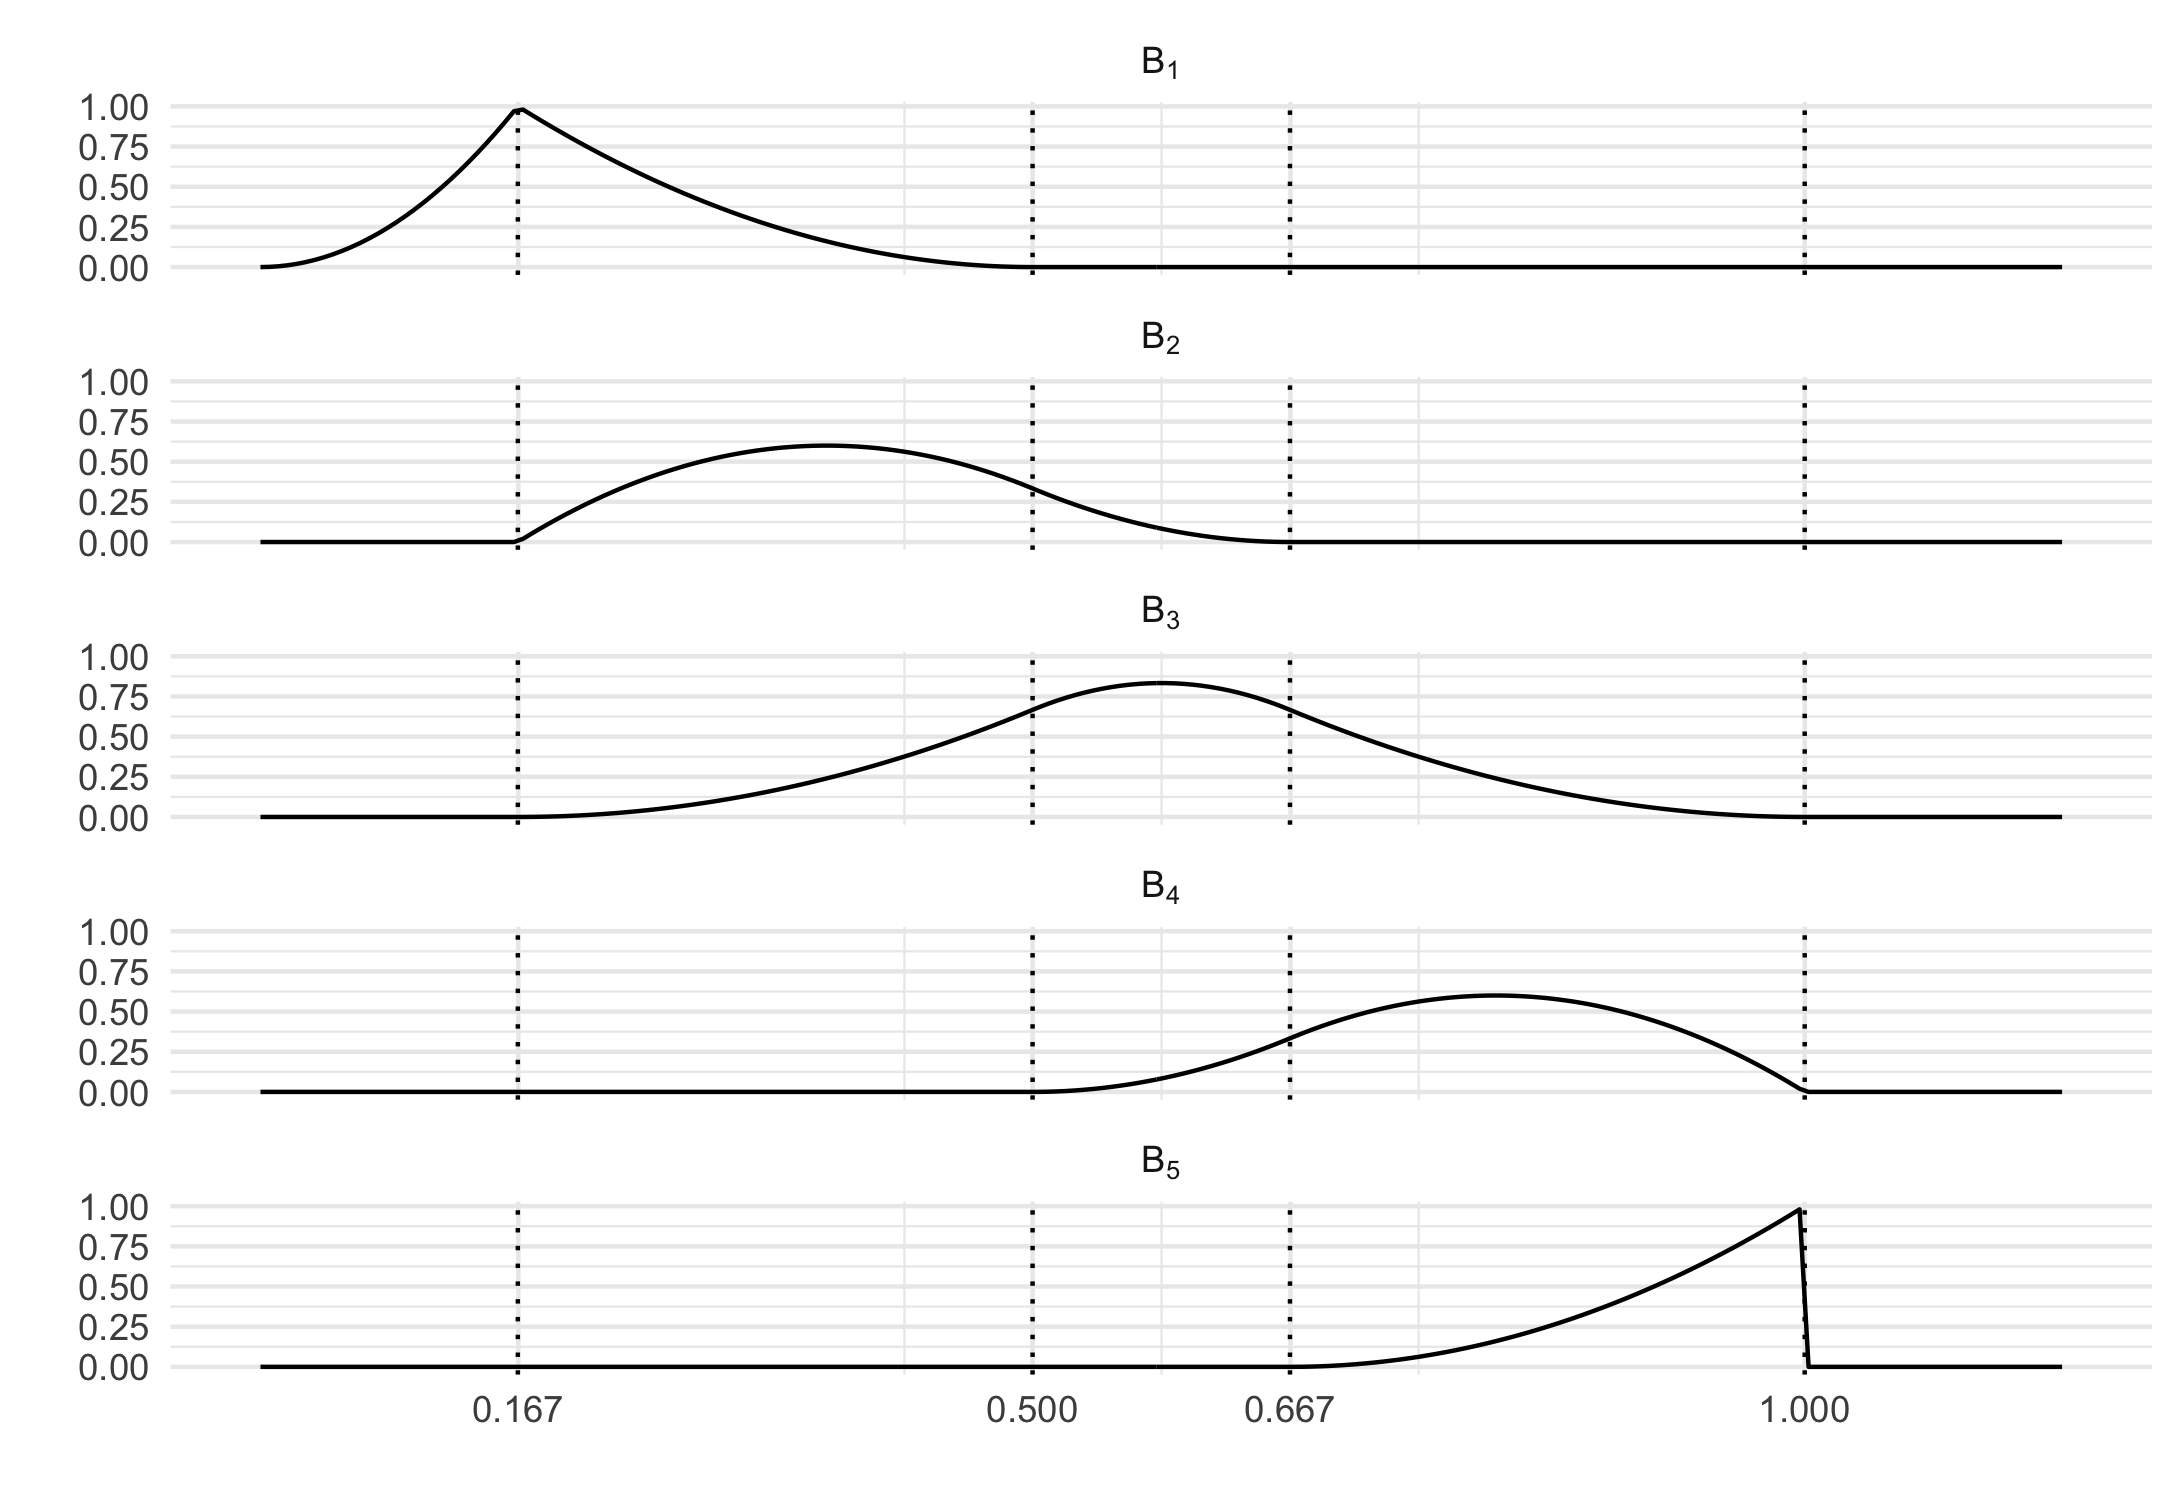
\includegraphics{deboor_parabolic_bsplines.png}
%  %\caption{Parabolic B-splines corresponding to knot sequence $\{0,1,1,3,4,6,6,6\}$, illustrating the connection between knot multiplicity and smoothness.}\label{fig:deboor_bspline_basis}
%\end{center}
%\end{figure}
%\end{example}


\begin{definition} \label{B_representation_definition}
The \emph{B-representation of } $f \in \PP_{k,\xi,\nu}$ consists of 
\begin{enumerate}
\item \label{eq:first_B_rep_piece} integers $k$ and $n$ specifying the order of $f$ as a pp function and the number of linear parameters, 
\[
n = kl - \sum_{i}\nu_i = \mbox{dim}\left(\PP_{k,\xi,\nu}\right),
\]
respectively. 
\item \label{eq:second_B_rep_piece}The knot vector $t = \left \{t_i \right\}$, $i=1,\dots, n+k$ with elements arranged in increasing order, constructed according to Theorem~\ref{curryschoenbergthm}, via $\xi$ and $\nu$.
\item \label{eq:third_B_rep_piece} The B-spline coefficients $\alpha=\left \{\alpha_i \right\}$, $i=1 ,\dots, n$ for the knot sequence, $t$.
\end{enumerate}
\end{definition}
\vspace{1pt}
Given \ref{eq:first_B_rep_piece}, \ref{eq:second_B_rep_piece}, and \ref{eq:third_B_rep_piece} in \ref{B_representation_definition}, the function value at $x\in \left[t_k, t_{n+1}\right]$ is given by 
\begin{equation*}
f\left(x\right) = \sum_{i=1}^n \alpha_i B_i\left(x\right),
\end{equation*}
and in particular, by \ref{eq:BS_property_1}, for $x\in \left[t_j, t_{j+1} \right]$,
\[
f\left(x\right) = \sum_{i=j}^{j+k-1} \alpha_i B_i\left(x\right).
\]





\section{Single-regressor varying coefficient models via B-spline basis expansions}

Hastie and Tibshirani were the first to introduce the varying coefficient model, which supplies a modeling approach which permits interpolation of regressors and response variables which varying according to an \emph{indexing variable} at values of this indexing variable where there is either missing data of only a single observation and slope estimation is not feasible. In the section that follows, we will discuss the approach to smoothing the coefficient vector (and \emph{not} the regressor, $x\left(t\right)$) first, for mechanical demonstration of parameterization and estimation of the coefficient function via B-spline basis expansion, at a predetermined set of values of an indexing variable, $t$ (knots), then following the approach of Eilers and Marx by assuming that the number and position of the knots are unknown and using penalized B-splines, or P-splines. 

Consider data of the form 
\[
\left(x_i, y_i, t_i\right), \qquad i=1,\dots,m
\]
where $y_i$ is the response, $x_i$ is the single (univariate) regressor variable, and $t_i$ is an indexing variable. We first consider a simple situation as an introductory warmup for demonstrating the mechanics of the varying coefficient model. Suppose we wish to fit a scatterplot smoother to the points $\left(t_i, y_i\right)$ using a B-spline basis expansion. Assume that we can model 

\begin{equation} \label{eq:varying_intercept_only_model}
y\left(t\right) = f\left(t\right) + \epsilon\left(t \right)
\end{equation}

where $\epsilon$ is a zero-mean error process.  Modeling the mean function as a $q^{th}$-order B-spline, we can rewrite \ref{eq:varying_intercept_only_model} as

\begin{equation} \label{eq:varying_intercept_only_model_bspline}
y\left(t\right) = \sum_{j=1}^{K} \alpha_j B_j\left(t\right) + \epsilon\left(t \right)
\end{equation}

Assume we use $K$ of basis functions in our expansion of $f$. Let $y= \left(y_1,\dots,y_m\right)^T$, and let $B$ denote the $m \times K$ design matrix with $i-j^{th}$ element given by the $j^{th}$ order-$q$ B-spline evaluated at the $i^{th}$ value of $t$: 

\[
b_{ij} = B_j\left(t_i\right),
\]
$i=1,\dots,m$, $j=1,\dots,K$. Then in matrix notation, we may write the mean vector

\[
\mu = E\left[y\right] = B\alpha
\]
\noindent
where $\alpha$ is the vector of $K$ unknown basis coefficients. We take $\hat{\alpha}$ to be the minimizer of 

\begin{align}
S &= \sum_{i=1}^m \left(y_i - \sum_{j=1}^{K} \alpha_j B_j\left(t_i\right) \right)^2 \nonumber\\
&=\vert y - B\alpha \vert^2 \label{eq:S_varying_intercept_model}
\end{align}


\[
B^TB\alpha = B^Ty
\]
which has explicit solution
\[
\hat{\alpha} = \left(B^T B\right)^{-1}B^Ty
\]

Given $\hat{\alpha}$, one may estimate the response at any new value of $t$, say $t^*$, by 
\[
\hat{y}\left(t^*\right) = \sum_{j=1}^{K} \hat{\alpha_j}B_j\left(t^*\right).
\]

\subsection{B-spline estimators for varying coefficient models with fixed knots}

To extend the varying intercept model \ref{eq:varying_intercept_only_model} to accommodate for controlling for another regressor, it is natural to consider the varying coefficient model; the single regressor varying-coefficient (VC) model extends the classical linear model by allowing the slope coefficient to vary smoothly in the dimension of the indexing variable, $t$.  The single-index varying coefficient model assumes that the mean response is of the form

\begin{equation} \label{eq:simplest_VC_model_mean}
E\left[ Y\left(t\right) \right] = \beta_0\left(t\right) + \beta_1\left(t\right)x\left(t\right)
\end{equation}

where $\beta_0\left(t\right)$ is the smooth varying intercept function and $\beta_1\left(t\right)$ is the smooth slope function of interest. This model generalizes the well known simple linear regression model 
\[
E\left[Y\left(t\right)\right] = \beta_0 + \beta_1 x\left(t\right)
\]
by trading the static regression coefficients for smooth coefficient functions which are assumed to varying across an indexing variable, $t$. This allows for the regressor variable to having modified effect, depending on the value of $t$. Using a set of predetermined knots along the $t$ axis, the VC model can be fit in a fashion similar to that required for fitting model \ref{eq:varying_intercept_only_model}, requiring only minor adjustments to the design matrix. In matrix notation as described in \ref{eq:S_varying_intercept_model}, the mean vector may be written

\begin{equation} \label{eq:VC_mean_matrix}
\mu = B\alpha_0 + diag\left\{x\left(t\right) \right\}B\alpha_1
\end{equation} 
\noindent
where $diag\left\{x\left(t\right) \right\}$ is the $m \times m$ diagonal matrix of regressor measurements which ensures that the varying coefficients are appropriately weighted according to the correct value of $x$ by aligning the regressor function with the corresponding slope value. Letting $U = diag\left\{x\left(t\right) \right\}B$, \ref{eq:VC_mean_matrix} becomes

\begin{align}
\mu &= \left[ B | U \right] \left(\alpha_0^T,\alpha_1^T\right)^T \\
&\equiv Q\alpha
\end{align} 

where $\alpha$ is the augmented vector of basis coefficients. Here, the same basis is used for smoothing both the varying intercept as well as the varying slope function; this is feasible because both components varying along the same indexing variable. One can relax this structure and allow each additive term to varying according to its own indexing variable. This, of course, requires a separate B-spline basis for each component. Again using least squares techniques as with the varying intercept-only model, we take $\hat{\alpha}$ to minimize

\begin{equation} \label{eq:S_varying_intercept_slope_model}
S = \vert y-Q\alpha \vert ^2
\end{equation}
which has explicit solution

\[
\hat{\alpha} =\left(Q^T Q\right)^{-1} Q^Ty.
\]

It is of interest to notice that $Q$ is simply a row scaling of the original B-spline design matrix, $B$; thus, accommodating a varying slope function equates to the simple basis function regression setting with a modified basis, $UB$. Using the modified basis functions as covariates, estimation of model the varying coefficient model equates to a multiple regression problem. Each of the estimated smooth components are given by 
\[
\hat{\beta}_k\left(t \right)= B\hat{\alpha}_k, \qquad k=0,1
\]
\noindent
and the estimate of the smooth mean function is obtained via 
\begin{align*}
\hat{\mu} &= Q\hat{\alpha}\\
&= Hy
\end{align*}
where $H = Q\left(Q^T Q\right)^{-1} Q^T$ is the ``hat'' matrix. This will be discussed in further detail in later sections on smoothing parameter selection and model tuning.





%%==============================================================================================================================================
%%==============================================================================================================================================
%%==============================================================================================================================================





\section{P-spline estimators for regularized estimation of fitted curves}

The mechanics in the previous section rely on apriori knowledge of the number and locations of the knots $\left\{t_j\right\}$, $j=1,\dots,K$. In practice this information is readily available, but has a considerable impact on the behaviour of the estimated coefficient functions, as the smoothness of a fitted curve can be controlled by the number of B-splines used in the basis expansion used to approximate the curve. Fewer knots (thus, fewer basis functions) lead to smoother fits. This choice presents a model selection problem, as too many knots lead to overfitting while too few knots lead to underfitting. Optimal knot placement has been closely examined, with some authors proposing automatic methods for optimizing the number and the positions of the knots (Friedman and Silverman, 1989; Kooperberg and Stone, 1991,1992). This is a difficult numerical problem requiring nonlinear optimization, and is still an open problem today. However, limiting the number of B-splines is not the only approach to controlling the complexity of the fitted function. 

As in chapter {\needsparaphrased{smoothing spline chapter}}, we can append a penalty on the coefficients of the basis functions to the goodness of fit measure, and by optimizing this augmented objective function, we can achieve as much smoothness in the fitted function as desired. cite{o1986statistical} was the first to propose using a rich B-spline basis and applying a discrete penalty to the spline coefficients. 

 He proposed a penalty on the second derivative to restrict the flexibility of the fitted curve, similar to the penalty pioneered for smoothing splines by Reinsch (1967). This penalty has become the standard in much of the spline literature; see Eubank (1988), Wahba (1990) and Green and Silverman (1994). This measure of roughness of a curve is given by 
 
 \[
 J = \int_l^u \left[ f^{\prime \prime}\left(x\right)\right]^2\;dx
 \]
 \noindent
 where $l$ and $u$ are the bounds on the domain of $x$. Using the properties of B-splines, if $f\left(x\right) = \sum_{j} \beta_j B_j\left(x\right)$, one can derive a banded matrix $P$ such that 
 \[
 J = \beta^\prime P \beta
 \] 
 \noindent
 where $\beta = \left(\beta_1,\dots, \beta_n\right)$, and the $i$-$j^{th}$ element of $P$ is given by
 \[
 p_{ij} = \int_l^u B_i^{\prime \prime} \left( x \right)B_j^{\prime \prime} \left( x \right)\;dx.
 \]
 \noindent
 He then proposed minimizing
 \begin{eqnarray*}
 Q\left(\beta, \lambda \right) &=& \sum_{i=1}^m \left(y_i - \sum_{j} \beta_j B_j\left(x_i \right)\right)^2 + \lambda \int_l^u \left[ f^{\prime \prime}\left(x\right)\right]^2\;dx\\
 &=& \vert y - B\beta \vert  \vert^2 + \lambda\beta^\prime P \beta
 \end{eqnarray*}

The computation of $P$ is nontrivial and becomes very tedious when the third and fourth derivative are used as the roughness measure. cite{wand2008semiparametric} extend O'Sullivan's work to higher order derivatives for general degree B-splines and derive an exact matrix algebraic expression for the penalty matrices. In the cubic case, the expression is a result of the application of Simpson's Rule applied to the inter-knot differences since each $B_i^{\prime \prime} B_j^{\prime \prime}$ is a piecewise quadratic function. The penalty may be written
 \[
 P = \left(B^{\prime \prime}\right)^\prime \textup{diag}\left(\omega \right) B^{\prime \prime}, 
 \]
 \noindent
 where $B^{\prime \prime}$ is the $3\left( n + 7 \right) \times \left( n + 4 \right)$ matrix with $i$-$j^{th}$ entry given by $B_j^{\prime \prime} \left(x_i^*\right)$, $x^*_i$ is the $i^{th}$ element of 
 
\[
\left( \phi_1,\frac{\phi_1+\phi_2}{2},\phi_2,\phi_2,\frac{\phi_2+\phi_3}{2},\phi_3,\dots,\phi_{n+7},\frac{\phi_{n+7}+\phi_{n+8}}{2},\phi_{n+8} \right),
\]
 \noindent
 and $\omega$ is the $3\left(n+7\right) \times 1$ vector given by
 
\begin{align*}
\omega &= \left( \frac{1}{6}\left(\Delta \phi \right)_1,\frac{4}{6}\left(\Delta \phi \right)_1, \frac{1}{6}\left(\Delta \phi \right)_1,\frac{1}{6}\left(\Delta \phi \right)_2, \frac{4}{6}\left(\Delta \phi \right)_2,  \right. \\
&\qquad   \left. {} \frac{1}{6}\left(\Delta \phi \right)_2 , \dots , \frac{1}{6}\left(\Delta \phi \right)_{n+7}, \frac{4}{6}\left(\Delta \phi \right)_{n+7}, \frac{1}{6}\left(\Delta \phi \right)_{n+7}  \right) \\
\end{align*}
\noindent
 where $\left(\Delta \phi \right)_j = \phi_{j+1}-\phi_j$. They generalize this to the case of any order penalty and present a table of formulas for constructing any arbitrary penalty matrix, $P$.
 
 %%==============================================================================================================================================
 
 \subsection{Difference penalties}
 
Imposing difference penalties on B-spline basis expansions generalizes and simplifies the approach outlined in the previous section in a way that permits application in any context where regression on B-splines is useful. Penalized B-splines, or \emph{P-splines}, are an alternative an approach to nonparametric smoothing which circumvent any complexity associated with constructing such penalty matrices by ommitting derivatives and integrals altogether. Instead, smoothness is imposed via a discrete penalty matrix based on finite difference formulas which is simple to compute. This approach achieves smoothness in fitted functions in two ways:

\begin{enumerate}
\item To avoid the difficulty of choosing the optimal set of knots, use a B-spline basis with a large number of equally spaced knots, purposefully overfitting the smooth coefficient vectors. 
\item Augment the goodness of fit measure with a difference penalty to prevent overfitting and accomodate a potentially ill-conditioned fitting procedure.
\end{enumerate}  
 
Using the properties of B-splines derived in {\needsparaphrased{B-spline section}}, it is relatively straightforward to show that the simplified penalty is nearly equivalent to the derivative-based penalty and that for second order differences, P-splines are very similar to O'Sullivan's approach. In some applications, it can be useful to use differences of a smaller or higher order in the penalty, and the P-spline framework makes the use of a penalty of any arbitrary order nearly seamless. 
 
Consider the varying intercept-only model defined in \ref{eq:varying_intercept_only_model} for the regression of $M$ data points $\left(t_i,y_i\right)$ on a set of $K$ B-splines, $\left\{B_j\right\}$.  By letting the number of knots, $K$, be relatively large, we allow more variation in fitted curve than the data reasonably justify. To make the result less flexible and avoid overfitting, O'Sullivan imposed a penalty on the second derivative of the fitted curve and appended this to the residual sum of squares, giving way to the objective function

\begin{equation} \label{eq:univariate_bspline_ridge_penalty}
\sum_{i=1}^m \left \{ y_i - \sum_{j=1}^K \beta_j B_j\left(t_i\right) \right \}^2 + \lambda \int_{t_{min}}^{t_{max}} \left\{  \sum_{j=1}^K \beta_j B^{\prime \prime}_j\left(t\right) \right\}^2 \; dt.
\end{equation}

The integral of the square of the second derivative of a fitted function has become common as a smoothness penalty since the seminal work on smoothing splines by Reinsch (1967), though it is useful to note that there is nothing particularly special about the second derivative. One could easily specify higher or lower order derivatives in smoothness penalties. In the context of smoothing splines, the first derivative leads to simple equations and a piecewise linear fit, while higher derivatives lead to systems of equations with a high bandwidth and a very smooth fit. 


Proposed for smoothing curves by cite{whittaker1922new}, difference penalties have been utilized for nearly a century, with more recent applications  outlined in  cite{eilers1991penalized}, cite{eilers1991nonparametric}, and cite{eilers1995indirect}. The finite difference penalty is easily introduced into regression equations, making it feasible to evaluate the impact of different orders of the differences on the fitted model. In some applications, it is useful to work with third and fourth order differences, since for high values of $\lambda$, the fitted curve approaches a parametric polynomial model. Detailed discussion on the effect of the smoothing parameter on fitted functions will follow. Let $D_d$ denote the matrix difference operator; that is, $D_d\beta = \Delta^d \beta$, where

 \begin{eqnarray*}
 \Delta \alpha_j &=& \alpha_j - \alpha_{j-1},\\
 \Delta^2 \alpha_j &=& \Delta\left(\Delta \alpha_j\right) = \alpha_j - 2\alpha_{j-1} + \alpha_{j-2},\\ 
 \end{eqnarray*}
\noindent 
and in general,
\begin{equation*}
\Delta^d \alpha_j = \Delta\left(\Delta^{d-1} \alpha_j \right)
\end{equation*}
The $\left(K - d\right) \times K$ differencing matrix $D_d$ is sparse for reasonably small values of $d$; for example, $D_1$ and $D_2$ for small dimensions are given by 
\[
D_1 = \begin{bmatrix} -1&1&0&0\\ 0&-1&1&0\\ 0&0&-1&1 \end{bmatrix}; \qquad D_2 = \begin{bmatrix} 1&-2&1&0 \\ 0&-&-2&1\end{bmatrix}
\]

cite{eilers1996flexible} propose to base the penalty on (higher-order) finite differences of the coefficients of adjacent B-splines:

 \[
 \lambda\vert D_d\alpha\vert^2 = \lambda \alpha^\prime D^\prime_d D_d \alpha = \lambda \alpha^\prime P\alpha,
 \] 



Replacing O'Sullivan's penalty with the difference penalty, we can control the smoothness of the fitted mean function $\mu = \beta_0\left( t \right) = B\alpha$ by minimizing
\begin{equation*} 
S_\lambda = \vert y- B \alpha \vert^2 + \lambda\vert D_d\alpha \vert^2
\end{equation*}

This approach reduces the dimensionality of the problem to the number of B-splines, $K$ instead of the number of observations, $M$ , as with smoothing splines. The tuning parameter $\lambda$ permits continuous control over smoothness of the fit. We will demonstrate that the difference penalty is a good discrete approximation to the integrated square of the $k^{th}$ derivative, and with this penalty, moments of the data are conserved and polynomial regression models occur as limits for large values of $\lambda$. We will explore the connection between a penalty on second-order differences of the B-spline coefficients and O'Sullivan's choice of a penalty on the second derivative of the fitted function. However, the difference penalty can be handled mechanically for any order of the differences.
cite{o1986statistical} used third-degree B-splines and the following penalty:

\begin{equation} \label{eq:osullivan_univariate_bspline_penalty}
h^2 P = \lambda \int_{t_{min}}^{t_{max}} \left\{ \sum_{j}  \alpha_j B_{j,3}^{\prime \prime} \left(t\right) \right\}^2\; dt
\end{equation}
\noindent
From the derivative properties of B-splines, it follows that
\begin{equation} \label{osullivan_univariate_bspline_penalty_via_deriv}
h^2 P = \lambda \int_{t_{min}}^{t_{max}}  \sum_{j} \sum_{k} \Delta^2 \alpha_j \Delta^2 \alpha_k B_{j,1}\left(t\right)B_{k,1}\left(t\right) dt 
\end{equation}
\noindent
Most of the cross products of $B_{j,1}(t)$ and $B_{k,1}(t)$ vanish since B-splines of degree 1 only overlap when $j$ is $k-1$, $k$, or $k+1$. Thus, we have that
\begin{align}
h^2 P = {} & \lambda \int_{t_{min}}^{t_{max}} \bigg[ \left\{ \sum_{j}  \Delta^2 \alpha_j  B_j\left(t,1\right)  \right\}^2  + 2 \sum_{j}\Delta^2 \alpha_j\Delta^2 \alpha_{j-1}B_j\left(t,1\right)B_{j-1}\left(t,1\right) \bigg] dt \nonumber \\ 
= {} & \lambda \bigg[ \sum_j \left( \Delta^2\alpha_j \right)^2 \int_{t_{min}}^{t_{max}} B_j^2\left(t,1\right)\;dt + 2 \sum_j \Delta^2 \alpha_j\Delta^2 \alpha_{j-1} \bigg]
\end{align}
\noindent
or
\begin{align}
h^2 P = \lambda \sum_j \left( \Delta^2\alpha_j \right)^2 \int_{t_{min}}^{t_{max}} B_{j,1}^2\left(t\right) dt {} & +  2\lambda \sum_j \Delta^2 \alpha_j \Delta^2 \alpha_{j-1}  \nonumber \\ 
{} &+\int_{t_{min}}^{t_{max}} B_{j,1}\left(t\right)B_{j-1,1}\left(t\right) dt
\end{align}
\noindent
which can be written as
\begin{equation} \label{eq:osullivan_penalty_decomp}
h^2 P = \lambda\left\{c_1 \sum_j\left( \Delta^2 \alpha_j\right)^2 + c_2 \sum_j\Delta^2 \alpha_j\Delta^2 \alpha_{j-1} \right\}
\end{equation}
\noindent
where, for given equidistant knots, $c_1$ and $c_2$ are constants given by
\begin{equation}
\begin{split}
c_1 & =   \int_{t_{min}}^{t_{max}} B_{j,1}^2\left(t\right) dt\\
c_2 & = \int_{t_{min}}^{t_{max}} B_{j,1}\left(t\right)B_{j-1,1}\left(t\right) dt
\end{split}
\end{equation}

O'Sullivan's ridge-like B-spline penalty in Equation~\ref{eq:osullivan_univariate_bspline_penalty} can be written as a linear combination of a difference penalty (\ref{eq:univariate_pspline_diff_penalty}) and the sum of the cross products of neighboring second differences. The second term in Equation~\ref{eq:osullivan_penalty_decomp} leads to a complex objective function when minimizing the penalized likelihood, where seven adjacent spline coefficients occur, as opposed to five if only the first term in Equation~\ref{eq:osullivan_penalty_decomp} is used in the penalty. The additional complexity is due to overlapping B-splines, which quickly increases when using higher order differences and higher order B-splines. The use of a difference penalty allows us to sidestep the difficulty of constructing a procedure for incorporating the penalty in the likelihood equations. 

Define $\hat{\alpha} = \left(\hat{\alpha}_1, \hat{\alpha}_2, \dots, \hat{\alpha}_K \right)$ to be the minimizer of $S_\lambda$:

\begin{equation*}  
S_\lambda = \sum_{i=1}^m \left\{ y_i - \sum_{j=1}^K \alpha_j B_j\left(t_i\right) \right\}^2 + \lambda \sum_{j=d+1}^K \left( \Delta^d\alpha_j \right)^2
\end{equation*}
\noindent
In vector notation, this may be written

\begin{align}
\begin{split}
S_\lambda &= \vert y- B\alpha  \vert^2  + \lambda \vert D_d \alpha\vert^2 \\
&=  \left( y- B\alpha  \right)^T \left( y-B \alpha\right) + \lambda \alpha^T P \alpha
\end{split} \label{eq:S_pen_varying_intercept_model}
\end{align}
\noindent
where 
\[
P = D_d^T D_d
\]
\noindent
and the elements of $B$ are given by $b_{ij} = B_j\left(t_i\right)$, as defined in \ref{eq:S_varying_intercept_model}. Taking derivatives on both sides of \ref{eq:S_pen_varying_intercept_model} with respect to $\alpha$ gives

\begin{align}
\frac{\partial}{\partial \alpha}S_\lambda ={} & \frac{\partial}{\partial \alpha}\left(\alpha^TB^TB \alpha -2y^T B^T\alpha+\lambda \alpha^T D_k^T D_k \alpha  \right) \nonumber \\
= {} & 2B^TB \alpha - 2B^T y + 2\lambda D_d^TD_d\alpha \nonumber\\
= {} & \left(B^T B +  \lambda D_d^TD_d\right)\alpha - B^T y \label{eq:dSlambda_dAlpha}
\end{align} 
\noindent

and setting equal to zero yields normal equations:
\begin{equation}\label{eq:S_lambda_normal_eq}
B^T y = \left(B^T B +  \lambda D_d^TD_k\right)\alpha,
\end{equation}
which has explicit solution
\[
\hat{\alpha} = \left(B^T B +  \lambda D_d^TD_d\right)^{-1}B^T y
\]
\noindent
The effective hat matrix is now
\[
H_\lambda - B\left(B^T B +  \lambda D_k^TD_k\right)^{-1}B^T 
\]

When $\lambda = 0$, we have the standard normal equations of linear regression with a B-spline basis, and with $k = 0$ \ref{eq:S_lambda_normal_eq} corresponds to the normal equations under the ridge regression penalty. When $\lambda > 0$, the penalty only influences the main diagonal and $k$ sub-diagonals of the system of equations. The compact support and limited overlap of the B-spline basis functions gives this system a banded structure, though exploiting this structure is of little utility since the number of equations is equal to the number of splines, which is generally moderate by design. 



\subsubsection{P-splines for single-index VC models}

The derivations in the previous section requiring little adjustment for accommodating a regressor and its corresponding varying slope function, as defined in Equation~\ref{eq:simplest_VC_model_mean} with $\mu\left(t\right) =  Q\alpha$, where 
\[
Q = \left[B | diag\left\{x\left(t\right) \right\}B \right]
\]
but now $B$ holds a rich B-spline basis with equally-spaced knots. If one wishes to allow for differing degrees of smoothing for each of the varying intercept term and the slope function, the P-spline objective function \ref{eq:S_pen_varying_intercept_model} must be further modified to accommodate multiple tuning parameters, $\lambda_i$, $i=0,1$. The objective function then becomes
\begin{align} 
\begin{split}
S^*_\lambda &= \vert y- Q\alpha  \vert^2  + \lambda_0 \vert D_{d_0} \alpha_0 \vert^2 + \lambda_1 \vert D_{d_1} \alpha_1 \vert^2\\
	&= \vert y- Q\alpha  \vert^2  + \vert \alpha^T P \alpha \vert^2
\end{split} \label{eq:S_pen_star}
\end{align}

where the penalty has form $P = \mbox{block diag}\left(\lambda_0 D_{d_0}^TD_{d_0}, \lambda_1 D_{d_1}^TD_{d_1} \right)$. The minimizer of \ref{eq:S_pen_star} is given by
\[
\hat{\alpha} = \left(Q^T Q +  P\right)^{-1}Q^T y.
\]

The block diagonal structure of the penalty separates the penalization of each individual smooth component. The estimated mean function is then given by 
\[
\hat{\mu} = Q \hat{\alpha} = H y
\] 
where
\begin{equation} \label{eq:simplest_VC_model_hat_matrix}
H = Q\left(Q^T Q +  P\right)^{-1}Q^T.
\end{equation}

{\needsparaphrased{[Figure~\ref{fig:PS_VCM_section_figure_1} Need to explain figure 3 here. ]} }

\begin{figure}[H]
   \graphicspath{{img/}}
   \centering
  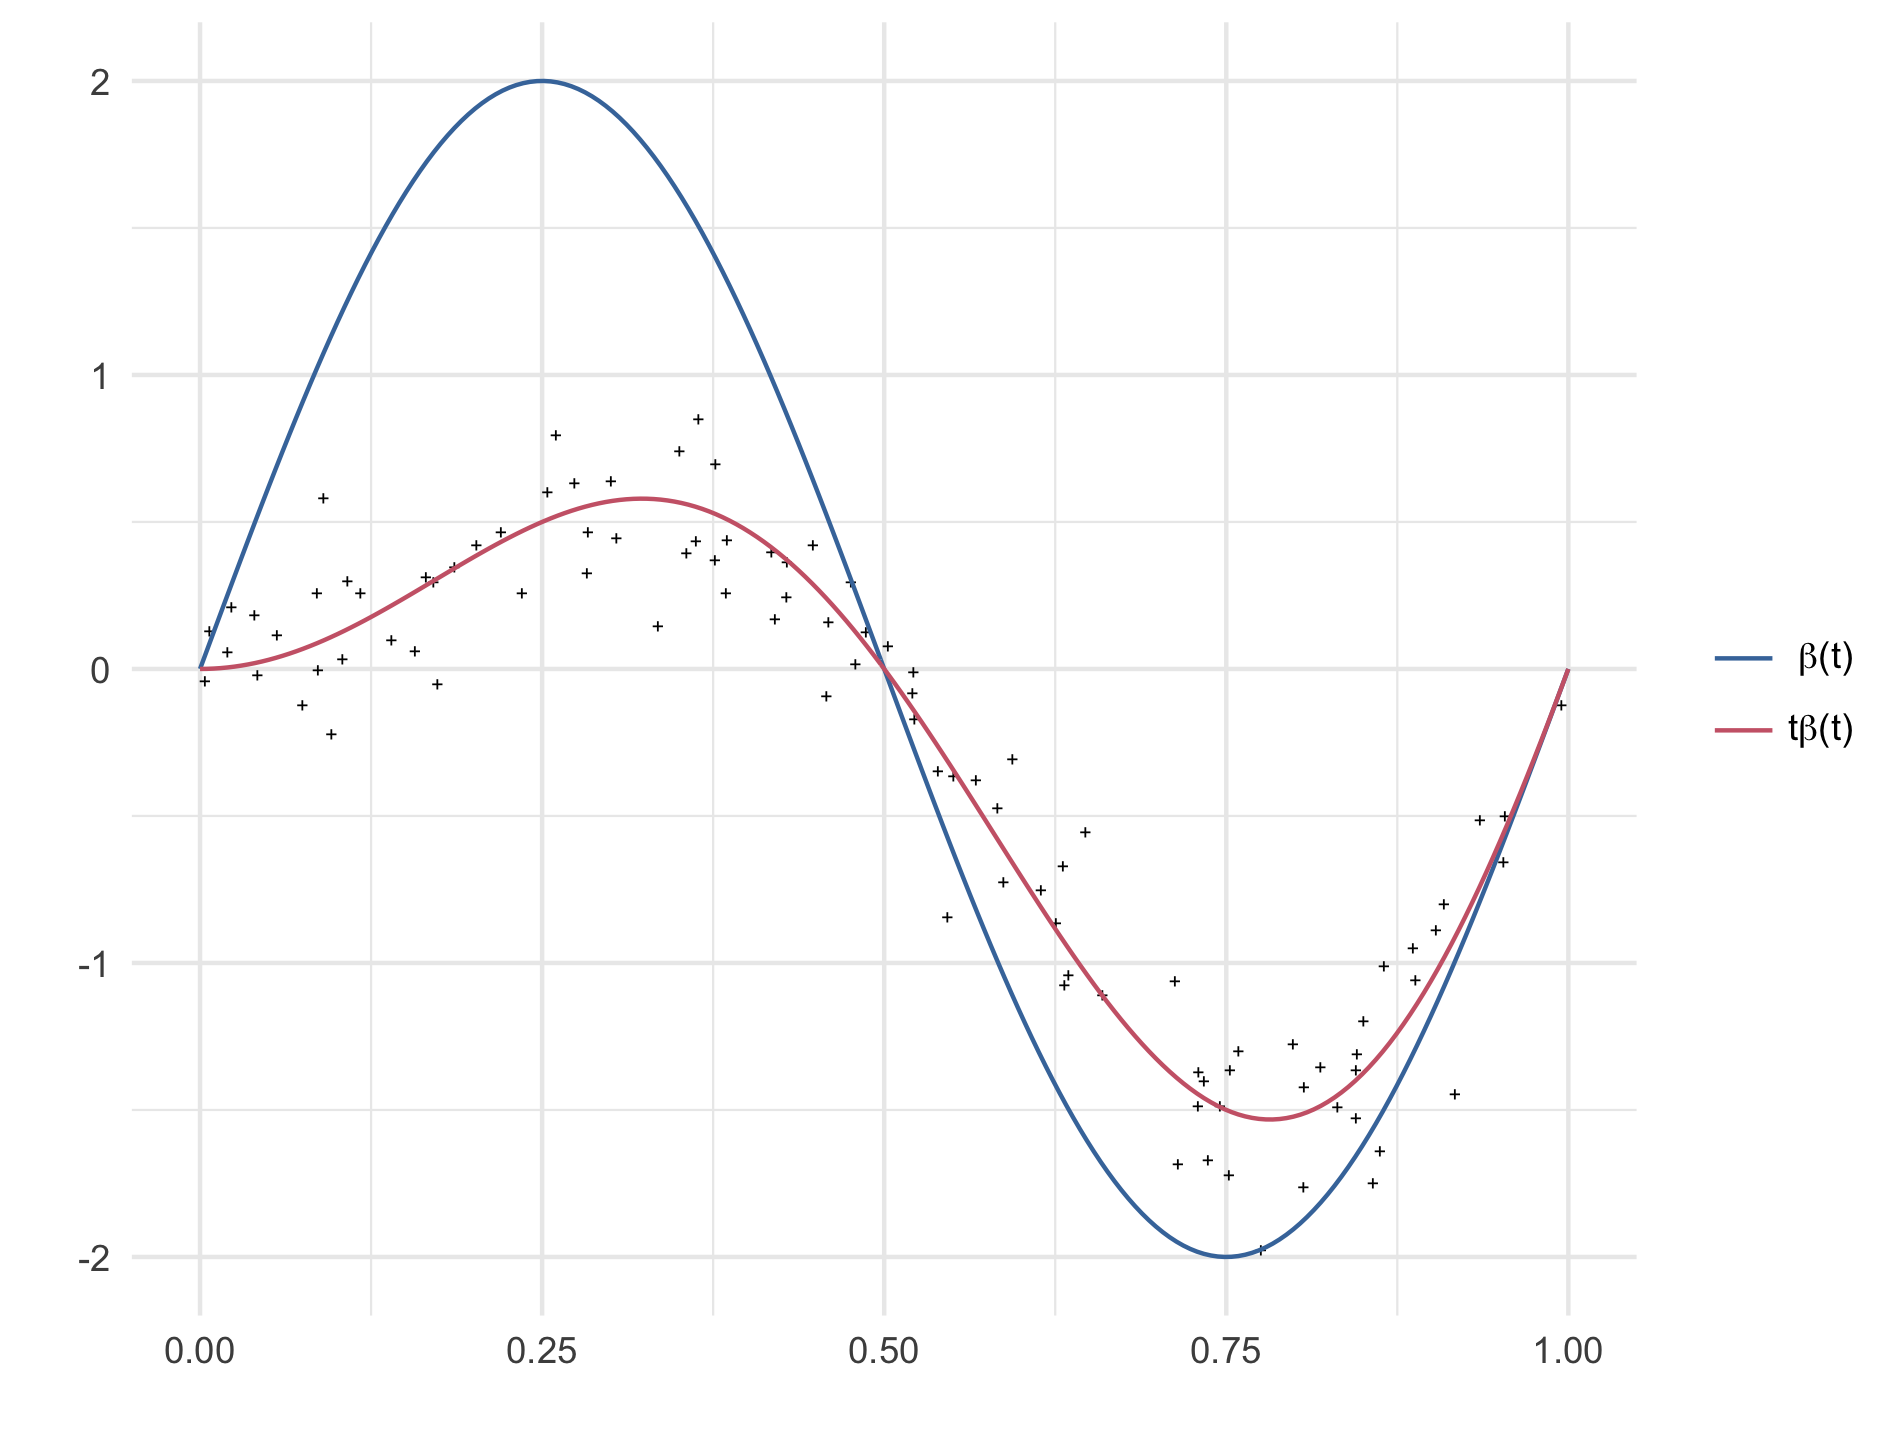
\includegraphics[scale=0.25]{PS_VCM_section_figure_1.png}
\caption{\textit{100 simulated data points where} $y\left(t\right) = t \beta\left( t \right) + 0.2\epsilon\left(t\right)$ \textit{where} $\epsilon$ \textit{is a white noise process with unit variance, and} $\beta\left(t\right) = 2\sin\left(2\pi t\right)$.}
\label{fig:PS_VCM_section_figure_1}
\end{figure}

\begin{figure}[H]
 \begin{subfigure}{.48\textwidth}
  \centering
   \graphicspath{{img/}}
 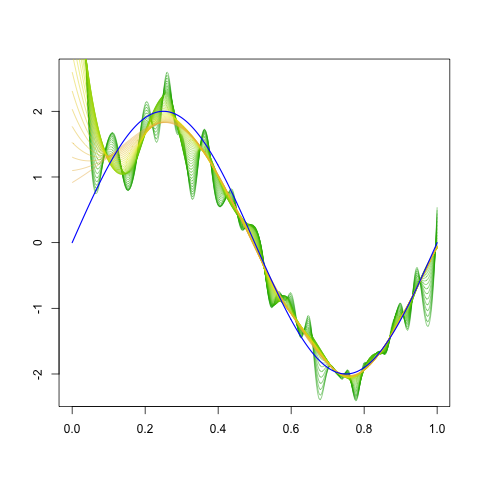
\includegraphics[scale=0.5]{PS_VCM_section_figure_2.png}
 \caption{$\hat{\beta}\left(t\right)$}
 \end{subfigure}
 \begin{subfigure}{.48\textwidth}
  \centering
   \graphicspath{{img/}}
  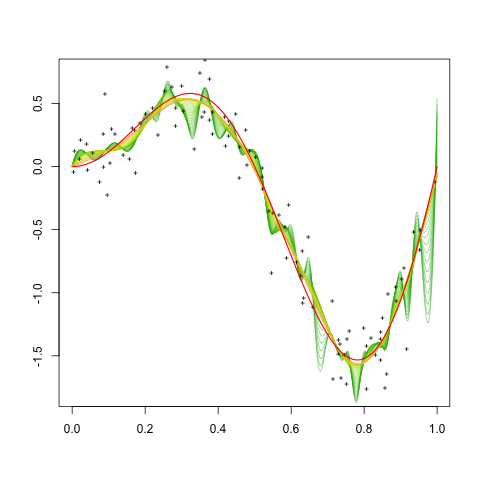
\includegraphics[scale=0.5]{PS_VCM_section_figure_3.png}
 \caption{$\hat{\mu}\left(t\right) = t \hat{\beta}\left(t\right)$}
\label{fig:PS_VCM_section_figure_2}
 \end{subfigure}
 \caption{\textit{Estimated coefficient function} $\hat{\beta}\left(t\right)$ \textit{and mean curve} $\hat{\mu}\left(t\right) = t \sin(2 \pi t)$ \textit{using a 80 B-splines basis functions of order 5 and a difference penalty of order} $k=3$.}
\end{figure}

The properties discussed in Section~\ref{BS_properties_continued} allude to how controlling the coefficients of a spline $f \in \mathscr{S}_{k,t}$ influences the shape of the overall function. Specifically, the form of the $j^{th}$ derivative provides an avenue of understanding how the differenced B-spline coefficient sequence is related to the volatility of the function on a given interval of its domain. The following figure visually explore the impact of the squared distance on adjacent basis coefficients on the function; a useful way of examining at P-splines is to consider the coefficients as the skeleton of the function, then draping the B-splines over them to put the flesh over the bones. A smoother sequence of coefficients leads to a smoother curve, which is clearly illustrated in Figure~\ref{fig:second_ord_PS_pen_SML_lambda}. As long as the coefficient sequence is smooth, the number of basis functions (and coefficients) is unimportant. The penalty ensures the smoothness of the skeleton.

\begin{figure}[H]
\begin{subfigure}{.5\textwidth}
  \centering
   \graphicspath{{img/}}
  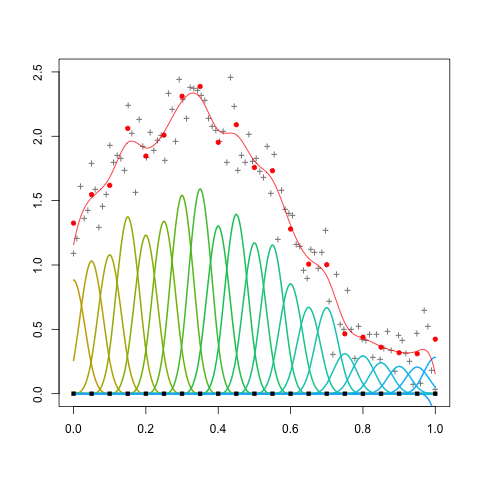
\includegraphics[scale=0.5]{pspline_pord2_xsmall_lambda.png}
  \label{fig:pspline_small_lambda}
\end{subfigure}
\begin{subfigure}{.5\textwidth}
  \centering
   \graphicspath{{img/}}
  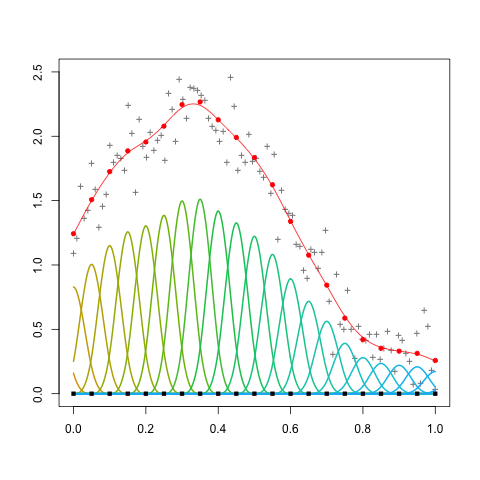
\includegraphics[scale=0.5]{pspline_pord2_small_lambda.png}
  \label{fig:pspline_small_lambda}
\end{subfigure}
\begin{subfigure}{.5\textwidth}
  \centering
   \graphicspath{{img/}}
  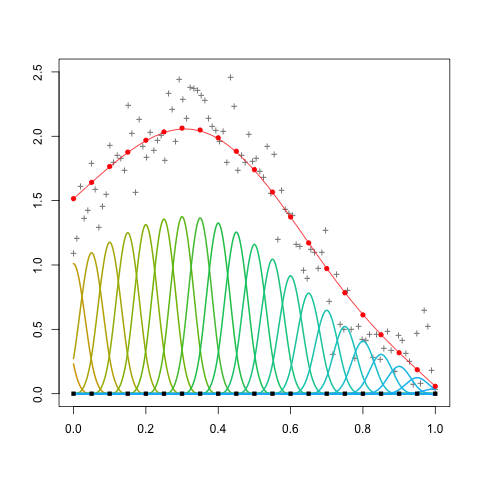
\includegraphics[scale=0.5]{pspline_pord2_medium_lambda.png}
  \label{fig:pspline_small_lambda}
\end{subfigure}
\begin{subfigure}{.5\textwidth}
  \centering
   \graphicspath{{img/}}
  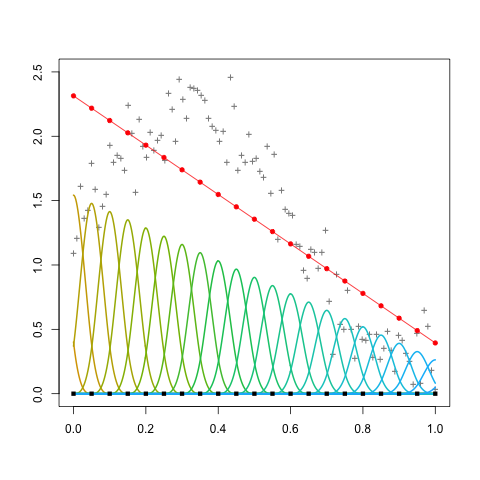
\includegraphics[scale=0.5]{pspline_pord2_large_lambda.png}
  \label{fig:pspline_small_lambda}
\end{subfigure}
\caption{\textit{Illustration of the impact of the second order difference penalty. The number of B-splines used is the same in each plot, with the value of the penalty parameter increasing from left to right and top to bottom across each plot. The fitted curve in the upper left plot is the most ``wiggly'' of any of the fits, as the penalty plays the weakest roll in the fitted coefficients there. The red circles are the values of each of the B-spline coefficients; as the penalty increases, they form as smoother sequence as we move across the four plots, which results in a smoother fitted function. As the penalty parameter approaches infinity, the fit approaches a linear function as shown in the bottom right plot.}}
\label{fig:second_ord_PS_pen_SML_lambda}
\end{figure}

The number of B-splines can be much larger than the number of observations because penalty ensures that the fitting procedure well-conditioned. One could literally use a thousand splines to fit ten observations without problems. Figure~\ref{fig:overcomplete_basis_pspline} illustrates this utility of the penalty for simulated data. There are $m=10$ observations and $40 + 3$ cubic B-splines. This property of P-splines cannot be overly appreciated, as it allows us to completely circumvent the nontrivial task of the optimal selection of knot placement. But one simply cannot have too many B-splines. Unless computational constraints are of concern, which is possible with large models, it is prudent to use even more. Figure~\ref{fig:PS_penalty_section_figure_3} shows how the fitted function changes as the tuning parameter $\lambda$ is varied in the presence of sparsely sampled data. 

\begin{figure}[H]   \label{fig:overcomplete_basis_pspline}
  \centering
   \graphicspath{{img/}}
  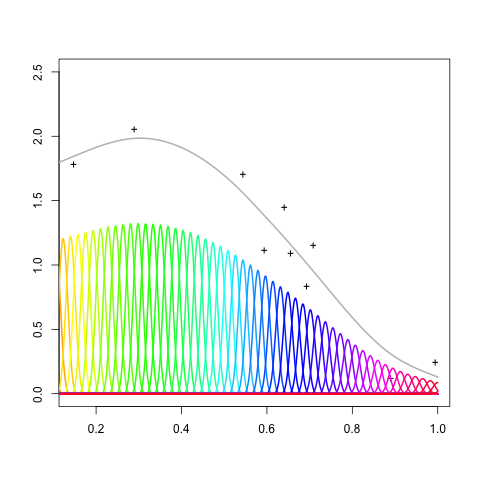
\includegraphics[scale=0.75]{pspline_10obs_60_basis_functions.png}
  \caption{P-spline smoothing of 10 observations using 60 B-spline basis functions.}
\end{figure}

\begin{figure}[H] \label{fig:PS_penalty_section_figure_3}
\centering
 \graphicspath{{img/}}
  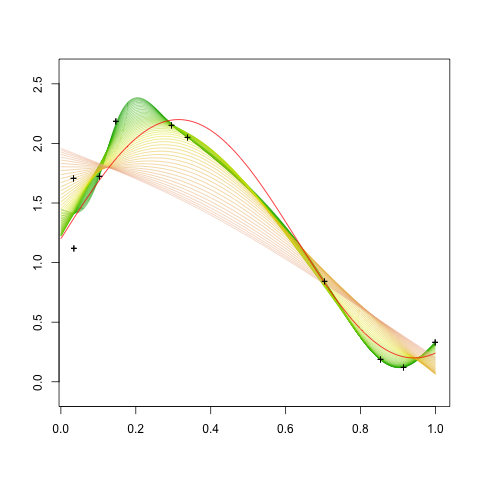
\includegraphics[width=4in, height=4in]{PS_penalty_section_figure_3.png}

  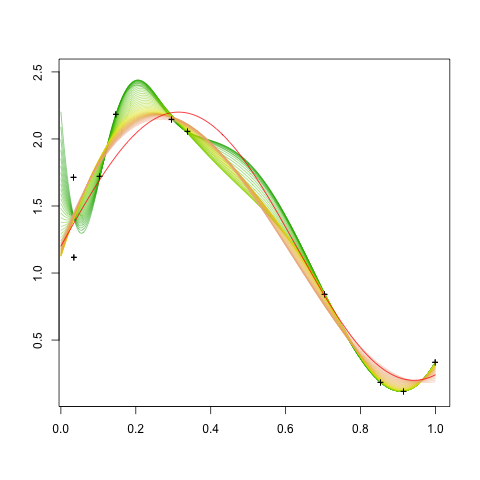
\includegraphics[width=4in, height=4in]{PS_penalty_section_figure_4.png}
 \caption{Fitted mean curves using a second (top) and third (bottom) order difference penalty for simulated data, sparsely sampled along the indexing variable: $y\left(t\right) = 1.2 + \sin\left(5t\right) + 0.2\epsilon_t$, where $\epsilon_t \stackrel{i.i.d.}{\sim}\textup{N}\left(0,1\right)$. A total of 10 data points were fit using a basis of 60 B-splines of degree $k=3$.}
\end{figure}

%%====================================================================================

\subsection{Properties of P-splines}

P-splines enjoy many advantageous properties, many due in part to the inherited properties of the B-spline basis functions on which a generous portion of their foundation is constructed. 

\begin{enumerate} \label{eq:PS_properties}
\item \begin{description}\item[Boundary effects]
 P-splines show no boundary effects, as many types of kernel smoothers do. By this, we mean the spreading of a fitted curve or density outside of the (physical) domain of the data, generally accompanied by bending toward zero.
\end{description}
\item \begin{description}\item[P-splines fit polynomial data exactly.] 
P-splines can fit polynomial data exactly. Given data $\left(t_i,y_i\right)$, if the $y_i$ are a polynomial in $t$ of degree $k$, then B-splines of degree $k$ or higher will fit the data exactly. 
\begin{proof}
This statement is equivalent to the claim that given $\xi = \left\{ \xi_i \right\}$, $i=1,\dots,l+1$, and $g$ such that $y\left(t\right) = g\left(t\right)$, we can find an $f \in \PP_{k,\xi} \bigcap \mathscr{C}^{\left(k-2\right)}$ which agrees with $g$ at the points $\tau_1 < \dots < \tau_n$  with $\tau_i \in \left[\xi_1,\xi_{l+1}\right]$ for all $i$, where
\[
n=k+l-1
\]
The solution, $f$ is constructed as follows: generate the knot sequence $t = \left\{t_i\right\}$ as per the recipe in Theorem~\ref{curryschoenbergthm}:
\begin{align*}
t_1 &= t_2 = \dots = t_k = \xi_1 & \\
t_{k+i} &= \xi_{i+1}, & i=1,\dots,l-1\\
t_{n+1} &= t_{n+2} = \dots = t_{n+k} = \xi_{l+1} & 
\end{align*}

Let $\left\{ B_{ik} \right\}$, $i=1,\dots,n$ be the corresponding sequence of B-splines of order $k$, which are a basis for $\PP_{k,\xi} \bigcap \mathscr{C}^{\left(k-2\right)}$ by Theorem~\ref{curryschoenbergthm}. Here, $\PP_{k,\xi} \bigcap \mathscr{C}^{\left(k-2\right)}$ denotes the space of pp functions with breakpoints $\xi$ having two continuous (global) derivatives. Then, cite{schoenberg1953polya} have shown that there exists exactly one $f \in \PP_{k,\xi} \bigcap \mathscr{C}^{\left(k-2\right)}$ agreeing with $g$ at $\tau_1,\dots, \tau_n$ if and only if 
\[
B_{ik}\left(\tau_i\right) \ne 0, \qquad \qquad i=1,\dots,n.
\]
This $f$ has a unique expansion of the form
\[
f = \sum_{i=1}^n a_i B_{ik}
\] 
for coefficients $a_i,\dots, a_n$, which are the solution to the linear system
\[
\sum_{j=1}^n a_jB_{jk}\left(\tau_i\right) = g\left(\tau_i\right), \qquad \qquad i=1,\dots,n.
\]
This system has a banded matrix of coefficients since $B_{jk}\left(\tau_i\right) \ne 0$ if and only if $\tau_i \in \left[t_j,t_{j+k}\right]$. So if $B_{jk}\left(\tau_i\right) \ne 0$ and thus $\tau_i \in \left(t_j,t_{j+k}\right)$, then there are at most $k$ of the $j$ indices such that $B_{jk}\left(\tau_i\right)$ is nonzero. And further, each of these indices $j$ must be such that 
\[
\left(t_i,t_{i+k}\right) \bigcap \left(t_j,t_{j+k}\right) \ne \emptyset,
\]
or such that $\vert i-j \vert < k$. At worst, the system corresponds to a banded matrix with $k-1$ lower and $k-1$ upper diagonals. 
\end{proof}
The same is true for P-splines if the order of the penalty is $k+1$ or higher, irrespective of the value of $\lambda$. Consider imposing a first-order difference penalty and a fit to data $y$ that is constant - a polynomial of degree 0. Since 
\[
\sum_{j=1}^n \hat{\alpha}_j B_j\left( x_i \right) = c, 
\]
\noindent
we have that
\[
\sum_{j=1}^n \hat{\alpha}_j B^\prime_j\left( x \right) = 0, 
\]
\noindent
for all $x$. From the relationship between differences and derivatives in \ref{eq:more_BS_properties} \ref{eq:BS_deriv_property}, 

\[
0 = \sum_{j=1}^n B^\prime_{j,k}\left(x\right) = \sum_{j=1}^n \Delta\alpha_{j+1} B_{j,k-1}\left( x \right), 
\]
\noindent
so that we must have $\Delta \alpha_j = 0$ for all $j$, and 
\[
\sum_{j=2}^n \Delta \alpha_j = 0.
\]

This shows that the penalty has no impact on the basis coefficients, and the resulting fit is identical to that when using unpenalized B-splines. Using induction, one can show that this is also true when the relationship between $x$ and $y$ is linear and a second order difference penalty is used, and for any values of the polynomial order and order of the difference penalty.\end{description}
\item \begin{description}\item[Null models under difference penalties] \label{eq:PS_property_3}
The limiting P-spline fit approaches a polynomial under strongly enforced smoothing. As $\lambda \rightarrow \infty$, under a difference penalty of order $d$, the fitted function will approach a polynomial of degree $d-1$ as long as the degree of the B-splines is greater than or equal to $k$. To see this, we again need to use the relationship between the differenced coefficient sequence and the derivative of a B-spline as described in \ref{eq:more_BS_properties} \ref{eq:BS_deriv_property}. Consider using the second-order difference penalty; when $\lambda$ is large, the penalty dominates the P-spline objective function defined in \ref{eq:S_pen_varying_intercept_model}, so that the minimizer $\alpha$ must be such that $\sum_{j=3}^n\left(\Delta^2\alpha_j\right)^2$ is close to zero. Consequently, each of the individual second differences must also be nearly zero, and thus the second derivative of the fitted function must be close to zero over the entire domain.
\end{description}
\item \begin{description}\item[The limiting behaviour of $H_\lambda$] The trace of the hat matrix, 
\[
H_\lambda = B\left(B^TB + \lambda D_k^TD_k\right)^{-1}B^Ty
\] 
(or for $H$ defined for the addition of a varying slope component as in \ref{eq:simplest_VC_model_hat_matrix}) approaches $k$, the order of the differencing operator, as $\lambda$ increases. We index $H$ with the smoothing parameter to indicate that the elements of $H$ are a function of $\lambda$. Let
\begin{equation}
Q_B = B^T B \qquad \mbox{and} \qquad Q_\lambda = \lambda D^T D.
\end{equation}
Then using properties of the matrix trace, we can write
\begin{align}
\begin{split}
\mbox{tr}\left(H_\lambda \right) &= \mbox{tr}\bigg[ \left(Q_B + Q_\lambda \right)^{-1}Q_B \bigg]\\
&=\mbox{tr}\bigg[ Q_B^{1/2}\left(Q_B + Q_\lambda \right)^{-1}Q_B^{1/2} \bigg] \\
&=\mbox{tr}\bigg[\left(I + Q_B^{-{1/2}}Q_\lambda Q_B^{-{1/2}} \right)^{-1} \bigg]
\end{split}
\end{align}
Define $L \equiv Q_B^{-{1/2}}Q_\lambda Q_B^{-{1/2}}$. Then
\begin{equation}
\mbox{tr}\left(H_\lambda \right) = \mbox{tr}\bigg[\left(I + \lambda L \right)^{-1} \bigg] = \sum_{j=1}^n \frac{1}{1 + \lambda \gamma_j}
\end{equation}
 where $\gamma_j$, $j=1,\dots,n$ are the eigenvalues of $L$. $Q_\lambda$ has exactly $k$ eigenvalues equal to zero, hence $L$ has $k$ zero eigenvalues. For large $\lambda$, only the $k$ terms with $\gamma_j=0$ contribute to the sum which gives the trace of $H$, so that
 \[
\lim_{\lambda \rightarrow \infty  } \mbox{tr}\left(H\right) = k.
 \]
\end{description}
\end{enumerate}

The previous derivations hold regardless of whether we are fitting the varying intercept-only model, with $\mu\left( t\right) = \beta_0\left(t\right)$ or accommodating a varying slope for a regressor by specifying $\mu\left( t\right) = \beta_0\left(t\right) + \beta_1\left(t\right)x\left(t\right)$. The inspection of the hat matrix $H$ is a prelude to the following section, where we will discuss how to use the properties of $H$ to tune the smoothing parameter for optimal model selection. We will later show that extension of these results can be extended in a rather straightforward manner to the case that is of our particular interest: when the smooth slope function is a two-dimensional surface rather than a curve.

\begin{figure}[H]
\begin{subfigure}{.5\textwidth}
  \centering
   \graphicspath{{img/}}
  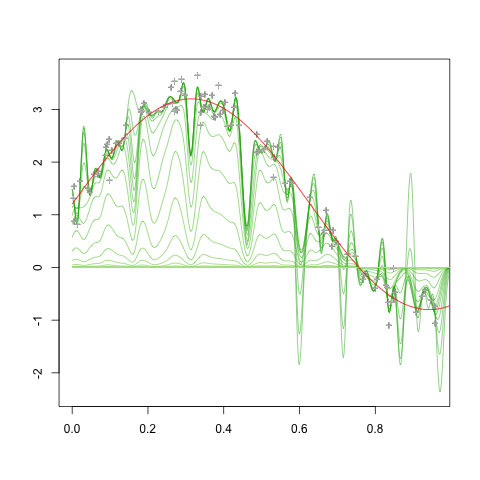
\includegraphics[scale=0.5]{PS_penalty_section_figure_6_order_0.png}
  %\label{fig:pspline_small_lambda}
\caption{$d=0$ }
\end{subfigure}
\begin{subfigure}{.5\textwidth}
  \centering
   \graphicspath{{img/}}
  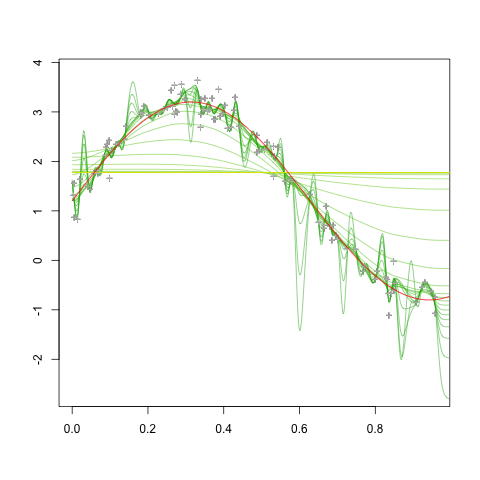
\includegraphics[scale=0.5]{PS_penalty_section_figure_6_order_1.png}
 % \label{fig:pspline_small_lambda}
\caption{$d=1$}
\end{subfigure}
\begin{subfigure}{.5\textwidth}
  \centering
   \graphicspath{{img/}}
  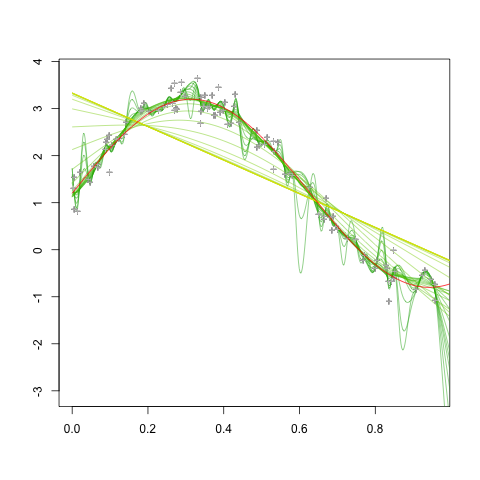
\includegraphics[scale=0.5]{PS_penalty_section_figure_6_order_2.png}
  %\label{fig:pspline_small_lambda}
\caption{$d=2$}
\end{subfigure}
\begin{subfigure}{.5\textwidth}
  \centering
   \graphicspath{{img/}}
  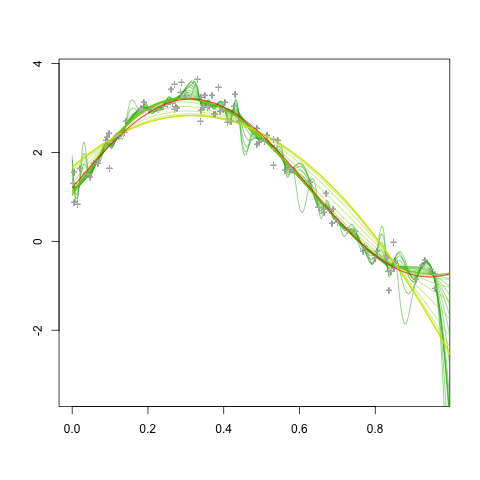
\includegraphics[scale=0.5]{PS_penalty_section_figure_6_order_3.png}
  %\label{fig:pspline_small_lambda}
\caption{$d=3$}
\end{subfigure}
\caption{\textit{Illustration of the impact of the order of the difference penalty. The number of B-splines used is the same in each plot, with the penalty parameter varying from across the same grid of values. The fitted curves in the upper left plot correspond to the difference penalty of order $0$, where $\vert D_0 \alpha \vert^2 = \sum_{i=1}^n \alpha_i^2$, analogous to ridge regression using the B-spline basis as regression covariates. The fitted curves approach polynomials of degree $d-1$ as $\lambda \rightarrow \infty$, as discussed in \ref{eq:PS_properties} \ref{eq:PS_property_3}.}}
\label{fig:PS_penalty_section_figure_6}
\end{figure}

\begin{figure}[h]
\centering
 \graphicspath{{img/}}
  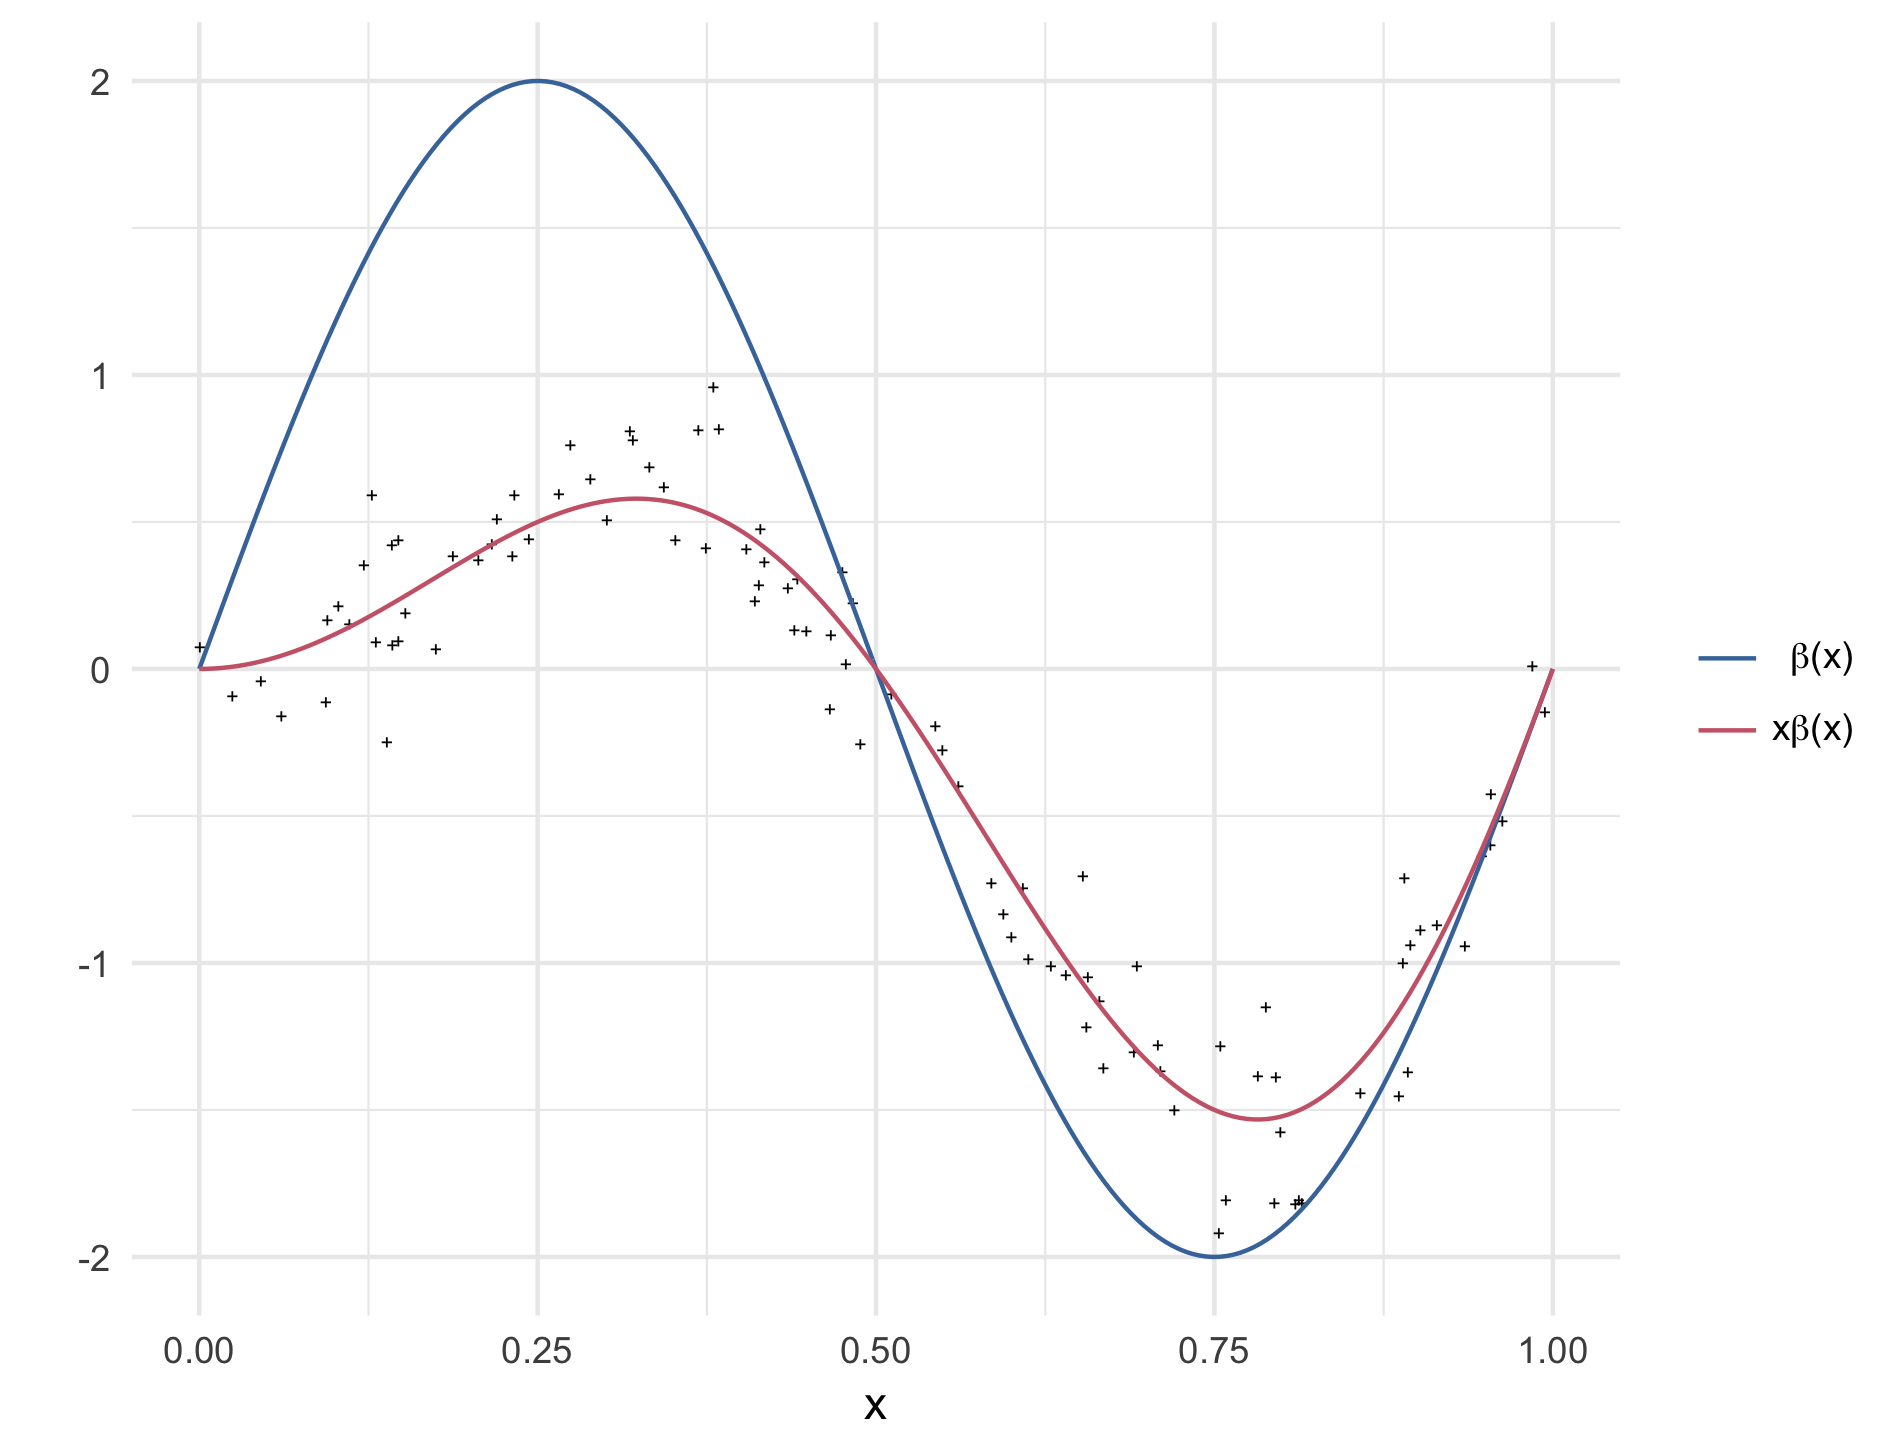
\includegraphics[width=4in, height=4in]{PS_penalty_section_figure_5.png}
 %\caption{Tensor product of two cubic B-splines}
\end{figure}

\section{Estimating $\phi$ via penalized maximum likelihood}

We employ maximum likelihood  for the estimation of  the varying coefficient function $\phi\left(t,s\right)$ and the innovation variance function $\sigma\left(t\right)$, though neither the derivation the form of model~\ref{eq:ARmodel} nor model~\ref{eq:MyModel} via the Cholesky decomposition rely on any assumptions about the distribution of $Y$. 

For fixed $\left\{ \sigma_j^2 \right\}$, as a function of $\phi_{jk}$ the negative log-likelihood for a sample of $N$  i.i.d. observations $Y_1,Y_2,\dots,Y_N$ from a multivariate Gaussian distribution is proportional to the usual error sums of squares:

\begin{equation}
-2 L\left(y_1,\dots,y_N ,\phi^* \vert \vsigmasq \right) \propto \sum_{i=1}^N \sum_{j=2}^{m_i} \sigma\left({t_j}\right)^{-2} \left(y_{ij} - \sum_{k=1}^{j-1}\phi\left({t_{ij},t_{ik}}\right)y_{ik} \right)^2 \label{loglikelihood}
\end{equation}
\noindent
where 
\[
y_i = \left( y_{i1}, y_{i2}, \dots, y_{i,m_i}\right), \quad i=1,\dots,N 
\] 

%% explain here that we omit y_{i1} from the likelihood here because in the first stage of estimation (for $\phi$), the first observation in each vector doesn't contribute to the likelihood
\noindent
denotes the vector of observations for subject $i$ with corresponding measurement times 
\[
t_{i1} < t_{i2} < \dots < t_{i,m_i}.
\]
The form of the likelihood of $y_1,\dots,y_N$ indicates that we allow both the number of measurements as well as the observation times to varying across subjects. The $\left\{t_{ij} \right\}$ need not be evenly-spaced within or across individuals. Denote the innovation variance function evaluated at the vector of observed time points by $\vsigmasq$, and similarly let $\vphistar$ denote the resulting vector when evaluating $\phi^*$ at the observed grid of time points, transformed to the $l$-$m$ axis. Estimation of the varying coefficient function and the innovation variance function may be accomplished in an iterative fashion:

\fbox{\parbox{\textwidth}{\begin{enumerate}
\item Fix $\vsigmasq = \vsigmasq_0$;
\item find $\widehat{\vphistar} = \underset{\vphistar}{\arg\max} -2 L\left(y_1,\dots,y_N ,\vphistar \vert \vsigmasq_0 \right)$.
\item Fix $\vphistar= \widehat{\vphistar}$;
\item find $\widehat{\vsigmasq} = \underset{\vsigmasq}{\arg\max} -2 L\left(y_1,\dots,y_N , \vsigmasq \vert \widehat{\vphistar} \right)$.
\item Iterate until convergence.
\end{enumerate}}}

\vspace{0.5cm}




% 
%\section{\emph{Penalized maximum likelihood estimation}}
%
%\begin{enumerate}
%\item Fix $\sigma_{ij}^2 = \sigma_{ij0}^2$, $i=1,\dots,N$ ,$j=1,\dots,M$.
%\item Find $\phi_0 = \underset{\phi}{arg \; min} -2L_\phi\left(\phi, y_1,\dots, y_N \right) + \lambda J\left( \phi \right)$
%\item Fix $\phi = \phi_{0}$.
%\item Find  $\sigma_{0}^2 = \underset{\sigma^2}{arg\; min} -2L_\sigma^2\left(\sigma^2, y_1,\dots, y_N \right) + \lambda J\left( \sigma^2 \right)$
%\end{enumerate}
%
%\begin{adjustwidth}{-2cm}{-2cm}
%\begin{equation}
%-2 L_\phi\left(\phi, y_1, \dots,y_N \right) = \sum_{i=1}^N \sum_{j=2}^{m_i} \sigma_{ij0}^{-2} \left(y_{ij} - \sum_{k=1}^{j-1}\phi\left({t_{ij},t_{ik}}\right)y_{ik} \right)^2 \label{loglikelihood}
%\end{equation}
%\end{adjustwidth}
% 





% 
%\section{\emph{Smooth ANOVA models}}
%Decompose
%\begin{equation} \label{eq:SANOVA-model}
%\carrotorangemath{
%\phi^*\left(l,m\right) = \mu + \phi_1\left(l\right) + \phi_2\left(m\right) + \phi_{12}\left(l,m\right)},
%\end{equation} 
%so Model~\ref{eq:MyModel} becomes
%
%\begin{align*}  
%\begin{split}% \label{eq:expanded-ps-anova-vc-model}
% y\left(t_j \right)  = \sum_{k=1}^{j-1} \bigg[\mu + \phi_1\left(l_{jk}\right) +  &\phi_2\left(m_{jk}\right) \bigg.\\[-2ex]
%\bigg. &+ \phi_{12}\left(l_{jk},m_{jk}\right) \bigg]y\left(t_k\right)+ \sigma\left(t_j\right)e\left({t_j}\right)
%\end{split}
%\end{align*}
% 
%

 

%
% \begin{columns}
%\begin{column}{0.5\textwidth}
%Equip $l$ and $m$ with
%\begin{align*}
%B_{1}\left(l\right),\dots, B_{K}\left(l\right),\\
%B_{1}\left(m\right),\dots, B_{L}\left(m\right)
%\end{align*}
%to build
%\begin{equation*}
%T_{jk}\left(l,m\right) = B_j\left(l\right){B}_k\left(m\right)
%\end{equation*}
%  \end{column}
%\begin{column}{0.5\textwidth}  %%<--- here
%    \begin{center}
%    \begin{figure}
%    \graphicspath{{img/}}
% 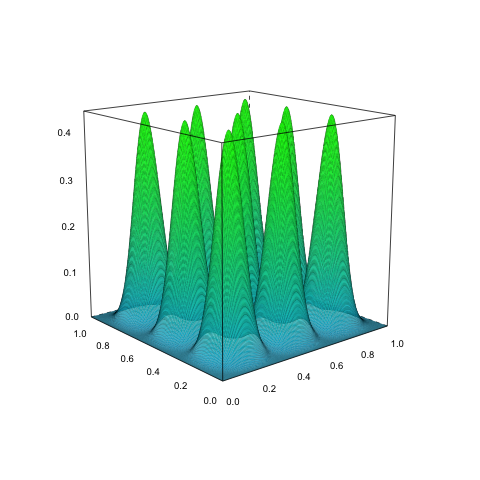
\includegraphics[width=4cm]{sparse_bicubic_basis}
% \caption{A ``thinned'' tensor product basis}
% \end{figure}
%     \end{center}
%\end{column}
%\end{columns}
%\vspace{0.3cm}
%\begin{equation*}
%\phi^*\left(l,m\right) = \sum_{i=1}^K \sum_{j=1}^L \theta_{ij} B_{i}\left(l\right) B_{j}\left(m\right)
%\end{equation*}
%
 



%The parameters of the functional autoregressive model given by \ref{eq:MyModel} define the elements of the precision matrix $\Omega$, rather than the elements of $\Sigma$ itself. It is well known that if we let $Y = \left(Y_1, \dots, Y_m\right)^\prime$ denote the random vector having joint distribution with mean zero and covariance matrix $\Sigma$, then the elements of $\Sigma^{-1}=\Omega$, $\left\{ \omega_{ij} \right\}$ may be interpreted as partial covariances between the elements of $Y$. This suggests shrinking $\phi^*$ to zero for large values of $l$. One can show that if $T$ has $k$ non-zero diagonals, then the middle $k$ diagonals of $\Sigma^{-1}$ are non-zero.  


For ease of exposition, we first focus our attention on the estimation of $\phi$ assume that $\sigma^2\left(t\right)$ is fixed and known. Estimation of the innovation variance function is presented in Section~\ref{section:variance-estimation}. In the case that subjects share a common set of observation times $t_1 < \dots < t_m$,  it is well known that the MLE for $\Sigma$, $S = \sum_{i=1}^N y_i y_i^\prime$ is highly unstable in high dimensions, a condition that is potentially worsened when one or more subjects has at least one observation time that is unique from the set of observation times common across subjects. To mitigate instability due to high dimensionality and simultaneously permit the estimation of $\phi\left(\cdot,\cdot\right)$ as a smooth bivariate function, we obtain a covariance estimator by applying bivariate smoothing of the elements of the Cholesky factor. 

Estimating the varying coefficient function $\phi^*$, however, is quite different from the usual problem of estimating an arbitrary bivariate function. In the case of the latter, we most typically treat both arguments equally in terms of regularization, but in the case of covariance estimation and the generalized coefficient function equal treatment of $l$ and $m$ in terms of penalization perhaps is not the most appropriate approach. The lag component, $l$, has particularly significant meaning in terms of the covariance function and thus also in terms of $\phi^*$ and is of considerable more interest than the orthogonal component, $m$. We parameterize $\phi$ in terms of the transformed domain:

\begin{align*}
l = t-s, \qquad m = \frac{1}{2}\left(s+t\right),
\end{align*}
\noindent
so that the following relationship holds:
\begin{align*}
\phi\left(s,t\right) = \phi^*\left(s-t, \frac{1}{2}\left(s+t\right)\right) =\phi^*\left(l,m\right)
\end{align*}
with 
\begin{equation} \label{eq:phi-star-domain}
\frac{l}{2} < m < 1 - \frac{l}{2}, \quad 0 < l < 1.
\end{equation}

\noindent
The likelihood can be written in terms of the reparameterized varying coefficient function:

\begin{align} 
\begin{split} \label{loglikelihood}
-2L\left(y_1,\dots,y_N ,\phi^* \vert \vsigmasq \right) &= \sum_{i=1}^n \sum_{j=2}^{m_i} \sigma_{ij}^{-2} \left(y_{ij} - \sum_{k=1}^{j-1}\phi\left({t_{ij},t_{ik}}\right)y_{ik} \right)^2 \\
&= \sum_{i=1}^n \sum_{j=2}^{m_i} \sigma_{ij}^{-2} \left(y_{ij} - \sum_{k=1}^{j-1}\phi^*\left({l_{ijk},m_{ijk}}\right)y_{ik} \right)^2 
\end{split} 
\end{align}

We equip the $l$ and $m$ axes each with a B-spline basis to construct a basis for the varying coefficient function $\phi$ in \ref{eq:phi-star} by taking the tensor product of the two marginal bases. Let 
\[
B_{1}\left(l\right),\dots, B_{K}\left(l\right)  \mbox{ and } B_{1}\left(m\right),\dots, B_{L}\left(m\right)
\]
denote the B-spline bases for $l$ and $m$, each having a set of equally spaced knots along their respective domain. It is worth noting that while we have chosen not to distinguish between $\left\{ B_k \right\}$ and $\left\{ {B}_l \right\}$ for the sake of brevity, one is free to specify a different basis for each dimension either by using different order B-spline or, of course, using different numbers of knots, and hence entirely different knot sequences since P-splines rely on bases with equally spaced knots. The tensor product basis functions
\begin{equation*}
T_{jk}\left(l,m\right) = B_j\left(l\right){B}_k\left(m\right)
\end{equation*}
\noindent
carve the $l$-$m$ domain into rectangles.  Figure~\ref{fig:sparse_bicubic_BS_basis} shows a thinned tensor product basis $\left\{ T_{kl} \right\}$; a portion of the basis was omitted to eliminate overlapping of the basis functions so that the reader can identify individual tensor products. Each ``hill'' in Figure~\ref{fig:sparse_bicubic_BS_basis} is associated with an unknown coefficient $\theta_{ij}$ which determines the height of the hill. For a given knot grid, we can approximate a surface by

\begin{equation} \label{eq:varying-coefficient-tensor-product-expansion}
\phi^*\left(l,m\right) = \sum_{i=1}^K \sum_{j=1}^L \theta_{ij} B_{i}\left(l\right) B_{j}\left(m\right), 
\end{equation}
\noindent
and the function evaluated at the observed $\left(l_{ijk}, m_{ijk}\right)$ may be written 
\begin{equation*} 
\vphistar = B_m \Theta B_l^\prime
\end{equation*}
\noindent 
where $\Theta$ denotes the $K \times L$ matrix of tensor product coefficients, with elements $\theta_{ij}$.

\begin{figure}[H]
\centering
 \graphicspath{{img/}}
  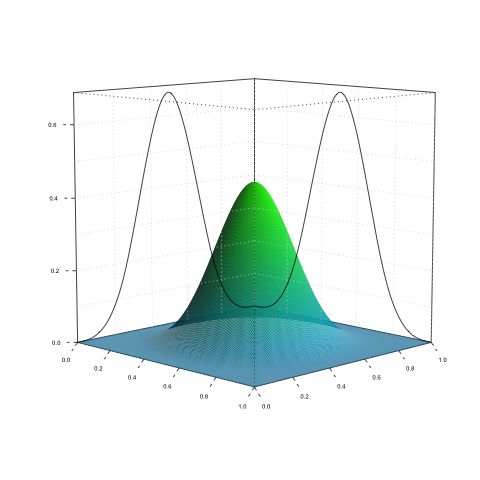
\includegraphics[width=4in, height=4in]{bicubic_basis_function.png}
 
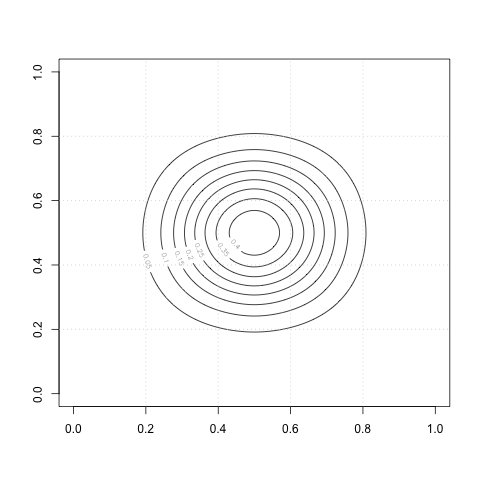
\includegraphics[width=4in, height=4in]{bicubic_bspline_contour.png}
\caption{Tensor product of two cubic B-splines}
\label{fig:bicubic_BS}
\end{figure}

\begin{figure}[H]
  \centering
  \graphicspath{{img/}}
  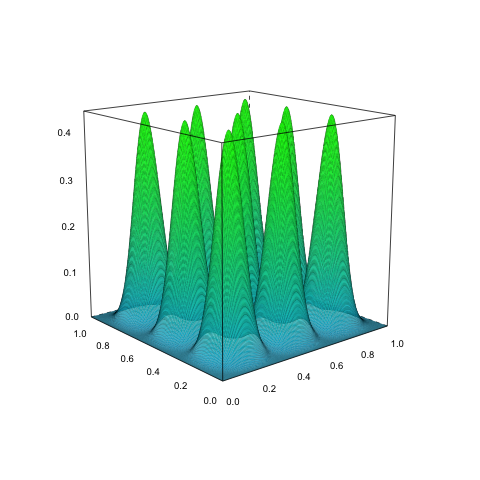
\includegraphics[width=5in,height=5in]{sparse_bicubic_basis.png}
  \caption{A subset of a full bivariate basis of cubic B-splines}\label{fig:sparse_bicubic_BS_basis}
\end{figure}

\subsection{Regularization with difference penalties} \label{subsection:univariate-psplines}

The minimizer of \ref{eq:loglikelihood} honors the fidelity to the data, so to balance the complexity of the fitted function with the goodness of fit to the data, we can append a penalty to the negative log likelihood to control the fitted function. By using rich B-spline bases for $l$ and $m$ alongside discrete difference penalties on the spline coefficients, we can achieve as much smoothness of the fitted function in both the $l$ and $m$ dimensions as desired. \citet{o1986statistical} was the first to propose using a rich B-spline basis and using a penalty to restrict the flexibility of the fitted curve, like \citet{wahba1990spline} applying a penalty to the second derivative of the fitted curve:
\[
J = \int_0^1 \left[ f^{\prime \prime}\left(l\right)\right]^2\;dx.
\]

For a B-spline of the form
\[
f\left(x\right) = \sum\limits_{j=1}^n \theta_i B_j\left(x\right),
\]
one can derive a banded matrix $P$ using the properties of B-splines such that 
 \[
 J = \theta^\prime P \theta
 \] 
 \noindent
 where $\theta = \left(\theta_1,\dots, \theta_n\right)$. The $i$-$j^{th}$ element of $P$ is given by
 \[
 p_{ij} = \int_0^1 B_i^{\prime \prime} \left( x \right)B_j^{\prime \prime} \left( x \right)\;dx.
 \]

%As discussed in Section 2, we can define an entire class of functional autoregressive models using only the $l$ direction, and additionally, as discussed in Section 3, there is a natural expectation about the functional form of the autoregressive coefficient function (and hence covariance) as a function of $l$. The use of smoothing splines to estimate $\phi$ outlined in Section~\ref{} yields smooth null models, but smoothness of the elements of the Cholesky factor alone may not lead to desirable structure in the inverse covariance matrix.  

%
%These approaches implicitly adopt different notions of sparsity. Like \citet{huang2006covariance} and \citet{levina2008sparse}, our aim is to regularize the inverse of the covariance matrix through the Cholesky factor. Expressing the varying coefficient function using a tensor product basis expansion builds the foundation for a flexible estimation framework within which employing multiple notions of smoothness is simple and straightforward. 
%

In some applications, it is useful to work with third and fourth order differences, since for large values of $\lambda$, the fitted curve approaches a parametric polynomial model. This may be of particular interest in the context of estimating the elements of the Cholesky factor, as many have proposed simple parametric functions of lag only for $\phi^*$, such as low order polynomials. See \citet{pourahmadi1999joint}. However, with the use of higher order derivatives, the computation of $P$ is nontrivial and becomes very tedious. \citet{eilers1996flexible} were the first to propose P-splines, or \emph{penalized B-splines}, as an approach to nonparametric regression. P-splines circumvent complexity associated with constructing such penalty matrices by omitting derivatives and integrals altogether, replacing them with finite differences and sums. 

Instead, flexibility of the fitted function is controlled by using a discrete penalty matrix based on finite difference formulas. Smoothness of the fitted function is achieved by first using a rich B-spline basis with equally spaced knots to purposefully overfit the smooth coefficient vectors; this eliminates the difficulty of choosing the optimal set of knots. Then by attaching a difference penalty to the goodness of fit measure, one may prevent overfitting and make a potentially ill-conditioned fitting procedure a well-conditioned one. The finite difference penalty is simple to compute and can be handled mechanically for any order of the differences. Since it is easily introduced into regression equations, it is feasible to evaluate the impact of different orders of the differences on the fitted model.  Using the properties of B-splines, it is straightforward to show that the difference penalty of order $d$ is a good discrete approximation to the integrated square of the $d^{th}$ derivative, so little is lost by replacing the derivative-based penalty with

\begin{equation} \label{eq:bspline-difference-penalty}
J_d\left( f \right) = \sum_{j=d}^n \left(\Delta^d \theta_j\right)^2
\end{equation} 
\noindent
where $\theta = \left( \theta_1,\dots,\theta_n \right)$. Let $D_d$ denote the matrix difference operator: $D_d\theta = \Delta^d \theta$, where

 \begin{align*}
 \Delta \theta_j &= \theta_j - \theta_{j-1}, \quad  \Delta^2 \theta_j = \Delta\left(\Delta \theta_j\right) = \theta_j - 2\theta_{j-1} + \theta_{j-2}
 \end{align*}
\noindent 
In general,
\begin{equation*}
\Delta^d \theta_j = \Delta\left(\Delta^{d-1} \theta_j \right).
\end{equation*} 
\noindent
Then, \ref{eq:bspline-difference-penalty} can be written in terms of the squared norm of the difference operator applied to the vector of B-spline coefficients:
\begin{align} 
\begin{split} \label{eq:bspline-difference-penalty-vector-form}
J_d\left( f \right) &= \vert \vert D_d\theta \vert \vert^2 \\
&= \theta^\prime P_d \theta
\end{split}
\end{align}
\noindent
where $P_d = D_d^\prime D_d$.  To examine the connection between the second-derivative penalty to the penalty on second-order differences of the B-spline coefficients, we only need to employ straightforward calculus and exploit the recursive property of the B-spline basis functions:

\begin{equation*} 
\int_0^1 \left[ f^{\prime \prime}\left(x\right)\right]^2\;dx = \int_{0}^{1} \left\{ \sum\limits_{j=1}^n  \theta_j B_{j,3}^{\prime \prime} \left(l\right) \right\}^2\; dl.
\end{equation*}
\noindent
The derivative properties of B-splines permits this to be written as 
\begin{equation*} \label{eq:second-derivative-bspline-penalty}
\int_0^1 \left[ f^{\prime \prime}\left(x\right)\right]^2\;dx =  \int_{0}^{1}  \bigg[ \sum\limits_{j=1}^n \sum\limits_{k=1}^n \Delta^2 \theta_j \Delta^2 \theta_k B_{j,1}\left(l\right)B_{k,1}\left(l\right)\bigg]\; dl  . 
\end{equation*}
\noindent
Most of the cross products of $B_{j,1}\left(x\right)$ and $B_{k,1}\left( x \right)$ vanish since B-splines of degree 1 only overlap when $j$ is $k-1$, $k$, or $k+1$. Thus, we have that
\begin{align}
\begin{split}
\int_0^1 \left[ f^{\prime \prime}\left(x\right)\right]^2\;dx  = {} &  \int_0^1 \bigg[ \left\{ \sum\limits_{j=1}^n   \Delta^2 \theta_j  B_j\left(l,1\right)  \right\}^2  + 2 \sum_{j}\Delta^2 \theta_j\Delta^2 \theta_{j-1}B_j\left(l,1\right)B_{j-1}\left(l,1\right) \bigg]\; dl \\ 
= {} & \sum \limits_{j=1}^n  \left( \Delta^2\theta_j \right)^2 \int_0^1 B_j^2\left(l,1\right)\;dl \\
   &{} \;\;\;\;\;\;\;\;\;\;\;\;\;\;\;\;\;\; + 2 \sum\limits_{j=1}^n \Delta^2 \theta_j\Delta^2 \theta_{j-1} \int_0^1 B_j\left(l,1\right)B_{j-1}\left(l,1\right)\;dl 
\end{split}
\end{align}
\noindent
which can be written as
\begin{equation} \label{eq:derivative-penalty-difference-penalty-connection}
\int_0^1 \left[ f^{\prime \prime}\left(x\right)\right]^2\;dx  = c_1 \sum\limits_{j=2}^n \left( \Delta^2 \theta_j\right)^2 + c_2 \sum\limits_{j=3}^n \Delta^2 \theta_j\Delta^2 \theta_{j-1}
\end{equation}
\noindent
Given a set of equidistant knots, the constants $c_1$ and $c_2$ are given by
\begin{equation}
\begin{split}
c_1 & =   \int_0^1 B_{j,1}^2\left(x\right) dx\\
c_2 & = \int_0^1 B_{j,1}\left(x\right)B_{j-1,1}\left(x\right) dx.
\end{split}
\end{equation}

This gives us that the traditional smoothness penalty on the squared second derivative can be written as a linear combination of a penalty on the second-order differences of the B-spline coefficients \ref{eq:bspline-difference-penalty} and the sum of the cross products of neighboring second differences. The second term in \ref{eq:derivative-penalty-difference-penalty-connection} leads to a complex objective function when minimizing the penalized likelihood, where seven adjacent spline coefficients occur, as opposed to five if only the first term in \ref{eq:derivative-penalty-difference-penalty-connection} is used in the penalty. The added complexity is a consequence of overlapping B-splines, which quickly increases when using higher order differences and higher order B-splines. We can seamlessly augment the likelihood with the difference penalty to achieve smooth fitted functions without the complexity posed by the derivative-based penalty.
%citet{chen2011efficient}, citet{pourahmadi1999joint}, and citet{pourahmadi2002dynamic} have elicited parametric models for the generalized autoregressive coefficients, letting the GARPs depend only on the distance between two time points.

A smoother sequence of coefficients leads to a smoother curve, as illustrated in Figure~\ref{fig:second_ord_PS_pen_SML_lambda}.  The relationship between P-spline curves and their coefficients is easily characterized if we consider the coefficients as the skeleton of the function, and draping the B-splines over them puts the flesh on the bones. As long as the coefficient sequence is smooth, the number of basis functions (and coefficients) is unimportant since the penalty ensures the smoothness of the skeleton and that the fitting procedure is well-conditioned. Figure~\ref{fig:overcomplete_basis_pspline} illustrates this utility of the penalty for simulated data; there are $m=10$ observations and $60$ cubic B-splines. This property of P-splines cannot be overly appreciated because it frees us from the concern of choosing the optimal set of knots. Unless computational constraints are of concern, which is possible with large models, it is prudent to use even more B-splines. Figure~\ref{fig:PS_penalty_section_figure_2} shows how the fitted function changes as the tuning parameter varies when the data are sparsely sampled. P-splines enjoy a number of additional advantageous properties, many of which are inherited from the attractive properties of B-splines. See \citet{eilers1996flexible}  for a detailed presentation. 

\begin{figure}[H] \label{fig:PS-smoothing-figure-1}
\begin{subfigure}{.5\textwidth}
  \centering
   \graphicspath{{img/}}
  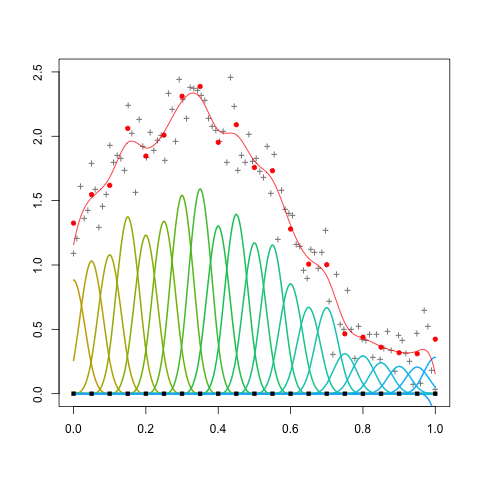
\includegraphics[scale=0.5]{pspline_pord2_xsmall_lambda.png}
  \label{fig:pspline_small_lambda}
\end{subfigure}
\begin{subfigure}{.5\textwidth}
  \centering
   \graphicspath{{img/}}
  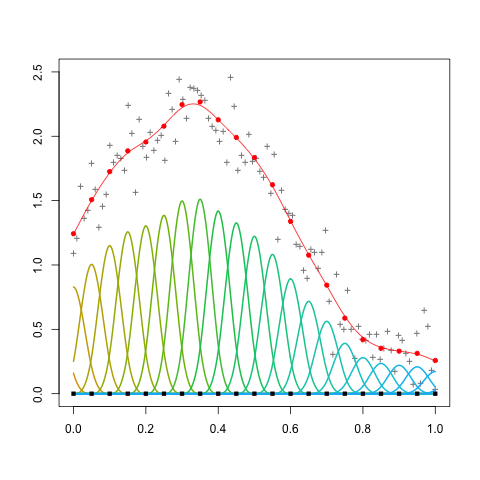
\includegraphics[scale=0.5]{pspline_pord2_small_lambda.png}
  \label{fig:pspline_small_lambda}
\end{subfigure}
\begin{subfigure}{.5\textwidth}
  \centering
   \graphicspath{{img/}}
  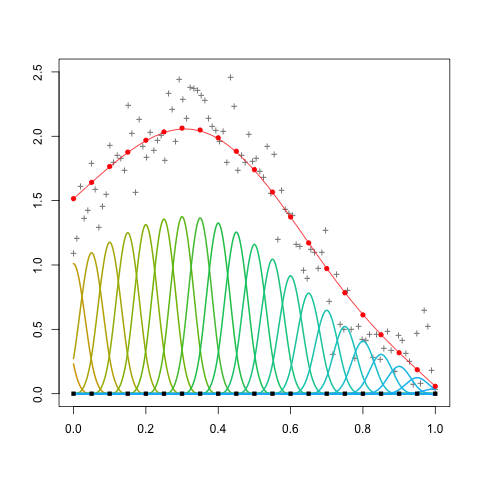
\includegraphics[scale=0.5]{pspline_pord2_medium_lambda.png}
  \label{fig:pspline_small_lambda}
\end{subfigure}
\begin{subfigure}{.5\textwidth}
  \centering
   \graphicspath{{img/}}
  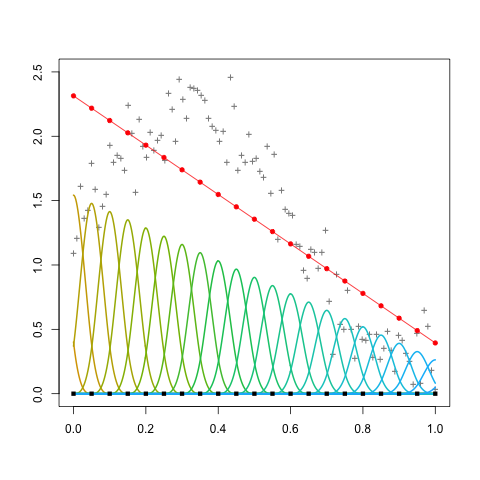
\includegraphics[scale=0.5]{pspline_pord2_large_lambda.png}
  \label{fig:pspline_small_lambda}
\end{subfigure}
\caption{\textit{Illustration of the impact of the second order difference penalty. The number of B-splines used is the same in each plot, with the value of the penalty parameter increasing from left to right and top to bottom across each plot. The fitted curve in the upper left plot is the most ``wiggly'' of any of the fits, as the penalty plays the weakest roll in the fitted coefficients there. The red circles are the values of each of the B-spline coefficients; as the penalty increases, they form as smoother sequence as we move across the four plots, which results in a smoother fitted function. As the penalty parameter approaches infinity, the fit approaches a linear function as shown in the bottom right plot.}}
\label{fig:second-ord-PS-pen-SML-lambda}
\end{figure}


%First, unlike many types of kernel smoothers, P-splines show no boundary effects i.e. the spreading of the fitted curve outside of the physical domain of the data, usually while also bending toward zero. See \citet{eilers1996flexible} Section 8 for a detailed discussion.

%P-splines can fit polynomial data exactly. Given data $\left(l_i,y_i\right)$, if the $y_i$ are a polynomial in $l$ of degree $k$, then B-splines of degree $k$ or higher will fit the data exactly.  The same is true for P-splines if the order of the penalty is $k+1$ or higher, irrespective of the value of $\lambda$. An informal proof is left to the appendix.
%
%Under a difference penalty of order $k$, the fitted function will approach a polynomial of degree $k-1$ for large values of $\lambda$ as long as the degree of the B-splines is greater than or equal to $k$. This can be shown by once again considering the relationship between the derivatives of a B-spline fit and the differences in neighboring coefficients; detailed discussion is left to the appendix. Figure~\ref{fig:PS_penalty_section_figure_6} visually demonstrates this property by examining the behavior of the fitted function as the tuning parameter varies under a difference penalty of order $d=0,1,2,3$.
%
%We will leverage several properties of the smoothing matrix, $H$, for model evaluation and selection, so focus on the linearized smoothing problem solved at each value of the penalty parameter, $\lambda$, is prudent. The trace of $H$ approaches the order of the differencing operator, $k$ for larges values of $\lambda$. The trace of the smoothing matrix is a useful measure of effective model dimension, so understanding its limiting behavior is important. 



To extend these results to the bivariate setting for regularizing of $\phi^*$, the only modification to the differencing procedure in one dimension necessary is the addition of a second difference penalty, one for each variable $l$ and $m$. We append the pair of penalties to the negative log likelihood \ref{eq:loglikelihood} and take the estimator of $\phi^*$ to correspond to the B-spline coefficients minimizing

\begin{align} 
\begin{split}\label{eq:unfolded-difference-penalty-log-likelihood}
-2L + J\left(\phi^*\right) = \sum_{i=1}^N \sum_{j=2}^{m_i} \sigma\left({t_j}\right)^{-2} \left\{y_{ij} - \sum_{k=1}^{j-1} \left( \sum_{r=1}^L \sum_{s=1}^K \theta_{rs} B_r\left(l_{ijk}\right)B_s\left(m_{ijk}\right)\right)y_{ik} \right\}^2 \\ 
+ \lambda_l \sum_{r^\prime=1}^K \vert D_{d_{\ms l}} \theta_{r^\prime \cdot} \vert^2 + \lambda_m \sum_{s^\prime=1}^L \vert D_{d_{\ms m}} \theta_{\cdot s^\prime} \vert^2.
\end{split}
\end{align}


%\begin{align*}\label{eq:unfolded-row-column-difference-penalty}
%\mathcal{Q}=\sum_{i=1}^n \sum_{j=2}^{m_i} \sigma_{ij}^{-2} \left[y_{ij} - \sum_{k=1}^{j-1}\left(\sum_{i=1}^K \sum_{j=1}^L \theta_{ij} B_{i}\left(l_{ijk}\right) B_{j}\left( m_{ijk} \right)  \right) y_{ik} \right]^2 \\
%\mbox{\;\;\;\;\;\;\;\;}+ \lambda_l \sum_{k} \vert D_d \theta_{k \cdot} \vert^2 + \lambda_m \sum_{l} \vert D_{\ms d_{\ms m}} \theta_{\cdot l} \vert^2 
%\end{align*}

\noindent
where $\theta_{k \cdot}$ and $\theta_{\cdot l}$ denote the $k^{th}$ row and $l^{th}$ column of $\Theta$, respectively. The first term in\ref{eq:unfolded-row-column-difference-penalty} imposes a difference penalty of order $d_{\ms l}$ on the rows of the coefficient matrix while the second term places a difference penalty (of possible different order $d_{\ms m}$) on the columns. We give each direction its own smoothing parameter to permit anisotropic smoothing; however, one could opt to use a single smoothing parameter for both directions and dodge the added work of optimizing the amount of smoothing with two separate parameters. Figure ~\ref{fig:2d_PS_penalty_demo} shows a potential result of heavy column penalization (left) and heavy row penalization (right) under a second order difference penalty on each row and each column for large values of $\lambda_l$ and $\lambda_m$. The figure demonstrates that the limiting behaviour of each row and column is linear, but the resulting surface may exhibit slope reversals from one row (column) to the next. 


\begin{figure}[H] \label{fig:2d_PS_penalty_demo}
 \begin{subfigure}{.48\textwidth}
  \centering
   \graphicspath{{img/}}
 \includegraphics[scale=0.5]{"model selection/effective dimension/2d_PS_section_figure1_big_col_lambda"}
 \caption{\textit{heavy column penalty}}
 \label{fig:2D_PS_big_col_penalty}
 \end{subfigure}
 \begin{subfigure}{.48\textwidth}
  \centering
   \graphicspath{{img/}}
  \includegraphics[scale=0.5]{"model selection/effective dimension/2d_PS_section_figure1_big_row_lambda"}
 \caption{\textit{heavy row penalty}}
\label{fig:2D_PS_big_row_penalty}
 \end{subfigure}
 \caption{\textit{Nine cubic B-spline tensor products with heavy linear column penalty and heavy linear row penalty}}
\end{figure}
\noindent
We take the estimator of $\phi^*$ to be the minimizer of 
It is computationally advantageous to express the coefficient matrix in ``unfolded'' notation, which allows us to express the varying coefficient function at the observed coordinate grid as in the usual multiple regression form:

\begin{equation*}
\mbox{vec}\left\{\phi^*\left(l,m\right)\right\} = B \theta
\end{equation*}
\noindent
Stacking the columns of $\Theta$ gives the vectorized coefficient matrix $\theta = \mbox{vec}\left( \Theta \right)$. The $p \times KL$ tensor product basis $B$ is constructed from the tensor product of the marginal B-spline bases defined in \citet{eilers2006fast} as the \textit{row-wise Kronecker product} of the individual bases:

\begin{equation} \label{eq:rowwise-kronecker-product}
B = B_l \square B_m = \left( B_m \otimes 1^\prime_{K} \right) \odot \left(1^\prime_{L} \otimes  B_l  \right).
\end{equation}
\noindent
The operator $\odot$ denotes the element-wise matrix product; $1_K$ ($1_L$) denotes the column vector of ones having length $K$ ($L$.) The operations in \ref{eq:rowwise-kronecker-product} construct $B$ such that the $i^{th}$ row of $B_m\square B_l$ is the Kronecker product of the corresponding rows of $B_m$ and $B_l$. The penalty in \ref{eq:unfolded-row-column-difference-penalty} can also be compactly expressed:

\begin{equation*} \label{eq:tensor-product-penalty}
\lambda_l \vert \vert P_l \theta \vert \vert^2 + \lambda_m \vert \vert P_m \theta \vert\vert^2
\end{equation*}

where $P_l = I_L \otimes D_{d_{\ms l}}^\prime D_{d_{\ms l}} $ and $P_m =  D_{d_{\ms m}}^\prime D_{d_{\ms m}} \otimes I_K$. We define the matrix $W$ of historical regressors so that \ref{eq:unfolded-difference-penalty-log-likelihood} can be written in matrix form as

\begin{equation} \label{eq:tensor-pspline-objective-function}
-2L + J\left(\phi^*\right) = \left( Y - WB\theta\right)^\prime D^{-1}\left( Y - WB\theta\right)  + \lambda_l \vert\vert P_l \theta \vert\vert^2 + \lambda_m \vert\vert P_m \theta\vert \vert^2,
\end{equation}
\noindent
with $\hat{\theta}$ solving the system of equations 
\begin{equation} \label{eq:tensor-pspline-normal-equations}
\left[ \left(WB\right)^\prime D^{-1} WB +  \lambda_l P_l+ \lambda_m P_m\right]\theta = \left(W B\right)^\prime D^{-1}Y
\end{equation}
\noindent
From \ref{eq:tensor-pspline-normal-equations}, we note that the system of equations depends on basis coefficients remains fixed at $KL$, even as the number of observations increases.   The grid of regression coefficients can be recovered by arranging the elements of $\hat{\theta}$ into a matrix of $L$ columns having length $K$. 

This recipe for constructing a tensor product basis for $\phi^*$ is an easy and convenient way to construct a two-dimensional basis for a bivariate function with domain corresponding to the unit square. However, the domain of the autoregressive coefficient function, specified in \ref{eq:phi-star-domain}, lies on the lower triangle of the unit square:

\begin{figure}[H] \label{fig:triangle-domain}
    \graphicspath{{img/}}
 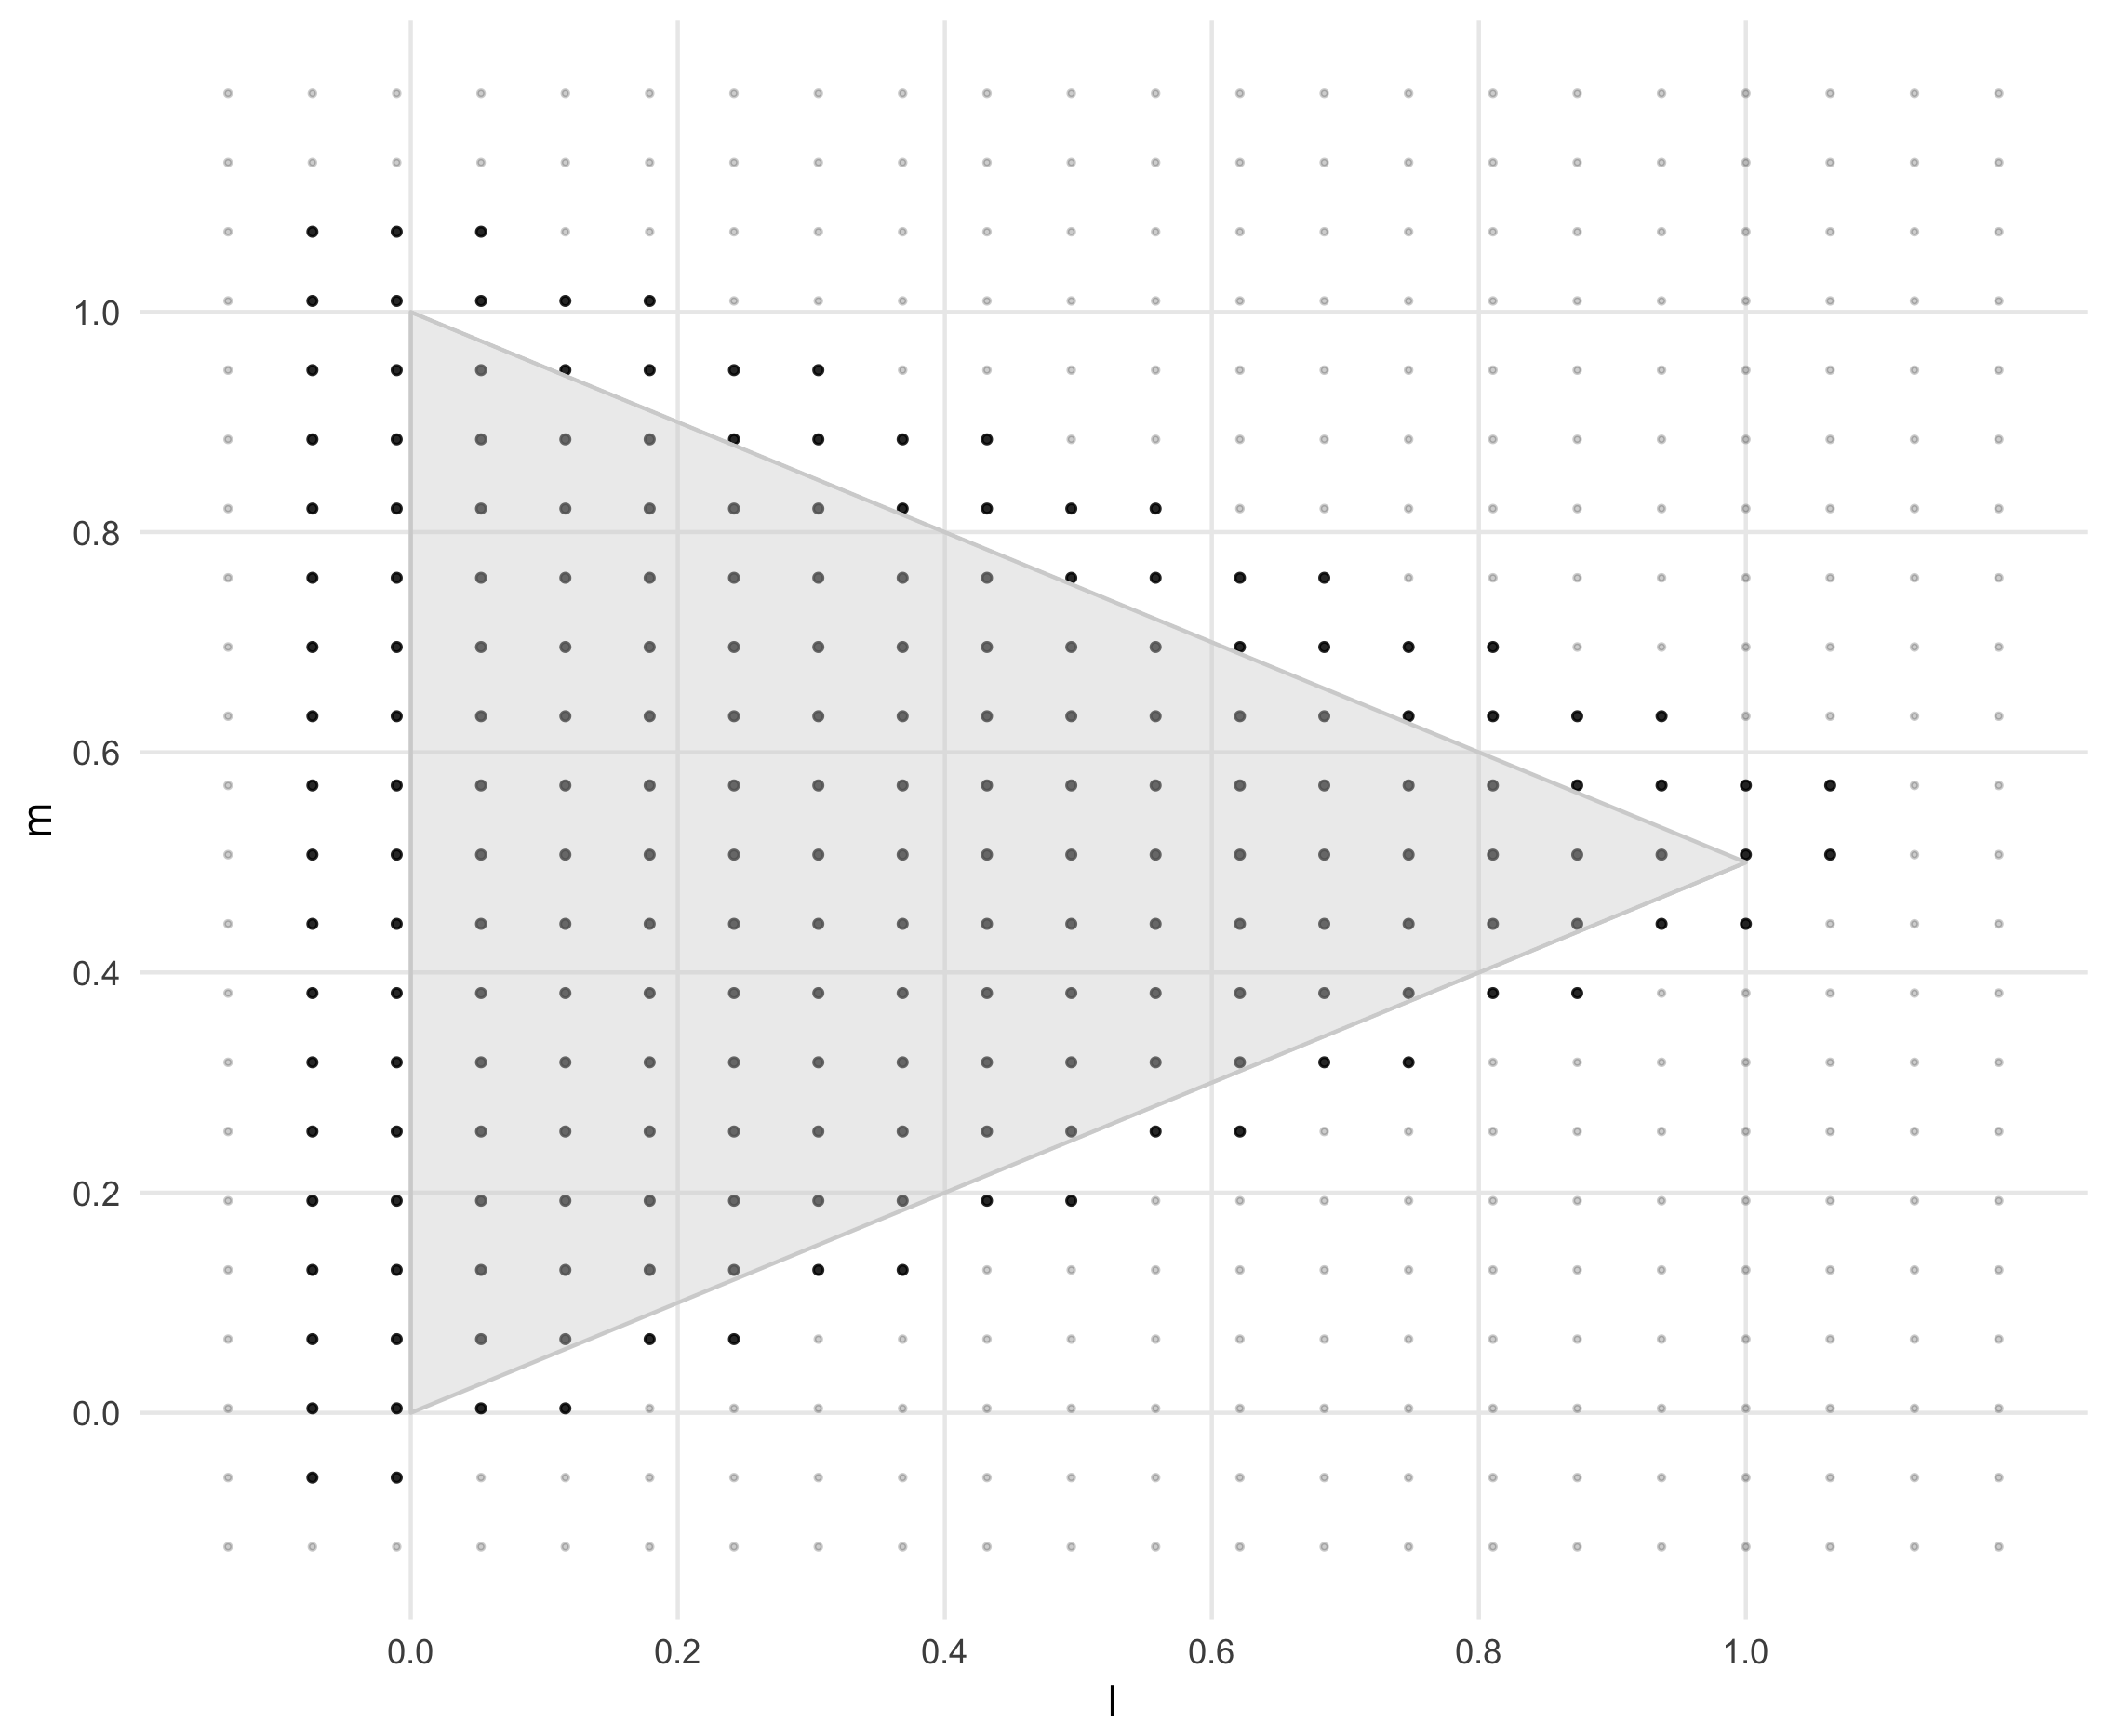
\includegraphics[scale=0.2]{knot-removal-on-triangle-domain.png}
 \caption{$\frac{l}{2} < m < 1 - \frac{l}{2}, \quad 0 < l < 1.$}
 \end{figure}

The triangular domain of $\phi^*$ cannot be modeled by the tensor product basis as constructed due to singularities resulting from the large number of basis functions anchored at knots near which we have no data, and hence little information about the corresponding basis coefficient. Much work in computer graphics has been done proposing methods of smoothing over arbitrary function domains, which are approximated by triangulations. See \citet{dahmen1992blossoming} and \citet{seidel1991symmetric} for details. These methods are, however, quite computationally intensive; to correct for the instability in the smoothed surface, we can simply remove the knots corresponding to tensor products functions which do not overlap with the function domain from the basis, $B$, and trimming the penalty matrices $P_l$ and $P_m$ as needed. With the trimmed basis and penalties, we can carry out optimization as previously discussed.



\section{Model selection and tuning parameter estimation}

\subsection{The limiting behaviour of $H_\lambda$}


The inspection of the hat matrix 

\[
H_\lambda = W B\left(W B^\prime W B +  \lambda_l P_l + \lambda_m P_m \right)^{-1} \left(W B\right)^\prime D^{-1}.
\]
\noindent
and its properties are integral for assessing model complexity and selecting the optimal values of the tuning parameters $\lambda_l$ and $\lambda_m.$  Summarizing the complexity of a fitted P-spline is far from a trivial task; one must simultaneously consider the value of the smoothing parameter, the number of basis functions in the B-spline basis, as well as the order of the difference penalties. We follow \citet{eilers1996flexible} and\citet{marx2005multidimensional} assess model complexity as discussed in cite{hastie1990generalized}, who proposed to use the trace of the smoother matrix as an approximation  to the effective dimensions of linear smoother. The \emph{effective dimension} is easily obtained and combines the effect of all three of these elements: 

%This approach to approximating the effective model dimension is also consistent with \citet{ye1998measuring}, who constructed a generalization of the concept of a model's degrees of freedom using the idea that the degrees of freedom can also be interpreted as the sum of the sensitivity of each fitted value with respect to the corresponding observed value.  For smoothing matrix $H$, the predicted response values are given by $\hat{y} = H y$. Writing
%
%\begin{align*}
%\frac{\partial \hat{y_i}}{\partial y_i} = \frac{\partial }{\partial y_i} \sum_{j} h_{ij} y_j = h_{ii},
%\end{align*}
%\noindent
%we see that the latter interpretation of the effective model dimension reduces to calculating the trace of the hat matrix. Thus we take the effective dimension to be 
%\begin{align}
%\textup{ED}\left(\lambda\right) &= \textup{tr}\left(H\right) \nonumber \\
%&= \textup{tr}\bigg[ B\left( B^T B + \lambda D^T D \right)^{-1} B^T\bigg], \label{eq:hat_matrix_trace}
%\end{align}

\begin{align}
\begin{split} \label{eq:hat-matrix-trace}
\textup{ED} &= \textup{tr} \left[ H_\lambda \right]\\
&= \textup{tr}\bigg[\left[WB \left(WB\right)^\prime D^{-1}WB +  \lambda_l P_l+ \lambda_m P_m\right]^{-1} \left(W B\right)^\prime D^{-1}  \bigg]
\end{split}
\end{align}
\noindent
When the number of basis functions is significantly smaller than the sample size, it is computationally advantageous to use the cyclic property of the trace: 

\begin{equation*}
\textup{tr}\bigg[\left[ \left(WB\right)^\prime D^{-1}WB +  \lambda_l P_l+ \lambda_m P_m\right]^{-1} \left(W B\right)^\prime D^{-1} WB  \bigg],
\end{equation*}
\noindent
which requires computing the trace of a $KL \times KL$ matrix. The effective dimension approaches $d_l + d_m$, the order of the differencing operator, as $\lambda$ increases, where $d_l$ and $d_m$ denote the orders of the difference penalties in the $l$ and $m$ directions, respectively.  Let
\begin{equation*}
Q = \left(W B\right)^\prime D^{-1} WB \qquad \mbox{and} \qquad Q_\lambda = P.
\end{equation*}
Using properties of the matrix trace, we can write
\begin{align*}
%\begin{split}
\mbox{tr}\left(H_\lambda \right) &= \mbox{tr}\bigg[ \left(Q + Q_\lambda \right)^{-1}Q \bigg]\\
&=\mbox{tr}\bigg[ Q^{1/2}\left(Q + Q_\lambda \right)^{-1}Q^{1/2} \bigg] \\
&=\mbox{tr}\bigg[\left(I + Q^{-{1/2}}Q_\lambda Q^{-{1/2}} \right)^{-1} \bigg]
%\end{split}
\end{align*}
Define $L \equiv Q^{-{1/2}}Q_\lambda Q^{-{1/2}}$. Then
\begin{equation*}
\mbox{tr}\left(H_\lambda \right) = \mbox{tr}\bigg[\left(I + \lambda L \right)^{-1} \bigg] = \sum_{j=1}^n \frac{1}{1 + \lambda \gamma_j}
\end{equation*}
 where $\gamma_j$, $j=1,\dots,n$ are the eigenvalues of $L$. $Q_\lambda$ has exactly $d_l + d_m$ eigenvalues equal to zero. Hence, $L$ has $d_l + d_m$ zero eigenvalues. For large $\lambda$, only the $d_l + d_m$ terms with $\gamma_j=0$ contribute to the sum which gives the trace of $H$, so that
 \[
\lim_{\lambda \rightarrow \infty  } \mbox{tr}\left(H\right) = d_l + d_m.
 \]
%
%A further simplification of \ref{eq:hat-matrix-trace}
%
%\begin{align*} 
%\left(B^T B + \lambda D^T D \right)^{-1} B^T B &= \left(B^T B + \lambda D^T D \right)^{-1} \left( B^T B + \lambda D^T D - \lambda D^T D\right) \nonumber \\
%&= I - \lambda\left(B^T B + \lambda D^T D \right)^{-1} D^T D \label{eq:cyclic_hat_matrix_simplification}
%\end{align*}
%
%\begin{align*} 
%\left[\left(WB\right)^\prime D^{-1}WB +  \lambda_l P_l+ \lambda_m P_m\right]^{-1} \left(W B \right)^\prime D^{-1} WB  &= \left[\left(WB\right)^\prime D^{-1}WB +  \lambda_l P_l+ \lambda_m P_m\right]^{-1}\left(W B \right)^\prime D^{-1} \times \\
%&\mbox{\;\;\;\;\;\;\;\;\;\;\;\;\;\;\;\;\;\;\;\;\;} \left[WB + \lambda_l P_l+ \lambda_m P_m - \left(\lambda_l P_l+ \lambda_m P_m\right) \right] \\
%&= I - \lambda\left(B^T B + \lambda D^T D \right)^{-1} D^T D \label{eq:cyclic_hat_matrix_simplification}
%\end{align*}
%
%
%
%Equation~\ref{eq:cyclic_hat_matrix_simplification} cleanly shows that the effective dimension is always less than $n$, the number of B-spline used in the regression basis; further, the effective dimension is always smaller than $\min\left(m,n\right)$. A formal proof follows below. This is illustrated in 
%
%Figure~\ref{fig:PS_ED_figure_1} shows how the effective dimension on a univariate P-spline changes with the smoothing parameter for the ten simulated observations in Figure~\ref{fig:overcomplete_basis_pspline} using 60 B-spline basis functions. For small $\lambda$, the effective dimension approaches $m$. As $\lambda$ increases, the effective dimension approaches the order of the difference penalty, $d$. It is worth pointing out here that there are no problems incurred when smoothing with many more B-splines than observations since the effective model dimension is always less than $m$, for all $\lambda$. 
%
%
%\begin{figure}[H]
%\begin{subfigure}{.5\textwidth}
%  \centering
%   \graphicspath{{img/}}
%  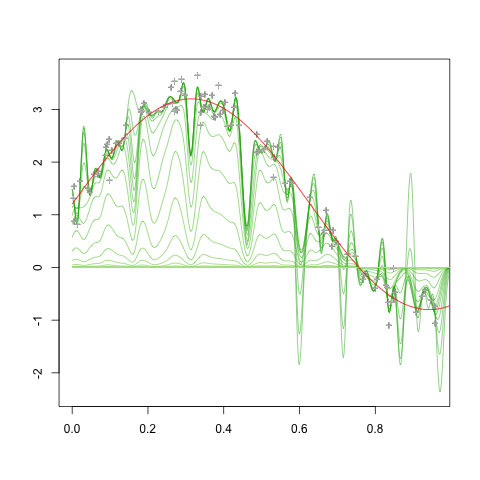
\includegraphics[scale=0.5]{PS_penalty_section_figure_6_order_0.png}
%  %\label{fig:pspline_small_lambda}
%\caption{$d=0$ }
%\end{subfigure}
%\begin{subfigure}{.5\textwidth}
%  \centering
%   \graphicspath{{img/}}
%  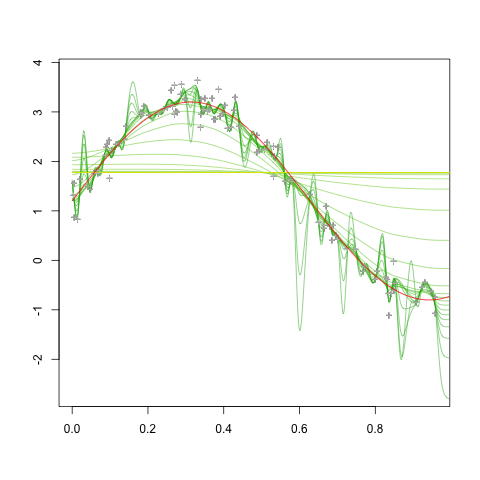
\includegraphics[scale=0.5]{PS_penalty_section_figure_6_order_1.png}
% % \label{fig:pspline_small_lambda}
%\caption{$d=1$}
%\end{subfigure}
%\begin{subfigure}{.5\textwidth}
%  \centering
%   \graphicspath{{img/}}
%  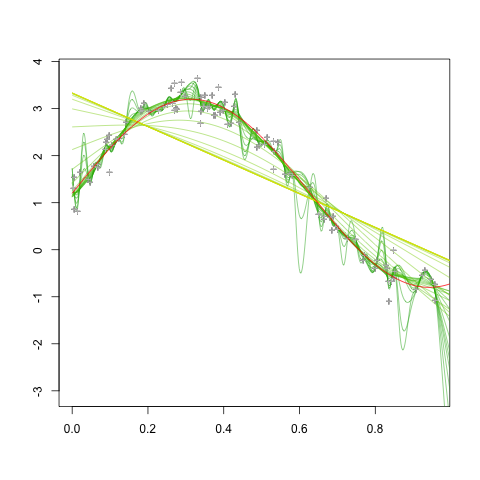
\includegraphics[scale=0.5]{PS_penalty_section_figure_6_order_2.png}
%  %\label{fig:pspline_small_lambda}
%\caption{$d=2$}
%\end{subfigure}
%\begin{subfigure}{.5\textwidth}
%  \centering
%   \graphicspath{{img/}}
%  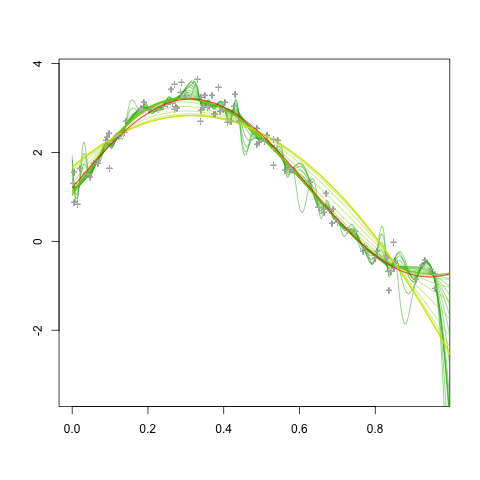
\includegraphics[scale=0.5]{PS_penalty_section_figure_6_order_3.png}
%  %\label{fig:pspline_small_lambda}
%\caption{$d=3$}
%\end{subfigure}
%\caption{\textit{Illustration of the impact of the order of the difference penalty. The number of B-splines used is the same in each plot, with the penalty parameter varying from across the same grid of values. The fitted curves in the upper left plot correspond to the difference penalty of order $0$, where $\vert D_0 \alpha \vert^2 = \sum_{i=1}^n \alpha_i^2$, analogous to ridge regression using the B-spline basis as regression covariates. The fitted curves approach polynomials of degree $d-1$ as $\lambda \rightarrow \infty$, as discussed in \ref{eq:PS_properties} \ref{eq:PS_property_3}.}}
%\label{fig:PS_penalty_section_figure_6}
%\end{figure}
%



\end{document}
 
%==============================================================================================================================================
%==============================================================================================================================================

\chapter{Modeling the Cholesky decomposition via penalized B-splines} \label{chapter-3}

\subsection{A B-spline representation for pp functions}

%\subfile{chapter-3-subfiles/chapter-3-bspline-representation}

\begin{definition} \label{definition:order_k_Bspline}
Let $t= \left\{ t_i \right\}$ denote a non-decreasing sequence. The $i^{th}$ B-spline of order $k$ which corresponds to the knot sequence $t$ is defined by 
\begin{equation} \label{eq:bspline_definition}
B_{i,k,t}\left(x\right) = \left(t_{i+k}-t_i\right)\left[t_i,\dots,t_{i+k}\right]\left(\cdot -x\right)_+^{k-1}
\end{equation}
\end{definition}

The placeholder notation, $\left(\cdot - x\right)_+^{k-1}$, is used to indicate that the $k^{th}$ divided difference of the function $g\left(t \right) = \left(t-x\right)^{k-1}_+$ is obtained by fixing $x$ and applying the divided difference to $g\left(t \right)$ as a function of $t$ alone. Henceforth, we will write $B_i$ rather than $B_{i,k,t}$ when the spline order and knot sequence can be inferred from surrounding context.

\subsection{Properties of B-splines}

\begin{enumerate} \label{eq:BS_properties}
\item \label{eq:BS_property_1} $B_i\left(x\right)$ has isolated support:
\[
B_i\left(x\right) = 0, \quad x \not \in \left[t_{i},t_{i+k}\right]
\]
To see this, note that if $x \not \in \left[t_{i},t_{i+k}\right]$, then $g\left(t \right) = \left(t-x\right)^{k-1}_+$ is a polynomial of degree $< k$ on $\left[t_{i},t_{i+k}\right]$, thus by \ref{dd_properties} \ref{eq:dd_property_5},
\[
\left[t_{i},\dots,t_{i+k}\right]g = 0.
\]
As a result, for a set of B-splines of order $k$ corresponding to the knot sequence $t$, only $k$ of them are nonzero on $\left[t_{j},t_{j+k}\right]$: $B_{j-k+1},B_{j-k+2},\dots,B_{j}$.
\item \label{eq:BS_property_2} The $i^{th}$ B-spline of order is defined as the $k^{th}$ divided difference of $\left(\cdot - x\right)_+^{k-1}$ times a normalization factor: $\left(t_{i+k}-t_i\right)$. This normalization, using \ref{dd_properties} \ref{eq:dd_property_8}, allows us to write 
\begin{equation} \label{eq:BS_norm_rr}
B_i\left(x\right)=\left[t_{i+1},\dots,t_{i+k} \right]\left(\cdot - x\right)_+^{k-1} - \left[t_{i},\dots,t_{i+k-1} \right]\left(\cdot - x\right)_+^{k-1}
\end{equation}
For $x \in \left(t_{j},t_{j+1}\right)$, by \ref{dd_properties} \ref{eq:dd_property_1},
\begin{align}
\sum_{i} B_i\left(x\right) &=  \sum_{i=j+1-k}^{j} B_i\left(x\right) \nonumber\\
&= \sum_{i=j+1-k}^{j} \left[t_{i+1},\dots,t_{i+k} \right] \left(\cdot - x\right)_+^{k-1} - \sum_{i=j+1-k}^{j} \left[t_{i},\dots,t_{i+k-1} \right] \left(\cdot - x\right)_+^{k-1} \nonumber \\
&= \left[t_{j+1},\dots,t_{j+k} \right] \left(\cdot - x\right)_+^{k-1} - \left[t_{j+1-k},\dots,t_{j} \right] \left(\cdot - x\right)_+^{k-1} \nonumber \\
&= 1 - 0 \label{eq:unity_equality}
\end{align}
The last equality in \ref{eq:unity_equality} is a consequence of the following: for $x \in \left(t_j,t_{j+1}\right)$, $g\left(t\right)=\left(t - x\right)_+^{k-1}$ is a $k-1$ degree polynomial with unit leading coefficient on $\left[ t_{j+1},t_{j+k} \right]$, so by \ref{dd_properties} \ref{eq:dd_property_5}, 
\[
\left[ t_{j+1},\dots,t_{j+k} \right]g=1.
\]
On $\left[ t_{j+1-k},t_{j} \right]$, $g$ is identically $0$, hence $\left[ t_{j+1-k},\dots,t_{j} \right]g = 0$.   
\item \label{eq:BS_property_3}Each $B_i\left(x\right)$ is positive on its support. Applying Leibnitz's formula (\ref{dd_properties} \ref{eq:dd_property_4}) to the product
\[
\left[t_i,\dots,t_{i+k} \right]\left(t-x\right)_+^{k-1} = \left[t_i,\dots,t_{i+k} \right]\left(t-x\right) \left(t-x\right)_+^{k-2},
\] 
we have
\begin{align}
\left[t_i,\dots,t_{i+k} \right]\left(t-x\right)_+^{k-1} &=  \left[t_i,\dots,t_{i+k} \right]\left(t-x\right) \left(t-x\right)_+^{k-2} \nonumber\\
&= \sum_{r=i}^{i+k}\left[t_i,\dots,t_{i+r} \right] \left(t-x\right)\left[ t_r,\dots,t_{i+k}\right]\left(t-x\right)_+^{k-2} \nonumber \\
&= \bigg[ \left[t_i\right]\left(t-x \right) \bigg]\bigg[ \left[ t_i,\dots,t_{i+k}\right]\left(t-x\right)_+^{k-2}\ \bigg]\nonumber \\
& \qquad \qquad + \bigg[ \left[t_i,t_{i+1}\right]\left(t-x \right) \bigg]\bigg[ \left[ t_{i+1},\dots,t_{i+k}\right]\left(t-x\right)_+^{k-2} \bigg] \nonumber \\
&= \left(t_i-x \right) \left[ t_{i},\dots,t_{i+k}\right]\left(t-x\right)_+^{k-2} \nonumber \\
& \qquad \qquad \qquad \qquad \qquad +  1 \cdot \left[ t_{i+1},\dots,t_{i+k}\right]\left(t-x\right)_+^{k-2} \label{eq:nonneg_star}
\end{align}
since $\left[ t_i,\dots,t_j\right]\left(\cdot-x\right) = 0$ for $j>i+1$. By \ref{dd_properties} \ref{eq:dd_property_8}, 
\[
\left(t_i-x \right) \left[ t_{i},\dots,t_{i+k}\right]g = \frac{t_i-x}{t_{i+k}-t_{i}}\bigg[\left[ t_{i+1},\dots,t_{i+k}\right]g -\left[ t_{i},\dots,t_{i+k-1}\right]g   \bigg],
\]
and we may express \ref{eq:nonneg_star} as 
\begin{align*}
\left[ t_{i},\dots,t_{i+k}\right]\left(\cdot - x\right)^{k-1}_+ &= \frac{x-t_i}{t_{i+k}-t_{i}}\left[ t_{i},\dots,t_{i+k-1}\right] \left(\cdot-x\right)_+^{k-2}  \\
& \quad + \frac{t_{i+k}-x}{t_{i+k}-t_{i}}\left[ t_{i+1},\dots,t_{i+k}\right] \left(\cdot-x\right)_+^{k-2} 
\end{align*}
which we can write in terms of the normalized B-spline:
\begin{equation} \label{eq:nonneg_starstar}
\frac{B_{i,k}\left(x\right)}{t_{i+k}-t_i} = \frac{x-t_i}{t_{i+k}-t_{i}}\frac{B_{i,k-1}\left(x\right)}{t_{i+k-1}-t_i} + \frac{t_{i+k}-x}{t_{i+k}-t_{i}} \frac{B_{i+1,k-1}\left(x\right)}{t_{i+k}-t_{i+1}}
\end{equation}
This shows that we can write the $i^{th}$ B-spline of order $k$ as a convex combination of the $i^{th}$ and $\left(i+1\right)^{st}$ B-splines of order $k-1$ since 
\[
\frac{x-t_i}{t_{i+k}-t_{i}} + \frac{t_{i+k}-x}{t_{i+k}-t_{i}}  = 1,
\]
and each of these weights are positive for $t_i < x < t_{i+1}$. If
\[
\begin{array}{lr}
B_{j,k-1}\left(x\right) > 0, & t_j < x < t_{j+k-1} \; \textup{for all } j,
\end{array}
\]
then by \ref{eq:nonneg_starstar}, we have that 
\[
B_{i,k}\left(x\right) > 0,  \qquad t_i < x < t_{i+k}
\]
since $B_{j,k-1}= 0$ for $x \not \in \left[t_j,t_{j+k}\right]$ by \ref{eq:BS_properties} \ref{eq:BS_property_1} and by induction over $k$, starting with the fact that 
\[
B_j,1\left(x\right) = \left\{ \begin{array}{lr}
1 & t_j \le x < t_{j+1}\\
0 & otherwise
\end{array}\right.
\]
Properties \ref{eq:BS_property_1}, \ref{eq:BS_property_2}, and \ref{eq:BS_property_3} demonstrate that a sequence of B-splines form a \emph{partition of unity}: a set of non-negative functions which sum, pointwise, to one.
\end{enumerate}

%\begin{example}
%Figure~\ref{fig:deboor_bspline_basis} show fives parabolic B-splines corresponding to the set of knots $\left\{0,1,1,3,4,6,6,6 \right\}$. It is clear that each spline has compact support and is non-negative on this support. The function values are provided at select domain values so that property \ref{eq:BS_property_2} is evident, though it is worth noting that 
%\[
%\sum_{i=1}^6 B_i\left(x\right) = 1
%\]
%only on $\left[\frac{1}{6},1\right]$. In particular, they do not sum to 1 on $\left(0,\frac{1}{6}\right)$. 
%
%Each $B_i$ is piecewise parabolic, with the breakpoints being locations of discontinuity of the function or one of its derivatives. $B_5$ is discontinuous at $x=6$, as the knot at 6 is repeated three times in the knot sequence defining $B_5$: $\left\{t_5,t_6,t_7,t_8\right\}$.
%
%$B_1$, $B_2$, and $B_4$ have discontinuous first derivatives since 1 is repeated twice in the knots defining $B_1$ and $B_2$, and 6 is repeated twice in the knots defining $B_4$. The relationship between knot replication and smoothness will be discussed in more detail in the following section.
%
%\begin{figure}[h]
% \begin{center}
% \graphicspath{{img/}}
%  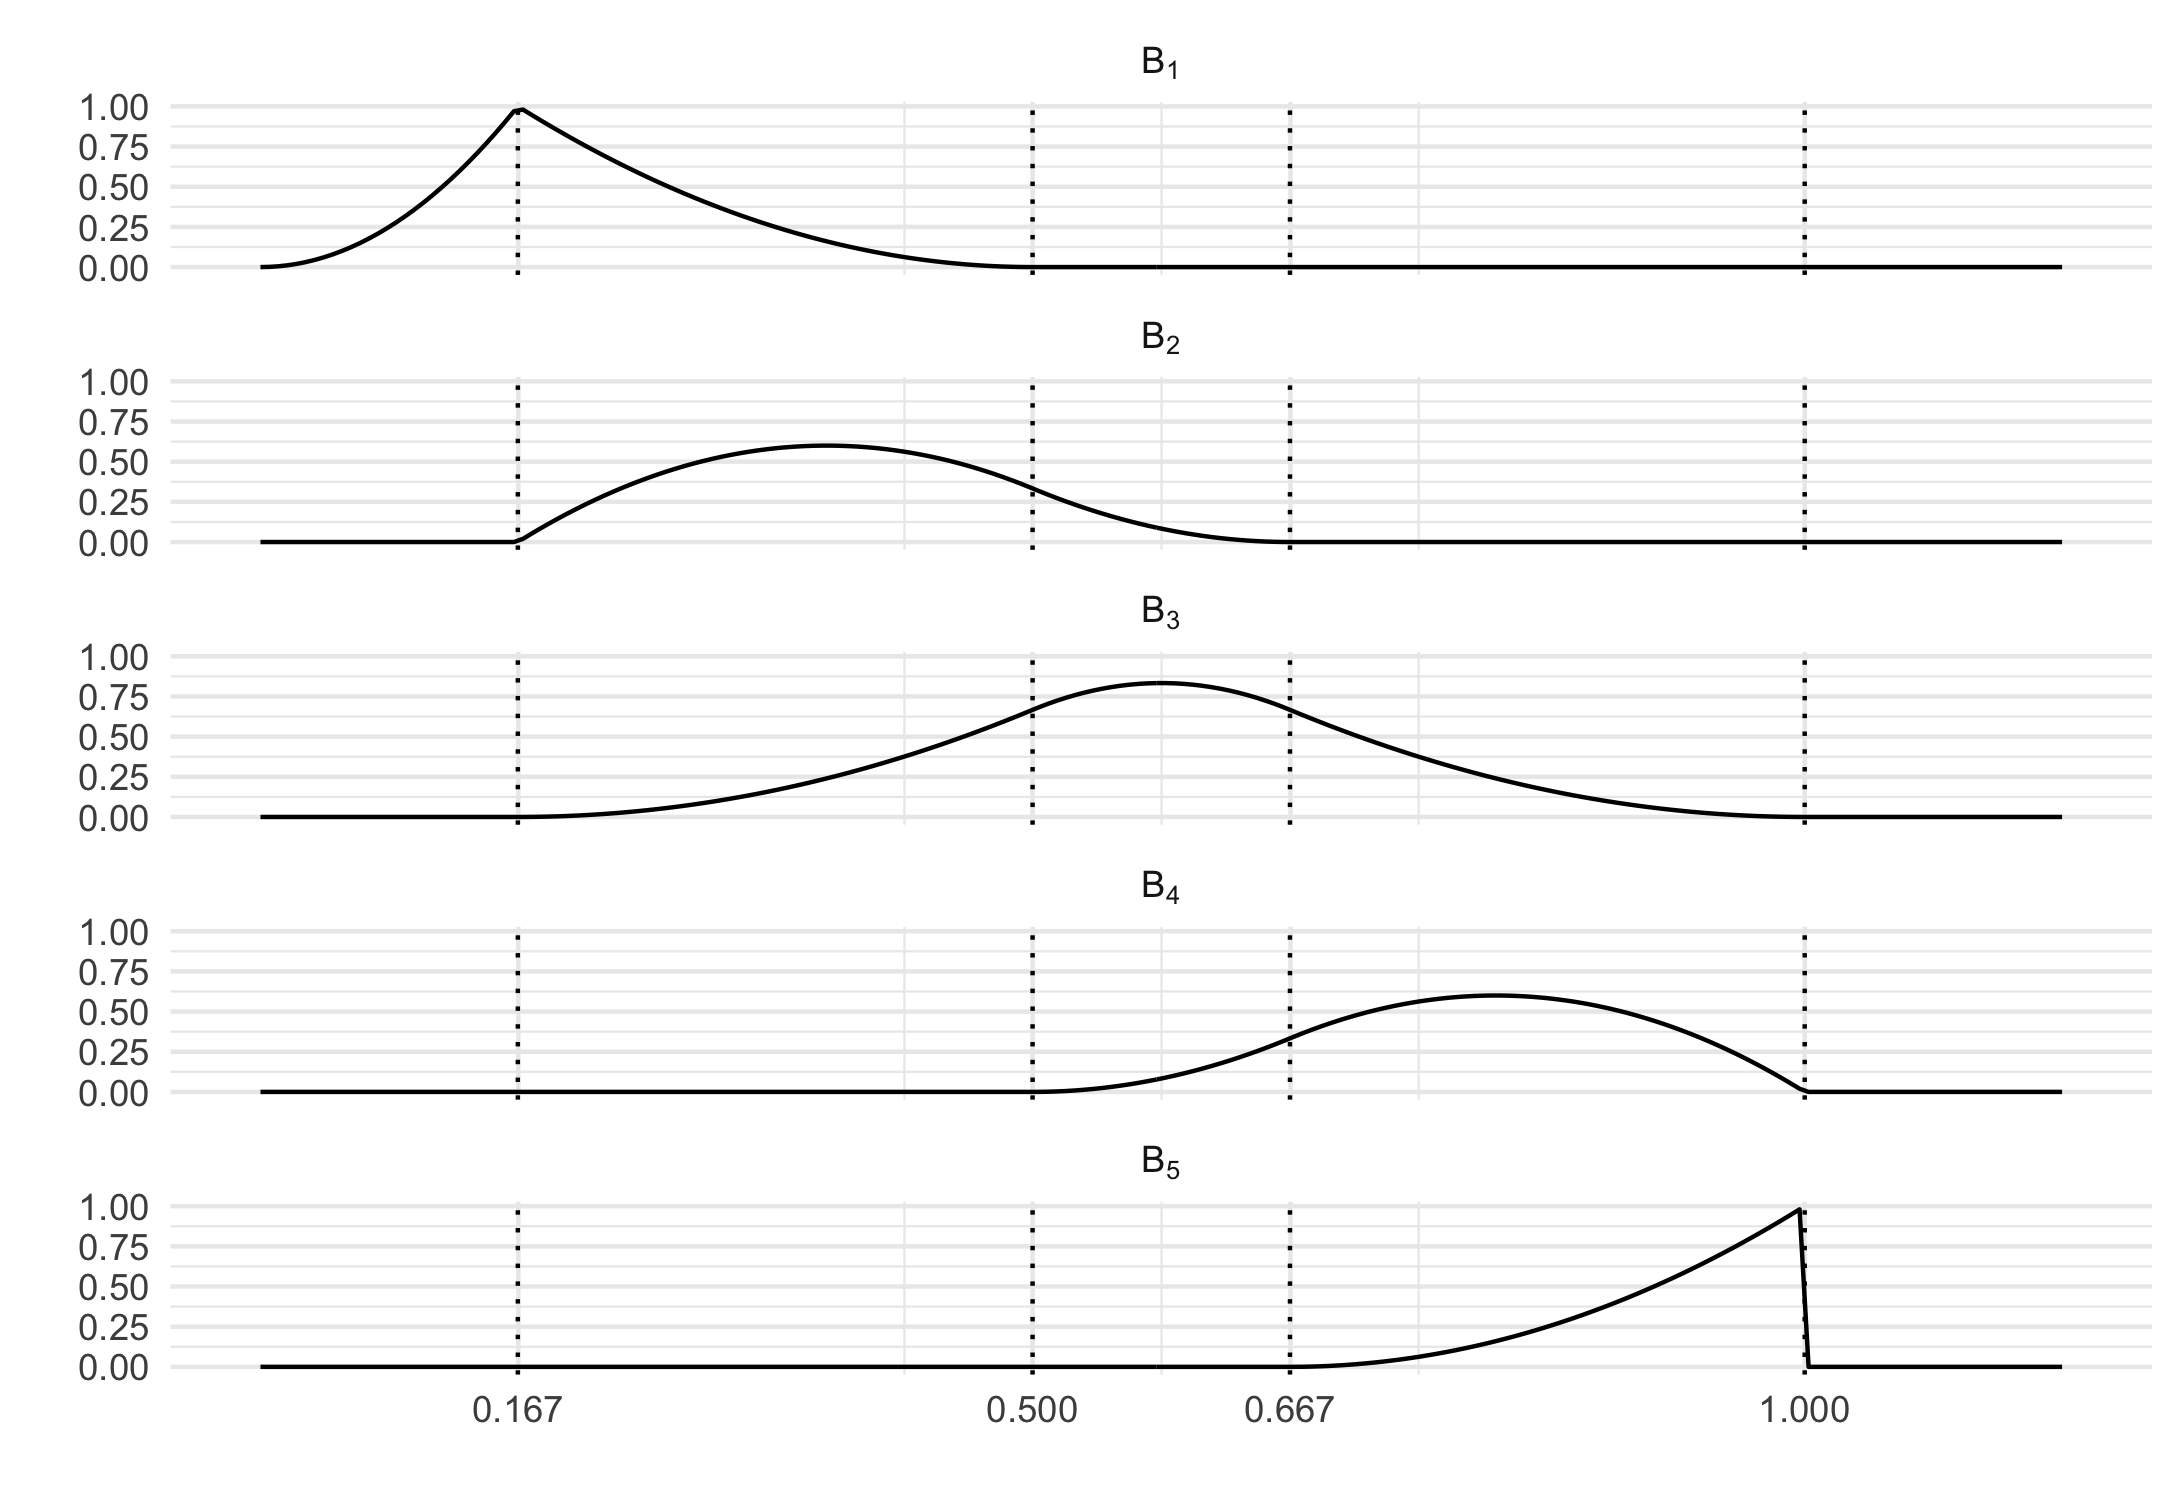
\includegraphics{deboor_parabolic_bsplines.png}
%  %\caption{Parabolic B-splines corresponding to knot sequence $\{0,1,1,3,4,6,6,6\}$, illustrating the connection between knot multiplicity and smoothness.}\label{fig:deboor_bspline_basis}
%\end{center}
%\end{figure}
%\end{example}

\begin{definition} \label{B_representation_definition}
The \emph{B-representation of } $f \in \PP_{k,\xi,\nu}$ consists of 
\begin{enumerate}
\item \label{eq:first_B_rep_piece} integers $k$ and $n$ specifying the order of $f$ as a pp function and the number of linear parameters, 
\[
n = kl - \sum_{i}\nu_i = \mbox{dim}\left(\PP_{k,\xi,\nu}\right),
\]
respectively. 
\item \label{eq:second_B_rep_piece}The knot vector $t = \left \{t_i \right\}$, $i=1,\dots, n+k$ with elements arranged in increasing order, constructed according to Theorem~\ref{curryschoenbergthm}, via $\xi$ and $\nu$.
\item \label{eq:third_B_rep_piece} The B-spline coefficients $\alpha=\left \{\alpha_i \right\}$, $i=1 ,\dots, n$ for the knot sequence, $t$.
\end{enumerate}
\end{definition}
\vspace{1pt}
Given \ref{eq:first_B_rep_piece}, \ref{eq:second_B_rep_piece}, and \ref{eq:third_B_rep_piece} in \ref{B_representation_definition}, the function value at $x\in \left[t_k, t_{n+1}\right]$ is given by 
\begin{equation*}
f\left(x\right) = \sum_{i=1}^n \alpha_i B_i\left(x\right),
\end{equation*}
and in particular, by \ref{eq:BS_property_1}, for $x\in \left[t_j, t_{j+1} \right]$,
\[
f\left(x\right) = \sum_{i=j}^{j+k-1} \alpha_i B_i\left(x\right).
\]

%%==============================================================================================================================================
%%==============================================================================================================================================
%%==============================================================================================================================================
%%==============================================================================================================================================
%%==============================================================================================================================================
%%==============================================================================================================================================
%%==============================================================================================================================================
\subsection{Single-regressor varying coefficient models via B-spline basis expansions}

\cite{hastie1993varying} were the first to introduce the varying coefficient model, which supplies a modeling approach which permits interpolation of regressors and response variables which varying according to an \emph{indexing variable} at values of this indexing variable where there is either missing data of only a single observation and slope estimation is not feasible. In the section that follows, we will discuss the approach to smoothing the coefficient vector (and \emph{not} the regressor, $x\left(t\right)$) first, for mechanical demonstration of parameterization and estimation of the coefficient function via B-spline basis expansion, at a predetermined set of values of an indexing variable, $t$ (knots), then following the approach of Eilers and Marx by assuming that the number and position of the knots are unknown and using penalized B-splines, or P-splines. 

\bigskip

Consider data of the form 
\[
\left(x_i, y_i, t_i\right), \qquad i=1,\dots,m
\]
where $y_i$ is the response, $x_i$ is the single (univariate) regressor variable, and $t_i$ is an indexing variable. We first consider a simple situation as an introductory warmup for demonstrating the mechanics of the varying coefficient model. Suppose we wish to fit a scatterplot smoother to the points $\left(t_i, y_i\right)$ using a B-spline basis expansion. Assume that we can model 

\begin{equation} \label{eq:varying_intercept_only_model}
y\left(t\right) = f\left(t\right) + \epsilon\left(t \right)
\end{equation}
\noindent
where $\epsilon$ is a zero-mean error process.  Modeling the mean function as a $q^{th}$-order B-spline, we can rewrite \ref{eq:varying_intercept_only_model} as

\begin{equation} \label{eq:varying_intercept_only_model_bspline}
y\left(t\right) = \sum_{j=1}^{K} \alpha_j B_j\left(t\right) + \epsilon\left(t \right)
\end{equation}
\noindent
Assume we use $K$ of basis functions in our expansion of $f$. Let $y= \left(y_1,\dots,y_M\right)^T$, and let $B$ denote the $M \times K$ design matrix with $i-j^{th}$ element given by the $j^{th}$ order-$q$ B-spline evaluated at the $i^{th}$ value of $t$: 

\[
b_{ij} = B_j\left(t_i\right),
\]
$i=1,\dots,m$, $j=1,\dots,K$. Then in matrix notation, we may write the mean vector

\[
\mu = E\left[Y\right] = B\alpha
\]
\noindent
where $\alpha$ is the vector of $K$ unknown basis coefficients. We take $\hat{\alpha}$ to be the minimizer of 

\begin{align}
S &= \sum_{i=1}^M \left(y_i - \sum_{j=1}^{K} \alpha_j B_j\left(t_i\right) \right)^2 \nonumber\\
&=\vert y - B\alpha \vert^2 \label{eq:S_varying_intercept_model}
\end{align}


\[
B^TB\alpha = B^Ty
\]
which has explicit solution
\[
\hat{\alpha} = \left(B^T B\right)^{-1}B^Ty
\]
\noindent
Given $\hat{\alpha}$, one may estimate the response at any new value of $t$, say $t^*$, by 
\[
\hat{y}\left(t^*\right) = \sum_{j=1}^{K} \hat{\alpha_j}B_j\left(t^*\right).
\]

\subsection{B-spline estimators for varying coefficient models with fixed knots}

To extend the varying intercept model \ref{eq:varying_intercept_only_model} to accommodate for controlling for another regressor, it is natural to consider the varying coefficient model; the single regressor varying-coefficient (VC) model extends the classical linear model by allowing the slope coefficient to vary smoothly in the dimension of the indexing variable, $t$.  The single-index varying coefficient model assumes that the mean response is of the form

\begin{equation} \label{eq:simplest_VC_model_mean}
E\left[ Y\left(t\right) \right] = \beta_0\left(t\right) + \beta_1\left(t\right)x\left(t\right)
\end{equation}

where $\beta_0\left(t\right)$ is the smooth varying intercept function and $\beta_1\left(t\right)$ is the smooth slope function of interest. This model generalizes the well known simple linear regression model 
\[
E\left[Y\left(t\right)\right] = \beta_0 + \beta_1 x\left(t\right)
\]
by trading the static regression coefficients for smooth coefficient functions which are assumed to varying across an indexing variable, $t$. This allows for the regressor variable to having modified effect, depending on the value of $t$. Using a set of predetermined knots along the $t$ axis, the VC model can be fit in a fashion similar to that required for fitting model \ref{eq:varying_intercept_only_model}, requiring only minor adjustments to the design matrix. In matrix notation as described in \ref{eq:S_varying_intercept_model}, the mean vector may be written

\begin{equation} \label{eq:VC_mean_matrix}
\mu = B\alpha_0 + diag\left\{x\left(t\right) \right\}B\alpha_1
\end{equation} 
\noindent
where $diag\left\{x\left(t\right) \right\}$ is the $m \times m$ diagonal matrix of regressor measurements which ensures that the varying coefficients are appropriately weighted according to the correct value of $x$ by aligning the regressor function with the corresponding slope value. Letting $X = diag\left\{x\left(t\right) \right\}B$, \ref{eq:VC_mean_matrix} becomes

\begin{align}
\mu &= \left[ B | X \right] \left(\alpha_0^T,\alpha_1^T\right)^T \\
&\equiv Q\alpha
\end{align} 

where $\alpha$ is the augmented vector of basis coefficients. Here, the same basis is used for smoothing both the varying intercept as well as the varying slope function; this is feasible because both components varying along the same indexing variable. One can relax this structure and allow each additive term to varying according to its own indexing variable. This, of course, requires a separate B-spline basis for each component. Again using least squares techniques as with the varying intercept-only model, we take $\hat{\alpha}$ to minimize

\begin{equation} \label{eq:S_varying_intercept_slope_model}
S = \vert y-Q\alpha \vert ^2
\end{equation}
which has explicit solution

\[
\hat{\alpha} =\left(Q^T Q\right)^{-1} Q^Ty.
\]

It is worth noting that $Q$ is simply a row scaling of the original B-spline design matrix, $B$; thus, accommodating a varying slope function equates to the simple basis function regression setting with a modified basis, $XB$. Using the modified basis functions as covariates, estimation of model the varying coefficient model equates to a multiple regression problem. Each of the estimated smooth components are given by 
\[
\hat{\beta}_k\left(t \right)= B\hat{\alpha}_k, \qquad k=0,1
\]
\noindent
and the estimate of the smooth mean function is obtained via 
\begin{align*}
\hat{\mu} &= Q\hat{\alpha}\\
&= Hy
\end{align*}
where $H = Q\left(Q^T Q\right)^{-1} Q^T$ is the ``hat'' matrix, which is analogous to the smoothing matrix $\tilde{A}$ referred to in the discussion of the smoothing spline estimation of $\phi$ in Chapter 2. Its use in smoothing parameter selection and model tuning is similar to the reproducing kernel Hilbert space framework, which we will discuss in the coming sections.


%\subfile{chapter-3-subfiles/chapter-3-bspline-single-index-vc-models}
%%==============================================================================================================================================
%%==============================================================================================================================================
%%==============================================================================================================================================
%%==============================================================================================================================================
%%==============================================================================================================================================
%%==============================================================================================================================================

\subsection{P-spline estimators for regularized estimation of fitted curves}

The mechanics in the previous section rely on apriori knowledge of the number and locations of the knots $\left\{t_j\right\}$, $j=1,\dots,K$. In practice this information is readily available, but has a considerable impact on the behaviour of the estimated coefficient functions, as the smoothness of a fitted curve can be controlled by the number of B-splines used in the basis expansion used to approximate the curve. Fewer knots (thus, fewer basis functions) lead to smoother fits. This choice presents a model selection problem, as too many knots lead to overfitting while too few knots lead to underfitting. Optimal knot placement has been closely examined, with some authors proposing automatic methods for optimizing the number and the positions of the knots (\cite{friedman1989flexible}, \cite{stone1997polynomial}). This is a difficult numerical problem requiring nonlinear optimization, and is still an open problem today. However, limiting the number of B-splines is not the only approach to controlling the complexity of the fitted function. 

\bigskip

As in Chapter 2, we can append a penalty on the coefficients of the basis functions to the goodness of fit measure, and by optimizing this augmented objective function, we can achieve as much smoothness in the fitted function as desired. \cite{o1986statistical} was the first to propose using a rich B-spline basis and applying a discrete penalty to the spline coefficients.  He proposed a penalty on the second derivative to restrict the flexibility of the fitted curve, similar to the penalty pioneered for smoothing splines by \cite{reinsch1967smoothing}. This penalty has become the standard in much of the spline literature; see \cite{eubank1999nonparametric}, \cite{wahba1990spline}. This measure of roughness of a curve is given by 
 
 \[
 J = \int_l^u \left[ f^{\prime \prime}\left(x\right)\right]^2\;dx
 \]
 \noindent
 where $l$ and $u$ are the bounds on the domain of $x$. Using the properties of B-splines, if $f\left(x\right) = \sum_{j} \beta_j B_j\left(x\right)$, one can derive a banded matrix $P$ such that 
 \[
 J = \beta^\prime P \beta
 \] 
 \noindent
 where $\beta = \left(\beta_1,\dots, \beta_n\right)$, and the $i$-$j^{th}$ element of $P$ is given by
 \[
 p_{ij} = \int_l^u B_i^{\prime \prime} \left( x \right)B_j^{\prime \prime} \left( x \right)\;dx.
 \]
 \noindent
 He then proposed minimizing
 \begin{eqnarray*}
 Q\left(\beta, \lambda \right) &=& \sum_{i=1}^m \left(y_i - \sum_{j} \beta_j B_j\left(x_i \right)\right)^2 + \lambda \int_l^u \left[ f^{\prime \prime}\left(x\right)\right]^2\;dx\\
 &=& \vert y - B\beta \vert  \vert^2 + \lambda\beta^\prime P \beta
 \end{eqnarray*}

The computation of $P$ is nontrivial and becomes very tedious when the third and fourth derivative are used as the roughness measure. \cite{wand2008semiparametric} extend O'Sullivan's work to higher order derivatives for general degree B-splines and derive an exact matrix algebraic expression for the penalty matrices. In the cubic case, the expression is a result of the application of Simpson's Rule applied to the inter-knot differences since each $B_i^{\prime \prime} B_j^{\prime \prime}$ is a piecewise quadratic function. The penalty may be written
 \[
 P = \left(B^{\prime \prime}\right)^\prime \textup{diag}\left(\omega \right) B^{\prime \prime}, 
 \]
 \noindent
 where $B^{\prime \prime}$ is the $3\left( n + 7 \right) \times \left( n + 4 \right)$ matrix with $i$-$j^{th}$ entry given by $B_j^{\prime \prime} \left(x_i^*\right)$, $x^*_i$ is the $i^{th}$ element of 
 
\[
\left( \phi_1,\frac{\phi_1+\phi_2}{2},\phi_2,\phi_2,\frac{\phi_2+\phi_3}{2},\phi_3,\dots,\phi_{n+7},\frac{\phi_{n+7}+\phi_{n+8}}{2},\phi_{n+8} \right),
\]
 \noindent
 and $\omega$ is the $3\left(n+7\right) \times 1$ vector given by
 
\begin{align*}
\omega &= \left( \frac{1}{6}\left(\Delta \phi \right)_1,\frac{4}{6}\left(\Delta \phi \right)_1, \frac{1}{6}\left(\Delta \phi \right)_1,\frac{1}{6}\left(\Delta \phi \right)_2, \frac{4}{6}\left(\Delta \phi \right)_2,  \right. \\
&\qquad   \left. {} \frac{1}{6}\left(\Delta \phi \right)_2 , \dots , \frac{1}{6}\left(\Delta \phi \right)_{n+7}, \frac{4}{6}\left(\Delta \phi \right)_{n+7}, \frac{1}{6}\left(\Delta \phi \right)_{n+7}  \right) \\
\end{align*}
\noindent
 where $\left(\Delta \phi \right)_j = \phi_{j+1}-\phi_j$. They generalize this to the case of any order penalty and present a table of formulas for constructing any arbitrary penalty matrix, $P$.
 
%\subfile{chapter-3-subfiles/chapter-3-pspline-models-intro}
%%==============================================================================================================================================
%%==============================================================================================================================================
%%==============================================================================================================================================
%%==============================================================================================================================================
%%==============================================================================================================================================
%%============================================================================================================================================== 
\subsubsection{Difference penalties}

Imposing difference penalties on B-spline basis expansions generalizes and simplifies the approach outlined in the previous section in a way that permits application in any context where regression on B-splines is useful. Penalized B-splines, or \emph{P-splines}, are an alternative an approach to nonparametric smoothing which circumvent any complexity associated with constructing such penalty matrices by ommitting derivatives and integrals altogether. Instead, smoothness is imposed via a discrete penalty matrix based on finite difference formulas which is simple to compute. This approach achieves smoothness in fitted functions in two ways:

\begin{enumerate}
\item To avoid the difficulty of choosing the optimal set of knots, use a B-spline basis with a large number of equally spaced knots, purposefully overfitting the smooth coefficient vectors. 
\item Augment the goodness of fit measure with a difference penalty to prevent overfitting and accommodate a potentially ill-conditioned fitting procedure.
\end{enumerate}  
 
Using the properties of B-splines derived in {\needsparaphrased{B-spline section}}, it is relatively straightforward to show that the simplified penalty is nearly equivalent to the derivative-based penalty and that for second order differences, P-splines are very similar to O'Sullivan's approach. In some applications, it can be useful to use differences of a smaller or higher order in the penalty, and the P-spline framework makes the use of a penalty of any arbitrary order nearly seamless. 
 
 
 \bigskip
 
Consider the varying intercept-only model defined in \ref{eq:varying_intercept_only_model} for the regression of $M$ data points $\left(t_i,y_i\right)$ on a set of $K$ B-splines, $\left\{B_j\right\}$.  By letting the number of knots, $K$, be relatively large, we allow more variation in fitted curve than the data reasonably justify. To make the result less flexible and avoid overfitting, O'Sullivan imposed a penalty on the second derivative of the fitted curve and appended this to the residual sum of squares, giving way to the objective function

\begin{equation} \label{eq:univariate_bspline_ridge_penalty}
\sum_{i=1}^m \left \{ y_i - \sum_{j=1}^K \beta_j B_j\left(t_i\right) \right \}^2 + \lambda \int_{t_{min}}^{t_{max}} \left\{  \sum_{j=1}^K \beta_j B^{\prime \prime}_j\left(t\right) \right\}^2 \; dt.
\end{equation}

The integral of the square of the second derivative of a fitted function has become common as a smoothness penalty since the seminal work on smoothing splines by Reinsch (1967), though it is useful to note that there is nothing particularly special about the second derivative. One could easily specify higher or lower order derivatives in smoothness penalties. In the context of smoothing splines, the first derivative leads to simple equations and a piecewise linear fit, while higher derivatives lead to systems of equations with a high bandwidth and a very smooth fit. 

\bigskip

Proposed for smoothing curves by \cite{whittaker1922new}, difference penalties have been utilized for nearly a century, with more recent applications  outlined in \cite{eilers1991penalized}, \cite{eilers1991nonparametric}, and \cite{eilers1995indirect}. The finite difference penalty is easily introduced into regression equations, making it feasible to evaluate the impact of different orders of the differences on the fitted model. In some applications, it is useful to work with third and fourth order differences, since for high values of $\lambda$, the fitted curve approaches a parametric polynomial model. Detailed discussion on the effect of the smoothing parameter on fitted functions will follow. Let $D_d$ denote the $d^{th}$ order matrix difference operator; that is, $D_d\beta = \Delta^d \beta$, where

 \begin{eqnarray*}
 \Delta \alpha_j &=& \alpha_j - \alpha_{j-1},\\
 \Delta^2 \alpha_j &=& \Delta\left(\Delta \alpha_j\right) = \alpha_j - 2\alpha_{j-1} + \alpha_{j-2},\\ 
 \end{eqnarray*}
\noindent 
and in general,
\begin{equation*}
\Delta^d \alpha_j = \Delta\left(\Delta^{d-1} \alpha_j \right)
\end{equation*}
The $\left(K - d\right) \times K$ differencing matrix $D_d$ is sparse for reasonably small values of $d$; for example, $D_1$ and $D_2$ for small dimensions are given by 
\[
D_1 = \begin{bmatrix} -1&1&0&0\\ 0&-1&1&0\\ 0&0&-1&1 \end{bmatrix}; \qquad D_2 = \begin{bmatrix} 1&-2&1&0 \\ 0&-&-2&1\end{bmatrix}
\]

\cite{eilers1996flexible} propose to base the penalty on (higher-order) finite differences of the coefficients of adjacent B-splines:

 \[
 \lambda\vert D_d\alpha\vert^2 = \lambda \alpha^\prime D^\prime_d D_d \alpha = \lambda \alpha^\prime P\alpha,
 \] 

Replacing O'Sullivan's penalty with the difference penalty, we can control the smoothness of the fitted mean function $\mu = \beta_0\left( t \right) = B\alpha$ by minimizing
\begin{equation*} 
S_\lambda = \vert y- B \alpha \vert^2 + \lambda\vert D_d\alpha \vert^2
\end{equation*}

This approach reduces the dimensionality of the problem to the number of B-splines, $K$ instead of the number of observations, $M$ , as with smoothing splines. The tuning parameter $\lambda$ permits continuous control over smoothness of the fit. We will demonstrate that the difference penalty is a good discrete approximation to the integrated square of the $k^{th}$ derivative, and with this penalty, moments of the data are conserved and polynomial regression models occur as limits for large values of $\lambda$. We will explore the connection between a penalty on second-order differences of the B-spline coefficients and O'Sullivan's choice of a penalty on the second derivative of the fitted function. However, the difference penalty can be handled mechanically for any order of the differences.
\cite{o1986statistical} used third-degree B-splines and the following penalty:

\begin{equation} \label{eq:osullivan_univariate_bspline_penalty}
h^2 P = \lambda \int_{t_{min}}^{t_{max}} \left\{ \sum_{j}  \alpha_j B_{j,3}^{\prime \prime} \left(t\right) \right\}^2\; dt
\end{equation}
\noindent
From the derivative properties of B-splines, it follows that
\begin{equation} \label{osullivan_univariate_bspline_penalty_via_deriv}
h^2 P = \lambda \int_{t_{min}}^{t_{max}}  \sum_{j} \sum_{k} \Delta^2 \alpha_j \Delta^2 \alpha_k B_{j,1}\left(t\right)B_{k,1}\left(t\right) dt 
\end{equation}
\noindent
Most of the cross products of $B_{j,1}(t)$ and $B_{k,1}(t)$ vanish since B-splines of degree 1 only overlap when $j$ is $k-1$, $k$, or $k+1$. Thus, we have that
\begin{align}
h^2 P = {} & \lambda \int_{t_{min}}^{t_{max}} \bigg[ \left\{ \sum_{j}  \Delta^2 \alpha_j  B_j\left(t,1\right)  \right\}^2  + 2 \sum_{j}\Delta^2 \alpha_j\Delta^2 \alpha_{j-1}B_j\left(t,1\right)B_{j-1}\left(t,1\right) \bigg] dt \nonumber \\ 
= {} & \lambda \bigg[ \sum_j \left( \Delta^2\alpha_j \right)^2 \int_{t_{min}}^{t_{max}} B_j^2\left(t,1\right)\;dt + 2 \sum_j \Delta^2 \alpha_j\Delta^2 \alpha_{j-1} \bigg]
\end{align}
\noindent
or
\begin{align}
h^2 P = \lambda \sum_j \left( \Delta^2\alpha_j \right)^2 \int_{t_{min}}^{t_{max}} B_{j,1}^2\left(t\right) dt {} & +  2\lambda \sum_j \Delta^2 \alpha_j \Delta^2 \alpha_{j-1}  \nonumber \\ 
{} &+\int_{t_{min}}^{t_{max}} B_{j,1}\left(t\right)B_{j-1,1}\left(t\right) dt
\end{align}
\noindent
which can be written as
\begin{equation} \label{eq:osullivan_penalty_decomp}
h^2 P = \lambda\left\{c_1 \sum_j\left( \Delta^2 \alpha_j\right)^2 + c_2 \sum_j\Delta^2 \alpha_j\Delta^2 \alpha_{j-1} \right\}
\end{equation}
\noindent
where, for given equidistant knots, $c_1$ and $c_2$ are constants given by
\begin{equation}
\begin{split}
c_1 & =   \int_{t_{min}}^{t_{max}} B_{j,1}^2\left(t\right) dt\\
c_2 & = \int_{t_{min}}^{t_{max}} B_{j,1}\left(t\right)B_{j-1,1}\left(t\right) dt
\end{split}
\end{equation}

O'Sullivan's ridge-like B-spline penalty in Equation~\ref{eq:osullivan_univariate_bspline_penalty} can be written as a linear combination of a difference penalty (\ref{eq:univariate_pspline_diff_penalty}) and the sum of the cross products of neighboring second differences. The second term in Equation~\ref{eq:osullivan_penalty_decomp} leads to a complex objective function when minimizing the penalized likelihood, where seven adjacent spline coefficients occur, as opposed to five if only the first term in Equation~\ref{eq:osullivan_penalty_decomp} is used in the penalty. The additional complexity is due to overlapping B-splines, which quickly increases when using higher order differences and higher order B-splines. The use of a difference penalty allows us to sidestep the difficulty of constructing a procedure for incorporating the penalty in the likelihood equations. 

Define $\hat{\alpha} = \left(\hat{\alpha}_1, \hat{\alpha}_2, \dots, \hat{\alpha}_K \right)$ to be the minimizer of $S_\lambda$:

\begin{equation*}  
S_\lambda = \sum_{i=1}^m \left\{ y_i - \sum_{j=1}^K \alpha_j B_j\left(t_i\right) \right\}^2 + \lambda \sum_{j=d+1}^K \left( \Delta^d\alpha_j \right)^2
\end{equation*}
\noindent
In vector notation, this may be written

\begin{align}
\begin{split}
S_\lambda &= \vert y- B\alpha  \vert^2  + \lambda \vert D_d \alpha\vert^2 \\
&=  \left( y- B\alpha  \right)^T \left( y-B \alpha\right) + \lambda \alpha^T P \alpha
\end{split} \label{eq:S_pen_varying_intercept_model}
\end{align}
\noindent
where 
\[
P = D_d^T D_d
\]
\noindent
and the elements of $B$ are given by $b_{ij} = B_j\left(t_i\right)$, as defined in \ref{eq:S_varying_intercept_model}. Taking derivatives on both sides of \ref{eq:S_pen_varying_intercept_model} with respect to $\alpha$ gives

\begin{align}
\frac{\partial}{\partial \alpha}S_\lambda ={} & \frac{\partial}{\partial \alpha}\left(\alpha^TB^TB \alpha -2y^T B^T\alpha+\lambda \alpha^T D_k^T D_k \alpha  \right) \nonumber \\
= {} & 2B^TB \alpha - 2B^T y + 2\lambda D_d^TD_d\alpha \nonumber\\
= {} & \left(B^T B +  \lambda D_d^TD_d\right)\alpha - B^T y \label{eq:dSlambda_dAlpha}
\end{align} 
\noindent

and setting equal to zero yields normal equations:
\begin{equation}\label{eq:S_lambda_normal_eq}
B^T y = \left(B^T B +  \lambda D_d^TD_k\right)\alpha,
\end{equation}
which has explicit solution
\[
\hat{\alpha} = \left(B^T B +  \lambda D_d^TD_d\right)^{-1}B^T y
\]
\noindent
The effective hat matrix is now
\[
H_\lambda - B\left(B^T B +  \lambda D_k^TD_k\right)^{-1}B^T 
\]

When $\lambda = 0$, we have the standard normal equations of linear regression with a B-spline basis, and with $k = 0$ \ref{eq:S_lambda_normal_eq} corresponds to the normal equations under the ridge regression penalty. When $\lambda > 0$, the penalty only influences the main diagonal and $k$ sub-diagonals of the system of equations. The compact support and limited overlap of the B-spline basis functions gives this system a banded structure, though exploiting this structure is of little utility since the number of equations is equal to the number of splines, which is generally moderate by design. 

% \subfile{chapter-3-subfiles/chapter-3-pspline-difference-penalties}
%%==============================================================================================================================================
%%==============================================================================================================================================
%%==============================================================================================================================================
%%==============================================================================================================================================
%%==============================================================================================================================================
%%==============================================================================================================================================
\subsubsection{P-splines for single-index VC models}
% \subfile{chapter-3-subfiles/chapter-3-single-index-pspline-vc-models}
%%==============================================================================================================================================
%%==============================================================================================================================================
%%==============================================================================================================================================
%%==============================================================================================================================================
%%==============================================================================================================================================
%%==============================================================================================================================================

The derivations in the previous section requiring little adjustment for accommodating a regressor and its corresponding varying slope function, as defined in Equation~\ref{eq:simplest_VC_model_mean} with $\mu\left(t\right) =  Q\alpha$, where 
\[
Q = \left[B | diag\left\{x\left(t\right) \right\}B \right]
\]
but now $B$ holds a rich B-spline basis with equally-spaced knots. If one wishes to allow for differing degrees of smoothing for each of the varying intercept term and the slope function, the P-spline objective function \ref{eq:S_pen_varying_intercept_model} must be further modified to accommodate multiple tuning parameters, $\lambda_i$, $i=0,1$. The objective function then becomes
\begin{align} 
\begin{split}
S^*_\lambda &= \vert y- Q\alpha  \vert^2  + \lambda_0 \vert D_{d_0} \alpha_0 \vert^2 + \lambda_1 \vert D_{d_1} \alpha_1 \vert^2\\
	&= \vert y- Q\alpha  \vert^2  + \vert \alpha^T P \alpha \vert^2
\end{split} \label{eq:S_pen_star}
\end{align}
\noindent
where the penalty has form $P = \mbox{block diag}\left(\lambda_0 D_{d_0}^TD_{d_0}, \lambda_1 D_{d_1}^TD_{d_1} \right)$. The minimizer of \ref{eq:S_pen_star} is given by
\[
\hat{\alpha} = \left(Q^T Q +  P\right)^{-1}Q^T y.
\]
\noindent
The block diagonal structure of the penalty separates the penalization of each individual smooth component. The estimated mean function is then given by 
\[
\hat{\mu} = Q \hat{\alpha} = H y
\] 
where
\begin{equation} \label{eq:simplest_VC_model_hat_matrix}
H = Q\left(Q^T Q +  P\right)^{-1}Q^T.
\end{equation}

{\needsparaphrased{[Figure~\ref{fig:PS_VCM_section_figure_1} Need to explain figure 3 here. ]} }

\begin{figure}[H]
   \graphicspath{{img/}}
   \centering
  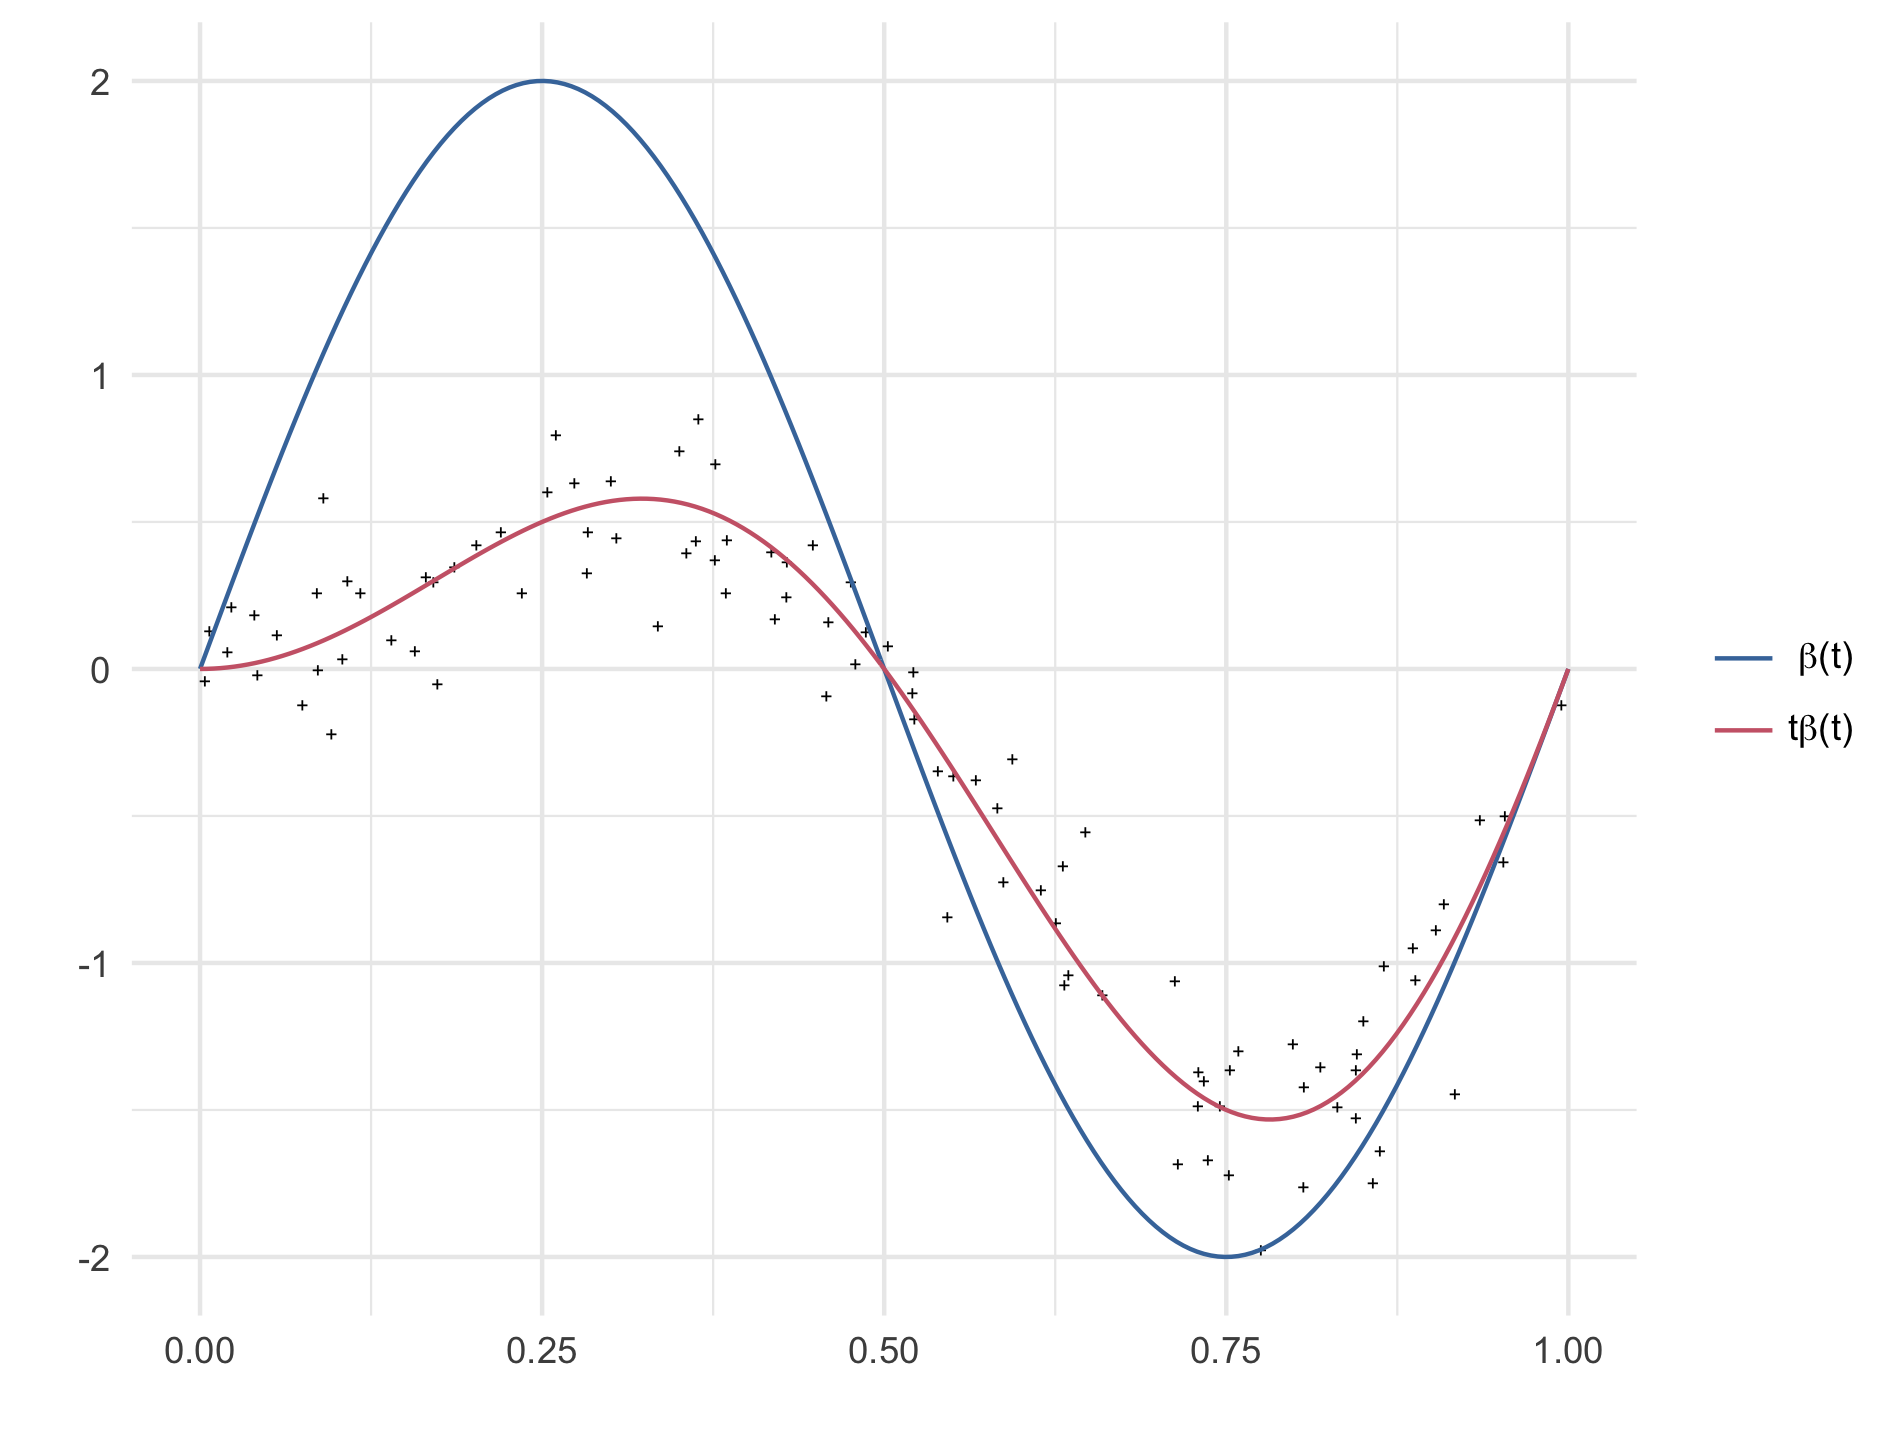
\includegraphics[scale=0.25]{PS_VCM_section_figure_1.png}
\caption{\textit{100 simulated data points where} $y\left(t\right) = t \beta\left( t \right) + 0.2\epsilon\left(t\right)$ \textit{where} $\epsilon$ \textit{is a white noise process with unit variance, and} $\beta\left(t\right) = 2\sin\left(2\pi t\right)$.}
\label{fig:PS_VCM_section_figure_1}
\end{figure}

\begin{figure}[H]
 \begin{subfigure}{.48\textwidth}
  \centering
   \graphicspath{{img/}}
 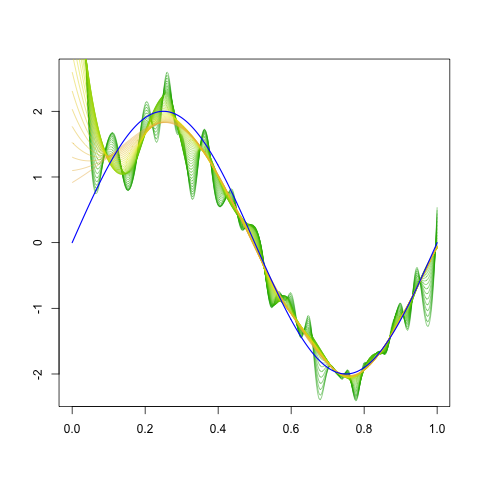
\includegraphics[scale=0.5]{PS_VCM_section_figure_2.png}
 \caption{$\hat{\beta}\left(t\right)$}
 \end{subfigure}
 \begin{subfigure}{.48\textwidth}
  \centering
   \graphicspath{{img/}}
  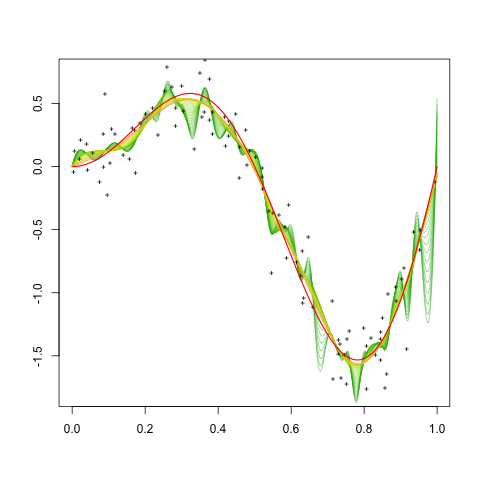
\includegraphics[scale=0.5]{PS_VCM_section_figure_3.png}
 \caption{$\hat{\mu}\left(t\right) = t \hat{\beta}\left(t\right)$}
\label{fig:PS_VCM_section_figure_2}
 \end{subfigure}
 \caption{\textit{Estimated coefficient function} $\hat{\beta}\left(t\right)$ \textit{and mean curve} $\hat{\mu}\left(t\right) = t \sin(2 \pi t)$ \textit{using a 80 B-splines basis functions of order 5 and a difference penalty of order} $k=3$.}
\end{figure}

The properties discussed in Section~\ref{BS_properties_continued} allude to how controlling the coefficients of a spline $f \in \mathscr{S}_{k,t}$ influences the shape of the overall function. Specifically, the form of the $j^{th}$ derivative provides an avenue of understanding how the differenced B-spline coefficient sequence is related to the volatility of the function on a given interval of its domain. The following figure visually explore the impact of the squared distance on adjacent basis coefficients on the function; a useful way of examining at P-splines is to consider the coefficients as the skeleton of the function, then draping the B-splines over them to put the flesh over the bones. A smoother sequence of coefficients leads to a smoother curve, which is clearly illustrated in Figure~\ref{fig:second_ord_PS_pen_SML_lambda}. As long as the coefficient sequence is smooth, the number of basis functions (and coefficients) is unimportant. The penalty ensures the smoothness of the skeleton.

\begin{figure}[H]
\begin{subfigure}{.5\textwidth}
  \centering
   \graphicspath{{img/}}
  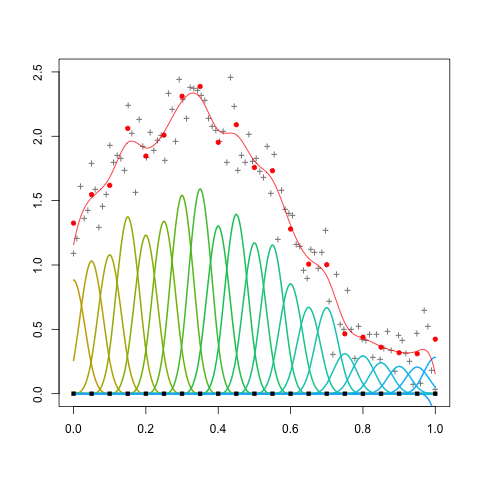
\includegraphics[scale=0.5]{pspline_pord2_xsmall_lambda.png}
  \label{fig:pspline_small_lambda}
\end{subfigure}
\begin{subfigure}{.5\textwidth}
  \centering
   \graphicspath{{img/}}
  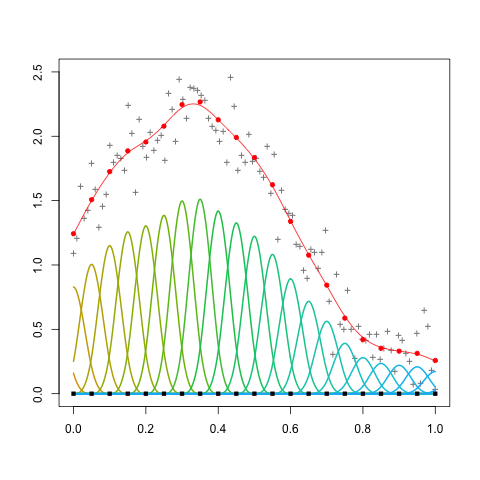
\includegraphics[scale=0.5]{pspline_pord2_small_lambda.png}
  \label{fig:pspline_small_lambda}
\end{subfigure}
\begin{subfigure}{.5\textwidth}
  \centering
   \graphicspath{{img/}}
  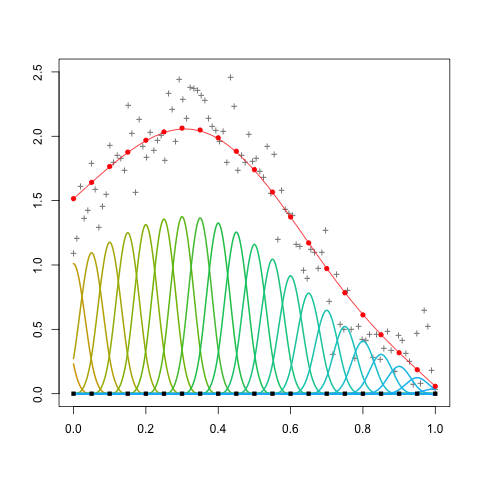
\includegraphics[scale=0.5]{pspline_pord2_medium_lambda.png}
  \label{fig:pspline_small_lambda}
\end{subfigure}
\begin{subfigure}{.5\textwidth}
  \centering
   \graphicspath{{img/}}
  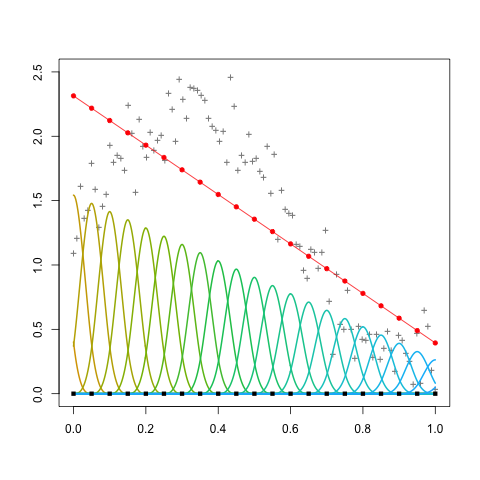
\includegraphics[scale=0.5]{pspline_pord2_large_lambda.png}
  \label{fig:pspline_small_lambda}
\end{subfigure}
\caption{\textit{Illustration of the impact of the second order difference penalty. The number of B-splines used is the same in each plot, with the value of the penalty parameter increasing from left to right and top to bottom across each plot. The fitted curve in the upper left plot is the most ``wiggly'' of any of the fits, as the penalty plays the weakest roll in the fitted coefficients there. The red circles are the values of each of the B-spline coefficients; as the penalty increases, they form as smoother sequence as we move across the four plots, which results in a smoother fitted function. As the penalty parameter approaches infinity, the fit approaches a linear function as shown in the bottom right plot.}}
\label{fig:second_ord_PS_pen_SML_lambda}
\end{figure}

The number of B-splines can be much larger than the number of observations because penalty ensures that the fitting procedure well-conditioned. One could literally use a thousand splines to fit ten observations without problems. Figure~\ref{fig:overcomplete_basis_pspline} illustrates this utility of the penalty for simulated data. There are $m=10$ observations and $40 + 3$ cubic B-splines. This property of P-splines cannot be overly appreciated, as it allows us to completely circumvent the nontrivial task of the optimal selection of knot placement. But one simply cannot have too many B-splines. Unless computational constraints are of concern, which is possible with large models, it is prudent to use even more. Figure~\ref{fig:PS_penalty_section_figure_3} shows how the fitted function changes as the tuning parameter $\lambda$ is varied in the presence of sparsely sampled data. 

\begin{figure}[H]   \label{fig:overcomplete_basis_pspline}
  \centering
   \graphicspath{{img/}}
  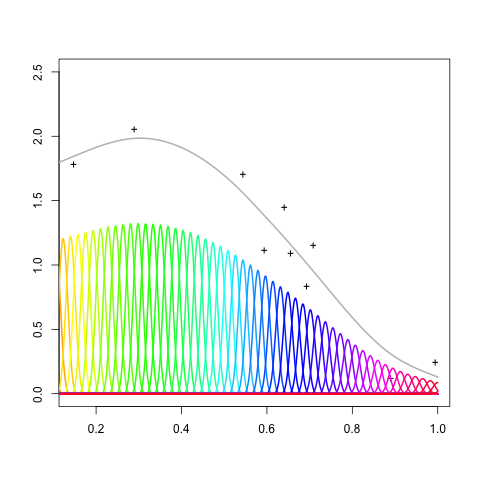
\includegraphics[scale=0.75]{pspline_10obs_60_basis_functions.png}
  \caption{P-spline smoothing of 10 observations using 60 B-spline basis functions.}
\end{figure}

\begin{figure}[H] \label{fig:PS_penalty_section_figure_3}
\centering
 \graphicspath{{img/}}
  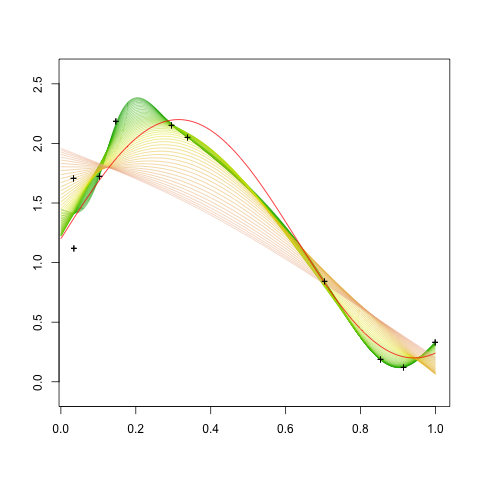
\includegraphics[width=4in, height=4in]{PS_penalty_section_figure_3.png}

  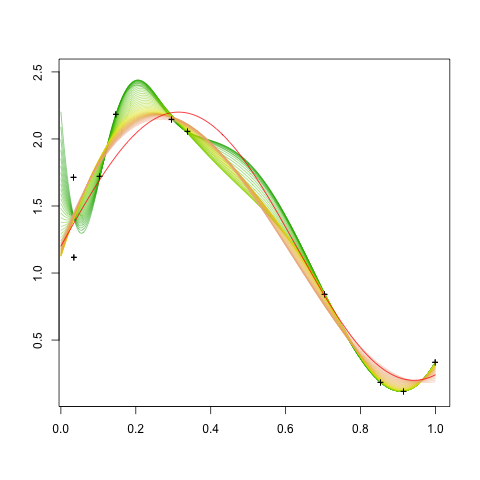
\includegraphics[width=4in, height=4in]{PS_penalty_section_figure_4.png}
 \caption{Fitted mean curves using a second (top) and third (bottom) order difference penalty for simulated data, sparsely sampled along the indexing variable: $y\left(t\right) = 1.2 + \sin\left(5t\right) + 0.2\epsilon_t$, where $\epsilon_t \stackrel{i.i.d.}{\sim}\textup{N}\left(0,1\right)$. A total of 10 data points were fit using a basis of 60 B-splines of degree $k=3$.}
\end{figure}

%%==============================================================================================================================================
%%==============================================================================================================================================
%%==============================================================================================================================================
%%==============================================================================================================================================
%%==============================================================================================================================================
%%==============================================================================================================================================
\subsection{Properties of P-splines}
% \subfile{chapter-3-subfiles/chapter-3-properties-of-psplines}

P-splines exhibit a number of advantageous properties, many of which are due to the inherited properties of the B-spline basis functions.

\begin{enumerate} \label{eq:PS_properties}
\item \begin{description}\item[Boundary effects]
 P-splines show no boundary effects, as many types of kernel smoothers do. By this, we mean the spreading of a fitted curve or density outside of the (physical) domain of the data, generally accompanied by bending toward zero.
\end{description}
\item \begin{description}\item[P-splines fit polynomial data exactly.] 
P-splines can fit polynomial data exactly. Given data $\left(t_i,y_i\right)$, if the $y_i$ are a polynomial in $t$ of degree $k$, then B-splines of degree $k$ or higher will fit the data exactly. 
\begin{proof}
This statement is equivalent to the claim that given $\xi = \left\{ \xi_i \right\}$, $i=1,\dots,l+1$, and $g$ such that $y\left(t\right) = g\left(t\right)$, we can find an $f \in \PP_{k,\xi} \bigcap \mathscr{C}^{\left(k-2\right)}$ which agrees with $g$ at the points $\tau_1 < \dots < \tau_n$  with $\tau_i \in \left[\xi_1,\xi_{l+1}\right]$ for all $i$, where
\[
n=k+l-1
\]
The solution, $f$ is constructed as follows: generate the knot sequence $t = \left\{t_i\right\}$ as per the recipe in Theorem~\ref{curryschoenbergthm}:
\begin{align*}
t_1 &= t_2 = \dots = t_k = \xi_1 & \\
t_{k+i} &= \xi_{i+1}, & i=1,\dots,l-1\\
t_{n+1} &= t_{n+2} = \dots = t_{n+k} = \xi_{l+1} & 
\end{align*}

Let $\left\{ B_{ik} \right\}$, $i=1,\dots,n$ be the corresponding sequence of B-splines of order $k$, which are a basis for $\PP_{k,\xi} \bigcap \mathscr{C}^{\left(k-2\right)}$ by Theorem~\ref{curryschoenbergthm}. Here, $\PP_{k,\xi} \bigcap \mathscr{C}^{\left(k-2\right)}$ denotes the space of pp functions with breakpoints $\xi$ having two continuous (global) derivatives. Then, \cite{schoenberg1953polya} have shown that there exists exactly one $f \in \PP_{k,\xi} \bigcap \mathscr{C}^{\left(k-2\right)}$ agreeing with $g$ at $\tau_1,\dots, \tau_n$ if and only if 
\[
B_{ik}\left(\tau_i\right) \ne 0, \qquad \qquad i=1,\dots,n.
\]
This $f$ has a unique expansion of the form
\[
f = \sum_{i=1}^n a_i B_{ik}
\] 
for coefficients $a_i,\dots, a_n$, which are the solution to the linear system
\[
\sum_{j=1}^n a_jB_{jk}\left(\tau_i\right) = g\left(\tau_i\right), \qquad \qquad i=1,\dots,n.
\]
This system has a banded matrix of coefficients since $B_{jk}\left(\tau_i\right) \ne 0$ if and only if $\tau_i \in \left[t_j,t_{j+k}\right]$. So if $B_{jk}\left(\tau_i\right) \ne 0$ and thus $\tau_i \in \left(t_j,t_{j+k}\right)$, then there are at most $k$ of the $j$ indices such that $B_{jk}\left(\tau_i\right)$ is nonzero. And further, each of these indices $j$ must be such that 
\[
\left(t_i,t_{i+k}\right) \bigcap \left(t_j,t_{j+k}\right) \ne \emptyset,
\]
or such that $\vert i-j \vert < k$. At worst, the system corresponds to a banded matrix with $k-1$ lower and $k-1$ upper diagonals. 
\end{proof}
The same is true for P-splines if the order of the penalty is $k+1$ or higher, irrespective of the value of $\lambda$. Consider imposing a first-order difference penalty and a fit to data $y$ that is constant - a polynomial of degree 0. Since 
\[
\sum_{j=1}^n \hat{\alpha}_j B_j\left( x_i \right) = c, 
\]
\noindent
we have that
\[
\sum_{j=1}^n \hat{\alpha}_j B^\prime_j\left( x \right) = 0, 
\]
\noindent
for all $x$. From the relationship between differences and derivatives in \ref{eq:more_BS_properties} \ref{eq:BS_deriv_property}, 

\[
0 = \sum_{j=1}^n B^\prime_{j,k}\left(x\right) = \sum_{j=1}^n \Delta\alpha_{j+1} B_{j,k-1}\left( x \right), 
\]
\noindent
so that we must have $\Delta \alpha_j = 0$ for all $j$, and 
\[
\sum_{j=2}^n \Delta \alpha_j = 0.
\]

This shows that the penalty has no impact on the basis coefficients, and the resulting fit is identical to that when using unpenalized B-splines. Using induction, one can show that this is also true when the relationship between $x$ and $y$ is linear and a second order difference penalty is used, and for any values of the polynomial order and order of the difference penalty.\end{description}
\item \begin{description}\item[Null models under difference penalties] \label{eq:PS_property_3}
The limiting P-spline fit approaches a polynomial under strongly enforced smoothing. As $\lambda \rightarrow \infty$, under a difference penalty of order $d$, the fitted function will approach a polynomial of degree $d-1$ as long as the degree of the B-splines is greater than or equal to $k$. To see this, we again need to use the relationship between the differenced coefficient sequence and the derivative of a B-spline as described in \ref{eq:more_BS_properties} \ref{eq:BS_deriv_property}. Consider using the second-order difference penalty; when $\lambda$ is large, the penalty dominates the P-spline objective function defined in \ref{eq:S_pen_varying_intercept_model}, so that the minimizer $\alpha$ must be such that $\sum_{j=3}^n\left(\Delta^2\alpha_j\right)^2$ is close to zero. Consequently, each of the individual second differences must also be nearly zero, and thus the second derivative of the fitted function must be close to zero over the entire domain.
\end{description}
\item \begin{description}\item[The limiting behaviour of $H_\lambda$] The trace of the hat matrix, 
\[
H_\lambda = B\left(B^TB + \lambda D_k^TD_k\right)^{-1}B^Ty
\] 
(or for $H$ defined for the addition of a varying slope component as in \ref{eq:simplest_VC_model_hat_matrix}) approaches $k$, the order of the differencing operator, as $\lambda$ increases. We index $H$ with the smoothing parameter to indicate that the elements of $H$ are a function of $\lambda$. Let
\begin{equation}
Q_B = B^T B \qquad \mbox{and} \qquad Q_\lambda = \lambda D^T D.
\end{equation}
Then using properties of the matrix trace, we can write
\begin{align}
\begin{split}
\mbox{tr}\left(H_\lambda \right) &= \mbox{tr}\bigg[ \left(Q_B + Q_\lambda \right)^{-1}Q_B \bigg]\\
&=\mbox{tr}\bigg[ Q_B^{1/2}\left(Q_B + Q_\lambda \right)^{-1}Q_B^{1/2} \bigg] \\
&=\mbox{tr}\bigg[\left(I + Q_B^{-{1/2}}Q_\lambda Q_B^{-{1/2}} \right)^{-1} \bigg]
\end{split}
\end{align}
Define $L \equiv Q_B^{-{1/2}}Q_\lambda Q_B^{-{1/2}}$. Then
\begin{equation}
\mbox{tr}\left(H_\lambda \right) = \mbox{tr}\bigg[\left(I + \lambda L \right)^{-1} \bigg] = \sum_{j=1}^n \frac{1}{1 + \lambda \gamma_j}
\end{equation}
 where $\gamma_j$, $j=1,\dots,n$ are the eigenvalues of $L$. $Q_\lambda$ has exactly $k$ eigenvalues equal to zero, hence $L$ has $k$ zero eigenvalues. For large $\lambda$, only the $k$ terms with $\gamma_j=0$ contribute to the sum which gives the trace of $H$, so that
 \[
\lim_{\lambda \rightarrow \infty  } \mbox{tr}\left(H\right) = k.
 \]
\end{description}
\end{enumerate}

The previous derivations hold regardless of whether we are fitting the varying intercept-only model, with $\mu\left( t\right) = \beta_0\left(t\right)$ or accommodating a varying slope for a regressor by specifying $\mu\left( t\right) = \beta_0\left(t\right) + \beta_1\left(t\right)x\left(t\right)$. The inspection of the hat matrix $H$ is a prelude to the following section, where we will discuss how to use the properties of $H$ to tune the smoothing parameter for optimal model selection. We will later show that extension of these results can be extended in a rather straightforward manner to the case that is of our particular interest: when the smooth slope function is a two-dimensional surface rather than a curve.

\begin{figure}[H]
\begin{subfigure}{.5\textwidth}
  \centering
   \graphicspath{{img/}}
  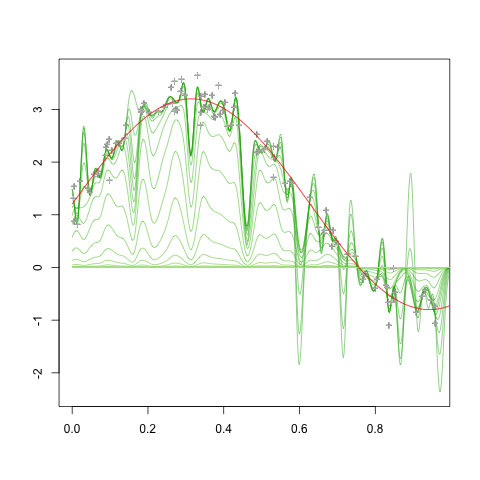
\includegraphics[scale=0.5]{PS_penalty_section_figure_6_order_0.png}
  %\label{fig:pspline_small_lambda}
\caption{$d=0$ }
\end{subfigure}
\begin{subfigure}{.5\textwidth}
  \centering
   \graphicspath{{img/}}
  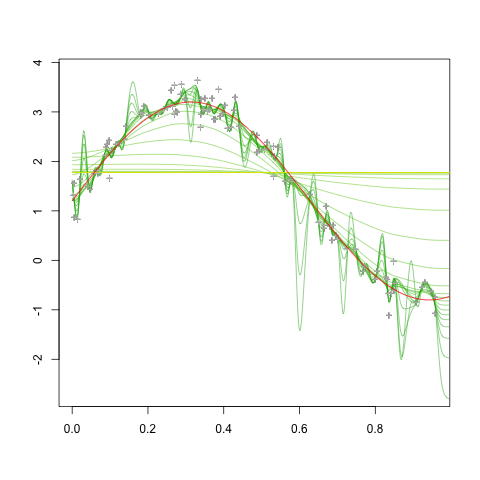
\includegraphics[scale=0.5]{PS_penalty_section_figure_6_order_1.png}
 % \label{fig:pspline_small_lambda}
\caption{$d=1$}
\end{subfigure}
\begin{subfigure}{.5\textwidth}
  \centering
   \graphicspath{{img/}}
  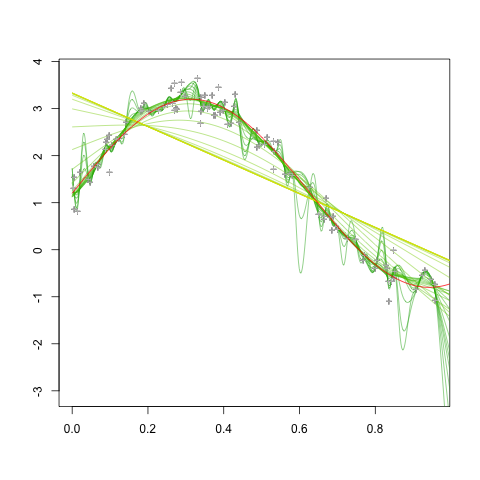
\includegraphics[scale=0.5]{PS_penalty_section_figure_6_order_2.png}
  %\label{fig:pspline_small_lambda}
\caption{$d=2$}
\end{subfigure}
\begin{subfigure}{.5\textwidth}
  \centering
   \graphicspath{{img/}}
  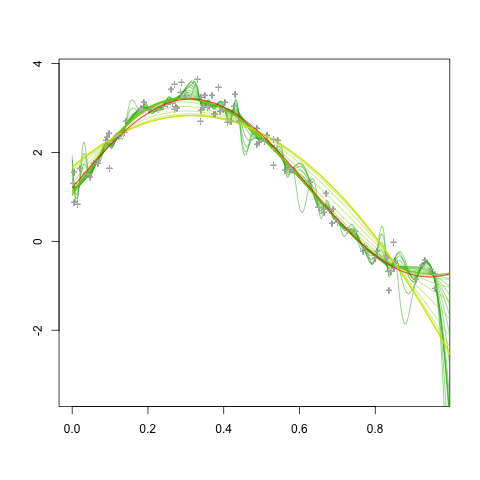
\includegraphics[scale=0.5]{PS_penalty_section_figure_6_order_3.png}
  %\label{fig:pspline_small_lambda}
\caption{$d=3$}
\end{subfigure}
\caption{\textit{Illustration of the impact of the order of the difference penalty. The number of B-splines used is the same in each plot, with the penalty parameter varying from across the same grid of values. The fitted curves in the upper left plot correspond to the difference penalty of order $0$, where $\vert D_0 \alpha \vert^2 = \sum_{i=1}^n \alpha_i^2$, analogous to ridge regression using the B-spline basis as regression covariates. The fitted curves approach polynomials of degree $d-1$ as $\lambda \rightarrow \infty$, as discussed in \ref{eq:PS_properties} \ref{eq:PS_property_3}.}}
\label{fig:PS_penalty_section_figure_6}
\end{figure}

\begin{figure}[h]
\centering
 \graphicspath{{img/}}
  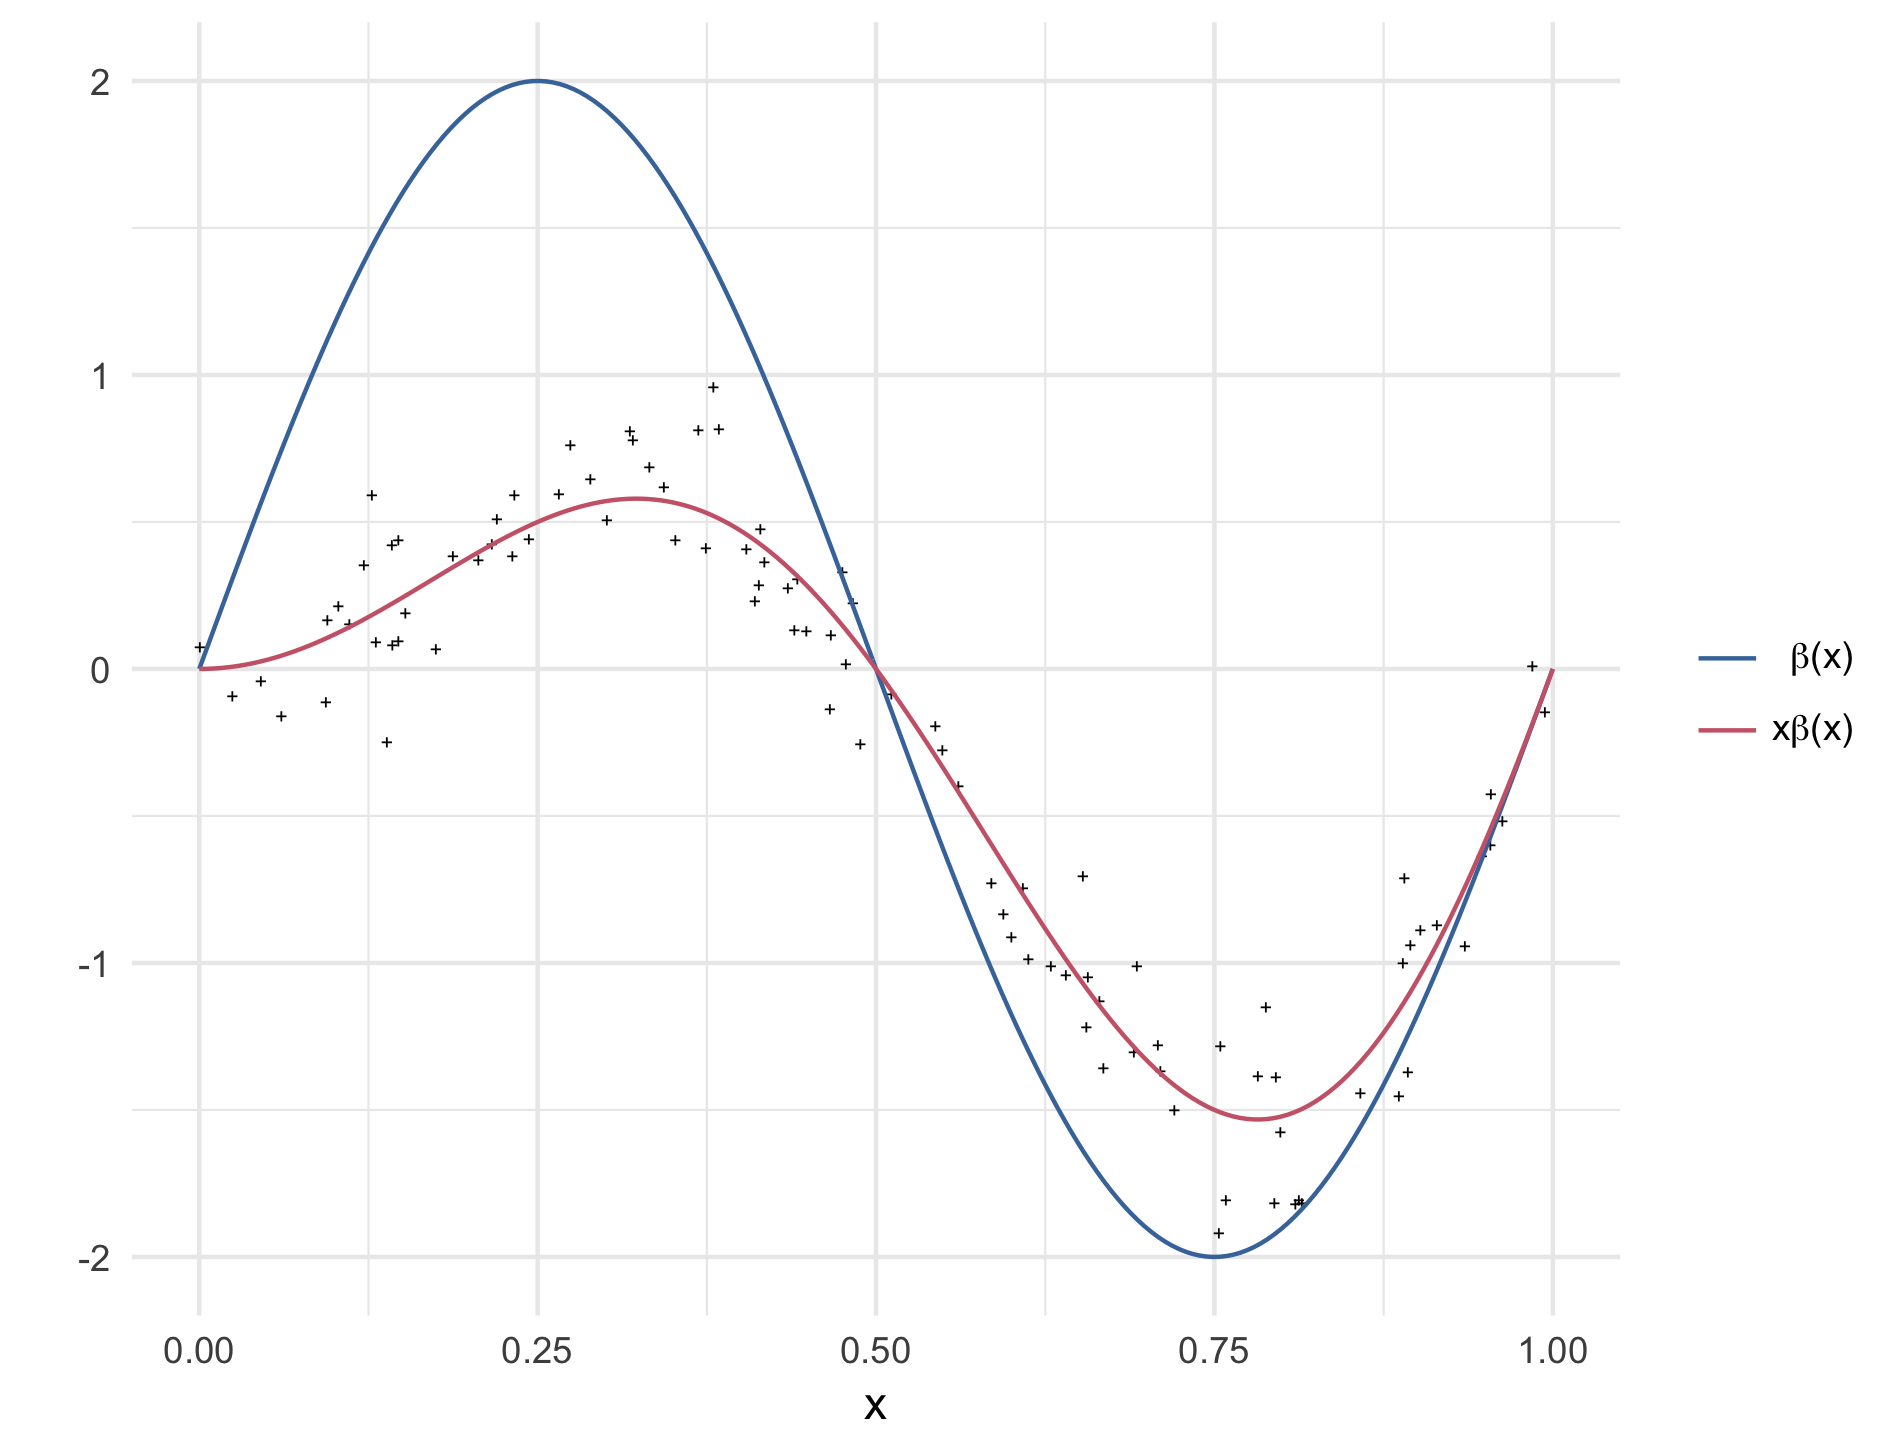
\includegraphics[width=4in, height=4in]{PS_penalty_section_figure_5.png}
 %\caption{Tensor product of two cubic B-splines}
\end{figure}
%%==============================================================================================================================================
%%==============================================================================================================================================
%%==============================================================================================================================================
%%==============================================================================================================================================
%%==============================================================================================================================================
%%==============================================================================================================================================

%%==============================================================================================================================================
%%==============================================================================================================================================
%%==============================================================================================================================================
%%==============================================================================================================================================
%%==============================================================================================================================================
%%==============================================================================================================================================
\subsection{The reguarlized MLE for $\phi$ via tensor product P-splines}
% \subfile{chapter-3-subfiles/chapter-3-tensor-product-pspline-MLE}
We equip the $l$ and $m$ axes each with a B-spline basis to construct a basis for the varying coefficient function $\phi$ in \ref{eq:phi-star} by taking the tensor product of the two marginal bases. Let 
\[
B_{1}\left(l\right),\dots, B_{K}\left(l\right)  \mbox{ and } B_{1}\left(m\right),\dots, B_{L}\left(m\right)
\]
denote the B-spline bases for $l$ and $m$, each having a set of equally spaced knots along their respective domain. It is worth noting that while we have chosen not to distinguish between $\left\{ B_k \right\}$ and $\left\{ {B}_l \right\}$ for the sake of brevity, one is free to specify a different basis for each dimension either by using different order B-spline or, of course, using different numbers of knots, and hence entirely different knot sequences since P-splines rely on bases with equally spaced knots. The tensor product basis functions
\begin{equation*}
T_{jk}\left(l,m\right) = B_j\left(l\right){B}_k\left(m\right)
\end{equation*}
\noindent
carve the $l$-$m$ domain into rectangles.  Figure~\ref{fig:sparse_bicubic_BS_basis} shows a thinned tensor product basis $\left\{ T_{kl} \right\}$; a portion of the basis was omitted to eliminate overlapping of the basis functions so that the reader can identify individual tensor products. Each ``hill'' in Figure~\ref{fig:sparse_bicubic_BS_basis} is associated with an unknown coefficient $\theta_{ij}$ which determines the height of the hill. For a given knot grid, we can approximate a surface by

\begin{equation} \label{eq:varying-coefficient-tensor-product-expansion}
\phi\left(l,m\right) = \sum_{i=1}^K \sum_{j=1}^L \theta_{ij} B_{i}\left(l\right) B_{j}\left(m\right), 
\end{equation}
\noindent
and the function evaluated at the observed $\left(l_{ijk}, m_{ijk}\right)$ may be written 
\begin{equation*} 
\vphistar = B_m \Theta B_l^\prime
\end{equation*}
\noindent 
where $\Theta$ denotes the $K \times L$ matrix of tensor product coefficients, with elements $\theta_{ij}$.

\begin{figure}[H]
\centering
 \graphicspath{{img/}}
  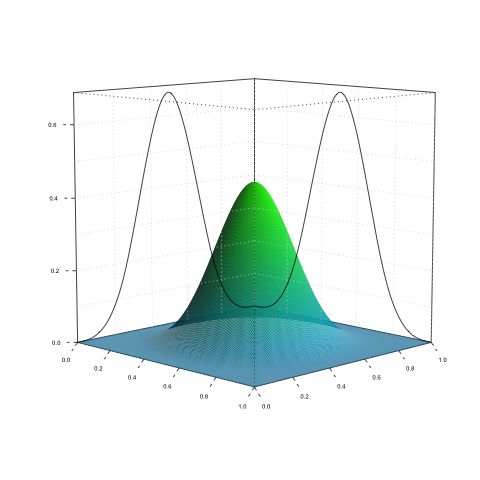
\includegraphics[width=4in, height=4in]{bicubic_basis_function.png}
 
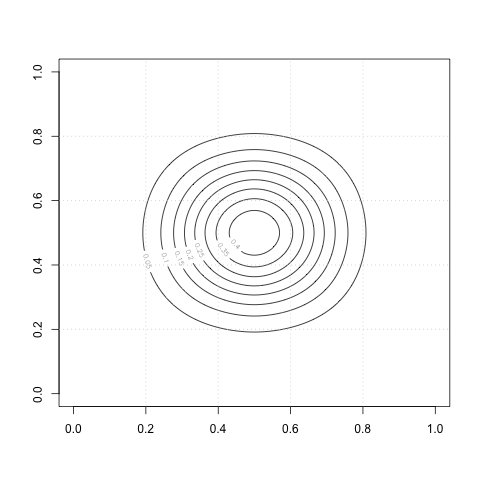
\includegraphics[width=4in, height=4in]{bicubic_bspline_contour.png}
\caption{Tensor product of two cubic B-splines}
\label{fig:bicubic_BS}
\end{figure}

\begin{figure}[H]
  \centering
  \graphicspath{{img/}}
  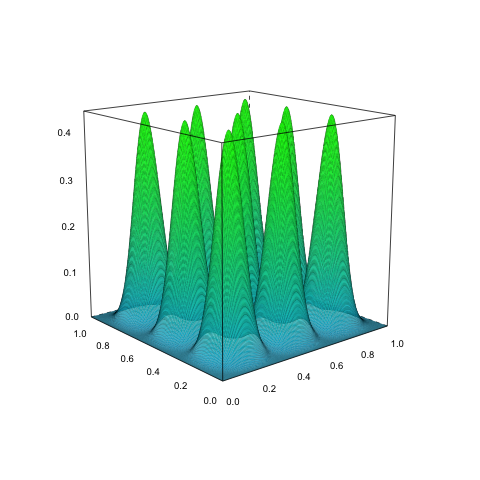
\includegraphics[width=5in,height=5in]{sparse_bicubic_basis.png}
  \caption{A subset of a full bivariate basis of cubic B-splines}\label{fig:sparse_bicubic_BS_basis}
\end{figure}

\subsection{Regularization with difference penalties} \label{subsection:univariate-psplines}

The minimizer of \ref{eq:loglikelihood} honors the fidelity to the data, so to balance the complexity of the fitted function with the goodness of fit to the data, we can append a penalty to the negative log likelihood to control the fitted function. By using rich B-spline bases for $l$ and $m$ alongside discrete difference penalties on the spline coefficients, we can achieve as much smoothness of the fitted function in both the $l$ and $m$ dimensions as desired. \cite{o1986statistical} was the first to propose using a rich B-spline basis and using a penalty to restrict the flexibility of the fitted curve, like \cite{wahba1990spline} applying a penalty to the second derivative of the fitted curve:
\[
J = \int_0^1 \left[ f^{\prime \prime}\left(l\right)\right]^2\;dx.
\]

For a B-spline of the form
\[
f\left(x\right) = \sum\limits_{j=1}^n \theta_i B_j\left(x\right),
\]
one can derive a banded matrix $P$ using the properties of B-splines such that 
 \[
 J = \theta^\prime P \theta
 \] 
 \noindent
 where $\theta = \left(\theta_1,\dots, \theta_n\right)$. The $i$-$j^{th}$ element of $P$ is given by
 \[
 p_{ij} = \int_0^1 B_i^{\prime \prime} \left( x \right)B_j^{\prime \prime} \left( x \right)\;dx.
 \]

%As discussed in Section 2, we can define an entire class of functional autoregressive models using only the $l$ direction, and additionally, as discussed in Section 3, there is a natural expectation about the functional form of the autoregressive coefficient function (and hence covariance) as a function of $l$. The use of smoothing splines to estimate $\phi$ outlined in Section~\ref{} yields smooth null models, but smoothness of the elements of the Cholesky factor alone may not lead to desirable structure in the inverse covariance matrix.  

%
%These approaches implicitly adopt different notions of sparsity. Like \cite{huang2006covariance} and \cite{levina2008sparse}, our aim is to regularize the inverse of the covariance matrix through the Cholesky factor. Expressing the varying coefficient function using a tensor product basis expansion builds the foundation for a flexible estimation framework within which employing multiple notions of smoothness is simple and straightforward. 
%

In some applications, it is useful to work with third and fourth order differences, since for large values of $\lambda$, the fitted curve approaches a parametric polynomial model. This may be of particular interest in the context of estimating the elements of the Cholesky factor, as many have proposed simple parametric functions of lag only for $\phi$, such as low order polynomials. See \cite{pourahmadi1999joint}. However, with the use of higher order derivatives, the computation of $P$ is nontrivial and becomes very tedious. \cite{eilers1996flexible} were the first to propose P-splines, or \emph{penalized B-splines}, as an approach to nonparametric regression. P-splines circumvent complexity associated with constructing such penalty matrices by omitting derivatives and integrals altogether, replacing them with finite differences and sums. 

Instead, flexibility of the fitted function is controlled by using a discrete penalty matrix based on finite difference formulas. Smoothness of the fitted function is achieved by first using a rich B-spline basis with equally spaced knots to purposefully overfit the smooth coefficient vectors; this eliminates the difficulty of choosing the optimal set of knots. Then by attaching a difference penalty to the goodness of fit measure, one may prevent overfitting and make a potentially ill-conditioned fitting procedure a well-conditioned one. The finite difference penalty is simple to compute and can be handled mechanically for any order of the differences. Since it is easily introduced into regression equations, it is feasible to evaluate the impact of different orders of the differences on the fitted model.  Using the properties of B-splines, it is straightforward to show that the difference penalty of order $d$ is a good discrete approximation to the integrated square of the $d^{th}$ derivative, so little is lost by replacing the derivative-based penalty with

\begin{equation} \label{eq:bspline-difference-penalty}
J_d\left( f \right) = \sum_{j=d}^n \left(\Delta^d \theta_j\right)^2
\end{equation} 
\noindent
where $\theta = \left( \theta_1,\dots,\theta_n \right)$. Let $D_d$ denote the matrix difference operator: $D_d\theta = \Delta^d \theta$, where

 \begin{align*}
 \Delta \theta_j &= \theta_j - \theta_{j-1}, \quad  \Delta^2 \theta_j = \Delta\left(\Delta \theta_j\right) = \theta_j - 2\theta_{j-1} + \theta_{j-2}
 \end{align*}
\noindent 
In general,
\begin{equation*}
\Delta^d \theta_j = \Delta\left(\Delta^{d-1} \theta_j \right).
\end{equation*} 
\noindent
Then, \ref{eq:bspline-difference-penalty} can be written in terms of the squared norm of the difference operator applied to the vector of B-spline coefficients:
\begin{align} 
\begin{split} \label{eq:bspline-difference-penalty-vector-form}
J_d\left( f \right) &= \vert \vert D_d\theta \vert \vert^2 \\
&= \theta^\prime P_d \theta
\end{split}
\end{align}
\noindent
where $P_d = D_d^\prime D_d$.  To examine the connection between the second-derivative penalty to the penalty on second-order differences of the B-spline coefficients, we only need to employ straightforward calculus and exploit the recursive property of the B-spline basis functions:

\begin{equation*} 
\int_0^1 \left[ f^{\prime \prime}\left(x\right)\right]^2\;dx = \int_{0}^{1} \left\{ \sum\limits_{j=1}^n  \theta_j B_{j,3}^{\prime \prime} \left(l\right) \right\}^2\; dl.
\end{equation*}
\noindent
The derivative properties of B-splines permits this to be written as 
\begin{equation*} \label{eq:second-derivative-bspline-penalty}
\int_0^1 \left[ f^{\prime \prime}\left(x\right)\right]^2\;dx =  \int_{0}^{1}  \bigg[ \sum\limits_{j=1}^n \sum\limits_{k=1}^n \Delta^2 \theta_j \Delta^2 \theta_k B_{j,1}\left(l\right)B_{k,1}\left(l\right)\bigg]\; dl  . 
\end{equation*}
\noindent
Most of the cross products of $B_{j,1}\left(x\right)$ and $B_{k,1}\left( x \right)$ vanish since B-splines of degree 1 only overlap when $j$ is $k-1$, $k$, or $k+1$. Thus, we have that
\begin{align}
\begin{split}
\int_0^1 \left[ f^{\prime \prime}\left(x\right)\right]^2\;dx  = {} &  \int_0^1 \bigg[ \left\{ \sum\limits_{j=1}^n   \Delta^2 \theta_j  B_j\left(l,1\right)  \right\}^2  + 2 \sum_{j}\Delta^2 \theta_j\Delta^2 \theta_{j-1}B_j\left(l,1\right)B_{j-1}\left(l,1\right) \bigg]\; dl \\ 
= {} & \sum \limits_{j=1}^n  \left( \Delta^2\theta_j \right)^2 \int_0^1 B_j^2\left(l,1\right)\;dl \\
   &{} \;\;\;\;\;\;\;\;\;\;\;\;\;\;\;\;\;\; + 2 \sum\limits_{j=1}^n \Delta^2 \theta_j\Delta^2 \theta_{j-1} \int_0^1 B_j\left(l,1\right)B_{j-1}\left(l,1\right)\;dl 
\end{split}
\end{align}
\noindent
which can be written as
\begin{equation} \label{eq:derivative-penalty-difference-penalty-connection}
\int_0^1 \left[ f^{\prime \prime}\left(x\right)\right]^2\;dx  = c_1 \sum\limits_{j=2}^n \left( \Delta^2 \theta_j\right)^2 + c_2 \sum\limits_{j=3}^n \Delta^2 \theta_j\Delta^2 \theta_{j-1}
\end{equation}
\noindent
Given a set of equidistant knots, the constants $c_1$ and $c_2$ are given by
\begin{equation}
\begin{split}
c_1 & =   \int_0^1 B_{j,1}^2\left(x\right) dx\\
c_2 & = \int_0^1 B_{j,1}\left(x\right)B_{j-1,1}\left(x\right) dx.
\end{split}
\end{equation}

This gives us that the traditional smoothness penalty on the squared second derivative can be written as a linear combination of a penalty on the second-order differences of the B-spline coefficients \ref{eq:bspline-difference-penalty} and the sum of the cross products of neighboring second differences. The second term in \ref{eq:derivative-penalty-difference-penalty-connection} leads to a complex objective function when minimizing the penalized likelihood, where seven adjacent spline coefficients occur, as opposed to five if only the first term in \ref{eq:derivative-penalty-difference-penalty-connection} is used in the penalty. The added complexity is a consequence of overlapping B-splines, which quickly increases when using higher order differences and higher order B-splines. We can seamlessly augment the likelihood with the difference penalty to achieve smooth fitted functions without the complexity posed by the derivative-based penalty.
%citet{chen2011efficient}, citet{pourahmadi1999joint}, and citet{pourahmadi2002dynamic} have elicited parametric models for the generalized autoregressive coefficients, letting the GARPs depend only on the distance between two time points.

A smoother sequence of coefficients leads to a smoother curve, as illustrated in Figure~\ref{fig:second_ord_PS_pen_SML_lambda}.  The relationship between P-spline curves and their coefficients is easily characterized if we consider the coefficients as the skeleton of the function, and draping the B-splines over them puts the flesh on the bones. As long as the coefficient sequence is smooth, the number of basis functions (and coefficients) is unimportant since the penalty ensures the smoothness of the skeleton and that the fitting procedure is well-conditioned. Figure~\ref{fig:overcomplete_basis_pspline} illustrates this utility of the penalty for simulated data; there are $m=10$ observations and $60$ cubic B-splines. This property of P-splines cannot be overly appreciated because it frees us from the concern of choosing the optimal set of knots. Unless computational constraints are of concern, which is possible with large models, it is prudent to use even more B-splines. Figure~\ref{fig:PS_penalty_section_figure_2} shows how the fitted function changes as the tuning parameter varies when the data are sparsely sampled. P-splines enjoy a number of additional advantageous properties, many of which are inherited from the attractive properties of B-splines. See \cite{eilers1996flexible}  for a detailed presentation. 

\begin{figure}[H] \label{fig:PS-smoothing-figure-1}
\begin{subfigure}{.5\textwidth}
  \centering
   \graphicspath{{img/}}
  \includegraphics[scale=0.5]{pspline_pord2_xsmall_lambda.png}
  \label{fig:pspline_small_lambda}
\end{subfigure}
\begin{subfigure}{.5\textwidth}
  \centering
   \graphicspath{{img/}}
  \includegraphics[scale=0.5]{pspline_pord2_small_lambda.png}
  \label{fig:pspline_small_lambda}
\end{subfigure}
\begin{subfigure}{.5\textwidth}
  \centering
   \graphicspath{{img/}}
  \includegraphics[scale=0.5]{pspline_pord2_medium_lambda.png}
  \label{fig:pspline_small_lambda}
\end{subfigure}
\begin{subfigure}{.5\textwidth}
  \centering
   \graphicspath{{img/}}
  \includegraphics[scale=0.5]{pspline_pord2_large_lambda.png}
  \label{fig:pspline_small_lambda}
\end{subfigure}
\caption{\textit{Illustration of the impact of the second order difference penalty. The number of B-splines used is the same in each plot, with the value of the penalty parameter increasing from left to right and top to bottom across each plot. The fitted curve in the upper left plot is the most ``wiggly'' of any of the fits, as the penalty plays the weakest roll in the fitted coefficients there. The red circles are the values of each of the B-spline coefficients; as the penalty increases, they form as smoother sequence as we move across the four plots, which results in a smoother fitted function. As the penalty parameter approaches infinity, the fit approaches a linear function as shown in the bottom right plot.}}
\label{fig:second-ord-PS-pen-SML-lambda}
\end{figure}
%%==============================================================================================================================================
%%==============================================================================================================================================
%%==============================================================================================================================================
%%==============================================================================================================================================
%%==============================================================================================================================================
%%==============================================================================================================================================


%We employ maximum likelihood  for the estimation of  the varying coefficient function $\phi\left(t,s\right)$ and the innovation variance function $\sigma\left(t\right)$, though neither the derivation the form of model~\ref{eq:ARmodel} nor model~\ref{eq:MyModel} via the Cholesky decomposition rely on any assumptions about the distribution of $Y$. 
%
%For fixed $\left\{ \sigma_j^2 \right\}$, as a function of $\phi_{jk}$ the negative log-likelihood for a sample of $N$  i.i.d. observations $Y_1,Y_2,\dots,Y_N$ from a multivariate Gaussian distribution is proportional to the usual error sums of squares:
%
%\begin{equation}
%-2 L\left(y_1,\dots,y_N ,\phi \vert \vsigmasq \right) \propto \sum_{i=1}^N \sum_{j=2}^{m_i} \sigma\left({t_j}\right)^{-2} \left(y_{ij} - \sum_{k=1}^{j-1}\phi\left({t_{ij},t_{ik}}\right)y_{ik} \right)^2 \label{loglikelihood}
%\end{equation}
%\noindent
%where 
%\[
%y_i = \left( y_{i1}, y_{i2}, \dots, y_{i,m_i}\right), \quad i=1,\dots,N 
%\] 
%
%%% explain here that we omit y_{i1} from the likelihood here because in the first stage of estimation (for $\phi$), the first observation in each vector doesn't contribute to the likelihood
%\noindent
%denotes the vector of observations for subject $i$ with corresponding measurement times 
%\[
%t_{i1} < t_{i2} < \dots < t_{i,m_i}.
%\]
%The form of the likelihood of $y_1,\dots,y_N$ indicates that we allow both the number of measurements as well as the observation times to varying across subjects. The $\left\{t_{ij} \right\}$ need not be evenly-spaced within or across individuals. Denote the innovation variance function evaluated at the vector of observed time points by $\vsigmasq$, and similarly let $\vphistar$ denote the resulting vector when evaluating $\phi$ at the observed grid of time points, transformed to the $l$-$m$ axis. Estimation of the varying coefficient function and the innovation variance function may be accomplished in an iterative fashion:
%
%\fbox{\parbox{\textwidth}{\begin{enumerate}
%\item Fix $\vsigmasq = \vsigmasq_0$;
%\item find $\widehat{\vphistar} = \underset{\vphistar}{\arg\max} -2 L\left(y_1,\dots,y_N ,\vphistar \vert \vsigmasq_0 \right)$.
%\item Fix $\vphistar= \widehat{\vphistar}$;
%\item find $\widehat{\vsigmasq} = \underset{\vsigmasq}{\arg\max} -2 L\left(y_1,\dots,y_N , \vsigmasq \vert \widehat{\vphistar} \right)$.
%\item Iterate until convergence.
%\end{enumerate}}}
%
%\vspace{0.5cm}


% 
%\section{\emph{Penalized maximum likelihood estimation}}
%
%\begin{enumerate}
%\item Fix $\sigma_{ij}^2 = \sigma_{ij0}^2$, $i=1,\dots,N$ ,$j=1,\dots,M$.
%\item Find $\phi_0 = \underset{\phi}{arg \; min} -2L_\phi\left(\phi, y_1,\dots, y_N \right) + \lambda J\left( \phi \right)$
%\item Fix $\phi = \phi_{0}$.
%\item Find  $\sigma_{0}^2 = \underset{\sigma^2}{arg\; min} -2L_\sigma^2\left(\sigma^2, y_1,\dots, y_N \right) + \lambda J\left( \sigma^2 \right)$
%\end{enumerate}
%
%\begin{adjustwidth}{-2cm}{-2cm}
%\begin{equation}
%-2 L_\phi\left(\phi, y_1, \dots,y_N \right) = \sum_{i=1}^N \sum_{j=2}^{m_i} \sigma_{ij0}^{-2} \left(y_{ij} - \sum_{k=1}^{j-1}\phi\left({t_{ij},t_{ik}}\right)y_{ik} \right)^2 \label{loglikelihood}
%\end{equation}
%\end{adjustwidth}
% 





% 
%\section{\emph{Smooth ANOVA models}}
%Decompose
%\begin{equation} \label{eq:SANOVA-model}
%\carrotorangemath{
%\phi\left(l,m\right) = \mu + \phi_1\left(l\right) + \phi_2\left(m\right) + \phi_{12}\left(l,m\right)},
%\end{equation} 
%so Model~\ref{eq:MyModel} becomes
%
%\begin{align*}  
%\begin{split}% \label{eq:expanded-ps-anova-vc-model}
% y\left(t_j \right)  = \sum_{k=1}^{j-1} \bigg[\mu + \phi_1\left(l_{jk}\right) +  &\phi_2\left(m_{jk}\right) \bigg.\\[-2ex]
%\bigg. &+ \phi_{12}\left(l_{jk},m_{jk}\right) \bigg]y\left(t_k\right)+ \sigma\left(t_j\right)e\left({t_j}\right)
%\end{split}
%\end{align*}
% 

% \begin{columns}
%\begin{column}{0.5\textwidth}
%Equip $l$ and $m$ with
%\begin{align*}
%B_{1}\left(l\right),\dots, B_{K}\left(l\right),\\
%B_{1}\left(m\right),\dots, B_{L}\left(m\right)
%\end{align*}
%to build
%\begin{equation*}
%T_{jk}\left(l,m\right) = B_j\left(l\right){B}_k\left(m\right)
%\end{equation*}
%  \end{column}
%\begin{column}{0.5\textwidth}  %%<--- here
%    \begin{center}
%    \begin{figure}
%    \graphicspath{{img/}}
% \includegraphics[width=4cm]{sparse_bicubic_basis}
% \caption{A ``thinned'' tensor product basis}
% \end{figure}
%     \end{center}
%\end{column}
%\end{columns}
%\vspace{0.3cm}
%\begin{equation*}
%\phi\left(l,m\right) = \sum_{i=1}^K \sum_{j=1}^L \theta_{ij} B_{i}\left(l\right) B_{j}\left(m\right)
%\end{equation*}
%
 
%The parameters of the functional autoregressive model given by \ref{eq:MyModel} define the elements of the precision matrix $\Omega$, rather than the elements of $\Sigma$ itself. It is well known that if we let $Y = \left(Y_1, \dots, Y_m\right)^\prime$ denote the random vector having joint distribution with mean zero and covariance matrix $\Sigma$, then the elements of $\Sigma^{-1}=\Omega$, $\left\{ \omega_{ij} \right\}$ may be interpreted as partial covariances between the elements of $Y$. This suggests shrinking $\phi$ to zero for large values of $l$. One can show that if $T$ has $k$ non-zero diagonals, then the middle $k$ diagonals of $\Sigma^{-1}$ are non-zero.  

%For ease of exposition, we first focus our attention on the estimation of $\phi$ assume that $\sigma^2\left(t\right)$ is fixed and known. Estimation of the innovation variance function is presented in Section~\ref{section:variance-estimation}. In the case that subjects share a common set of observation times $t_1 < \dots < t_m$,  it is well known that the MLE for $\Sigma$, $S = \sum_{i=1}^N y_i y_i^\prime$ is highly unstable in high dimensions, a condition that is potentially worsened when one or more subjects has at least one observation time that is unique from the set of observation times common across subjects. To mitigate instability due to high dimensionality and simultaneously permit the estimation of $\phi\left(\cdot,\cdot\right)$ as a smooth bivariate function, we obtain a covariance estimator by applying bivariate smoothing of the elements of the Cholesky factor. 
%
%Estimating the varying coefficient function $\phi$, however, is quite different from the usual problem of estimating an arbitrary bivariate function. In the case of the latter, we most typically treat both arguments equally in terms of regularization, but in the case of covariance estimation and the generalized coefficient function equal treatment of $l$ and $m$ in terms of penalization perhaps is not the most appropriate approach. The lag component, $l$, has particularly significant meaning in terms of the covariance function and thus also in terms of $\phi$ and is of considerable more interest than the orthogonal component, $m$. We parameterize $\phi$ in terms of the transformed domain:
%
%\begin{align*}
%l = t-s, \qquad m = \frac{1}{2}\left(s+t\right),
%\end{align*}
%\noindent
%so that the following relationship holds:
%\begin{align*}
%\phi\left(s,t\right) = \phi\left(s-t, \frac{1}{2}\left(s+t\right)\right) =\phi\left(l,m\right)
%\end{align*}
%with 
%\begin{equation} \label{eq:phi-star-domain}
%\frac{l}{2} < m < 1 - \frac{l}{2}, \quad 0 < l < 1.
%\end{equation}
%
%\noindent
%The likelihood can be written in terms of the reparameterized varying coefficient function:
%
%\begin{align} 
%\begin{split} \label{loglikelihood}
%-2L\left(y_1,\dots,y_N ,\phi \vert \vsigmasq \right) &= \sum_{i=1}^n \sum_{j=2}^{m_i} \sigma_{ij}^{-2} \left(y_{ij} - \sum_{k=1}^{j-1}\phi\left({t_{ij},t_{ik}}\right)y_{ik} \right)^2 \\
%&= \sum_{i=1}^n \sum_{j=2}^{m_i} \sigma_{ij}^{-2} \left(y_{ij} - \sum_{k=1}^{j-1}\phi\left({l_{ijk},m_{ijk}}\right)y_{ik} \right)^2 
%\end{split} 
%\end{align}

%%====================================================================================

\subsection{Model selection and tuning parameter estimation}

%\subfile{chapter-3-subfiles/chapter-3-tensor-product-pspline-model-selection}
\subsubsection{The limiting behaviour of $H_\lambda$}


The inspection of the hat matrix 

\[
H_\lambda = W B\left(W B^\prime W B +  \lambda_l P_l + \lambda_m P_m \right)^{-1} \left(W B\right)^\prime D^{-1}.
\]
\noindent
and its properties are integral for assessing model complexity and selecting the optimal values of the tuning parameters $\lambda_l$ and $\lambda_m.$  Summarizing the complexity of a fitted P-spline is far from a trivial task; one must simultaneously consider the value of the smoothing parameter, the number of basis functions in the B-spline basis, as well as the order of the difference penalties. We follow \cite{eilers1996flexible} and\cite{marx2005multidimensional} assess model complexity as discussed in cite{hastie1990generalized}, who proposed to use the trace of the smoother matrix as an approximation  to the effective dimensions of linear smoother. The \emph{effective dimension} is easily obtained and combines the effect of all three of these elements: 

%This approach to approximating the effective model dimension is also consistent with \cite{ye1998measuring}, who constructed a generalization of the concept of a model's degrees of freedom using the idea that the degrees of freedom can also be interpreted as the sum of the sensitivity of each fitted value with respect to the corresponding observed value.  For smoothing matrix $H$, the predicted response values are given by $\hat{y} = H y$. Writing
%
%\begin{align*}
%\frac{\partial \hat{y_i}}{\partial y_i} = \frac{\partial }{\partial y_i} \sum_{j} h_{ij} y_j = h_{ii},
%\end{align*}
%\noindent
%we see that the latter interpretation of the effective model dimension reduces to calculating the trace of the hat matrix. Thus we take the effective dimension to be 
%\begin{align}
%\textup{ED}\left(\lambda\right) &= \textup{tr}\left(H\right) \nonumber \\
%&= \textup{tr}\bigg[ B\left( B^T B + \lambda D^T D \right)^{-1} B^T\bigg], \label{eq:hat_matrix_trace}
%\end{align}

\begin{align}
\begin{split} \label{eq:hat-matrix-trace}
\textup{ED} &= \textup{tr} \left[ H_\lambda \right]\\
&= \textup{tr}\bigg[\left[WB \left(WB\right)^\prime D^{-1}WB +  \lambda_l P_l+ \lambda_m P_m\right]^{-1} \left(W B\right)^\prime D^{-1}  \bigg]
\end{split}
\end{align}
\noindent
When the number of basis functions is significantly smaller than the sample size, it is computationally advantageous to use the cyclic property of the trace: 

\begin{equation*}
\textup{tr}\bigg[\left[ \left(WB\right)^\prime D^{-1}WB +  \lambda_l P_l+ \lambda_m P_m\right]^{-1} \left(W B\right)^\prime D^{-1} WB  \bigg],
\end{equation*}
\noindent
which requires computing the trace of a $KL \times KL$ matrix. The effective dimension approaches $d_l + d_m$, the order of the differencing operator, as $\lambda$ increases, where $d_l$ and $d_m$ denote the orders of the difference penalties in the $l$ and $m$ directions, respectively.  Let
\begin{equation*}
Q = \left(W B\right)^\prime D^{-1} WB \qquad \mbox{and} \qquad Q_\lambda = P.
\end{equation*}

Using properties of the matrix trace, we can write
\begin{align*}
%\begin{split}
\mbox{tr}\left(H_\lambda \right) &= \mbox{tr}\bigg[ \left(Q + Q_\lambda \right)^{-1}Q \bigg]\\
&=\mbox{tr}\bigg[ Q^{1/2}\left(Q + Q_\lambda \right)^{-1}Q^{1/2} \bigg] \\
&=\mbox{tr}\bigg[\left(I + Q^{-{1/2}}Q_\lambda Q^{-{1/2}} \right)^{-1} \bigg]
%\end{split}
\end{align*}
Define $L \equiv Q^{-{1/2}}Q_\lambda Q^{-{1/2}}$. Then
\begin{equation*}
\mbox{tr}\left(H_\lambda \right) = \mbox{tr}\bigg[\left(I + \lambda L \right)^{-1} \bigg] = \sum_{j=1}^n \frac{1}{1 + \lambda \gamma_j}
\end{equation*}
 where $\gamma_j$, $j=1,\dots,n$ are the eigenvalues of $L$. $Q_\lambda$ has exactly $d_l + d_m$ eigenvalues equal to zero. Hence, $L$ has $d_l + d_m$ zero eigenvalues. For large $\lambda$, only the $d_l + d_m$ terms with $\gamma_j=0$ contribute to the sum which gives the trace of $H$, so that
 \[
\lim_{\lambda \rightarrow \infty  } \mbox{tr}\left(H\right) = d_l + d_m.
 \]

%A further simplification of \ref{eq:hat-matrix-trace}
%
%\begin{align*} 
%\left(B^T B + \lambda D^T D \right)^{-1} B^T B &= \left(B^T B + \lambda D^T D \right)^{-1} \left( B^T B + \lambda D^T D - \lambda D^T D\right) \nonumber \\
%&= I - \lambda\left(B^T B + \lambda D^T D \right)^{-1} D^T D \label{eq:cyclic_hat_matrix_simplification}
%\end{align*}
%
%\begin{align*} 
%\left[\left(WB\right)^\prime D^{-1}WB +  \lambda_l P_l+ \lambda_m P_m\right]^{-1} \left(W B \right)^\prime D^{-1} WB  &= \left[\left(WB\right)^\prime D^{-1}WB +  \lambda_l P_l+ \lambda_m P_m\right]^{-1}\left(W B \right)^\prime D^{-1} \times \\
%&\mbox{\;\;\;\;\;\;\;\;\;\;\;\;\;\;\;\;\;\;\;\;\;} \left[WB + \lambda_l P_l+ \lambda_m P_m - \left(\lambda_l P_l+ \lambda_m P_m\right) \right] \\
%&= I - \lambda\left(B^T B + \lambda D^T D \right)^{-1} D^T D \label{eq:cyclic_hat_matrix_simplification}
%\end{align*}

Equation~\ref{eq:cyclic_hat_matrix_simplification} cleanly shows that the effective dimension is always less than $n$, the number of B-spline used in the regression basis; further, the effective dimension is always smaller than $\min\left(m,n\right)$. A formal proof follows below. This is illustrated in 

Figure~\ref{fig:PS_ED_figure_1} shows how the effective dimension on a univariate P-spline changes with the smoothing parameter for the ten simulated observations in Figure~\ref{fig:overcomplete_basis_pspline} using 60 B-spline basis functions. For small $\lambda$, the effective dimension approaches $m$. As $\lambda$ increases, the effective dimension approaches the order of the difference penalty, $d$. It is worth pointing out here that there are no problems incurred when smoothing with many more B-splines than observations since the effective model dimension is always less than $m$, for all $\lambda$. 

\begin{figure}[H]
\begin{subfigure}{.5\textwidth}
  \centering
   \graphicspath{{img/}}
  \includegraphics[scale=0.5]{PS_penalty_section_figure_6_order_0.png}
  %\label{fig:pspline_small_lambda}
\caption{$d=0$ }
\end{subfigure}
\begin{subfigure}{.5\textwidth}
  \centering
   \graphicspath{{img/}}
  \includegraphics[scale=0.5]{PS_penalty_section_figure_6_order_1.png}
 % \label{fig:pspline_small_lambda}
\caption{$d=1$}
\end{subfigure}
\begin{subfigure}{.5\textwidth}
  \centering
   \graphicspath{{img/}}
  \includegraphics[scale=0.5]{PS_penalty_section_figure_6_order_2.png}
  %\label{fig:pspline_small_lambda}
\caption{$d=2$}
\end{subfigure}
\begin{subfigure}{.5\textwidth}
  \centering
   \graphicspath{{img/}}
  \includegraphics[scale=0.5]{PS_penalty_section_figure_6_order_3.png}
  %\label{fig:pspline_small_lambda}
\caption{$d=3$}
\end{subfigure}
\caption{\textit{Illustration of the impact of the order of the difference penalty. The number of B-splines used is the same in each plot, with the penalty parameter varying from across the same grid of values. The fitted curves in the upper left plot correspond to the difference penalty of order $0$, where $\vert D_0 \alpha \vert^2 = \sum_{i=1}^n \alpha_i^2$, analogous to ridge regression using the B-spline basis as regression covariates. The fitted curves approach polynomials of degree $d-1$ as $\lambda \rightarrow \infty$, as discussed in \ref{eq:PS_properties} \ref{eq:PS_property_3}.}}
\label{fig:PS_penalty_section_figure_6}
\end{figure}






   
\documentclass[12pt]{article}
\usepackage{graphicx,psfrag,amsfonts,float,mathbbol,xcolor,cleveref}
\usepackage{arydshln}
\usepackage{amsmath}
\usepackage{tikz}
\usepackage[mathscr]{euscript}
\usepackage{enumitem}
\usepackage{accents}
\usepackage{lscape}
\usepackage{framed}
%\usepackage{subcaption}
%\usepackage[hang]{subfigure}
\usepackage{subfig} 
\usepackage{natbib}
\usepackage{mathtools}
\usepackage{IEEEtrantools}
\usepackage{times}
\usepackage{filecontents}
\usepackage{subfiles}
\usepackage{cite}
\usepackage{rotating}
\usepackage{arydshln}
\usepackage{amsthm}
\usepackage[letterpaper, left=1in, top=1in, right=1in, bottom=1in,nohead,includefoot, verbose, ignoremp]{geometry}
\usepackage{booktabs}
\newcommand{\ra}[1]{\renewcommand{\arraystretch}{#1}}
\newcommand\numberthis{\addtocounter{equation}{1}\tag{\theequation}}
\newcommand*\needsparaphrased{\color{red}}
\newcommand*\needscited{\color{orange}}
\newcommand*\needsproof{\color{blue}}
\newcommand*\outlineskeleton{\color{green}}
\newcommand{\PP}{\mathcal{P}}
\newcommand{\hilbert}{\mathcal{H}}
\newcommand{\hilbertl}{\mathcal{H}_{\langle l \rangle}}
\newcommand{\hilbertm}{\mathcal{H}_{\langle m \rangle}}
\newcommand{\hilbertlnull}{\mathcal{H}_{0\langle l \rangle}}
\newcommand{\hilbertmnull}{\mathcal{H}_{0\langle m \rangle}}
\newcommand{\hilbertlpen}{\mathcal{H}_{1\langle l \rangle}}
\newcommand{\hilbertmpen}{\mathcal{H}_{1\langle m \rangle}}

\newcommand{\bfeps}{\mbox{\boldmath $\epsilon$}}
\newcommand{\bfgamma}{\mbox{\boldmath $\gamma$}}
\newcommand{\bflam}{\mbox{\boldmath $\lambda$}}
\newcommand{\bfphi}{\mbox{\boldmath $\phi$}}
\newcommand{\bfsigma}{\mbox{\boldmath $\sigma$}}
\newcommand{\bfbeta}{\mbox{\boldmath $\beta$}}
\newcommand{\bfalpha}{\mbox{\boldmath $\alpha$}}
\newcommand{\bfe}{\mbox{\boldmath $e$}}
\newcommand{\bff}{\mbox{\boldmath $f$}}
\newcommand{\bfone}{\mbox{\boldmath $1$}}
\newcommand{\bft}{\mbox{\boldmath $t$}}
\newcommand{\bfo}{\mbox{\boldmath $0$}}
\newcommand{\bfO}{\mbox{\boldmath $O$}}
\newcommand{\bfx}{\mbox{\boldmath $x$}}
\newcommand{\bfX}{\mbox{\boldmath $X$}}
\newcommand{\bfz}{\mbox{\boldmath $z$}}
\newcommand{\argmin}[1]{\underset{#1}{\operatorname{arg}\,\operatorname{min}}\;}
\DeclareMathAlphabet{\mathpzc}{OT1}{pzc}{m}{it}

\newcommand{\bfm}{\mbox{\boldmath $m}}
\newcommand{\bfy}{\mbox{\boldmath $y$}}
\newcommand{\bfa}{\mbox{\boldmath $a$}}
\newcommand{\bfb}{\mbox{\boldmath $b$}}
\newcommand{\bfY}{\mbox{\boldmath $Y$}}
\newcommand{\bfS}{\mbox{\boldmath $S$}}
\newcommand{\bfZ}{\mbox{\boldmath $Z$}}
\newcommand{\cardT}{\vert \mathcal{T} \vert}
%\newenvironment{theorem}[1][Theorem]{\begin{trivlist}
%\item[\hskip \labelsep {\bfseries #1}]}{\end{trivlist}}
%\newenvironment{corollary}[1][Corollary]{\begin{trivlist}
%\item[\hskip \labelsep {\bfseries #1}]}{\end{trivlist}}
%\newenvironment{proposition}[1][Proposition]{\begin{trivlist}
%\item[\hskip \labelsep {\bfseries #1}]}{\end{trivlist}}
%\newenvironment{definition}[1][Definition]{\begin{trivlist}
%\item[\hskip \labelsep {\bfseries #1}]}{\end{trivlist}}

\newtheorem{theorem}{Theorem}[section]
\newtheorem{lemma}[theorem]{Lemma}
\newtheorem{proposition}[theorem]{Proposition}
\newtheorem{corollary}[theorem]{Corollary}

\theoremstyle{definition}
\newtheorem{definition}{Definition}[section]
\newtheorem{example}{Example}[section]
\def\bL{\mathbf{L}}

\begingroup\lccode`~=`_
\lowercase{\endgroup\def~}#1{_{\scriptscriptstyle#1}}
\AtBeginDocument{\mathcode`_="8000 \catcode`_=12 }
\makeatletter
\newcommand{\clearsubcaptcounter}{\setcounter{sub\@captype}{0}}
\renewcommand{\theenumi}{\Roman{enumi}}
\renewcommand{\labelenumi}{\theenumi.}
\renewcommand{\theenumii}{\Alph{enumii}}
\renewcommand{\labelenumii}{\theenumii.}
\renewcommand{\p@enumii}{\theenumi.}
\makeatother

\begin{document}

%\nocite{*}
\def\bL{\mathbf{L}}
%\usepackage{mathtime}

%%UNCOMMENT following line if you have package


\title{ Nonparametric Covariance Estimation for Longitudinal Data via Penalized Tensor Product Splines}

\author{Tayler A. Blake\thanks{The Ohio State University, 1958 Neil Avenue, Columbus, OH 43201} \and  Yoonkyung Lee\thanks{The Ohio State University, 1958 Neil Avenue, Columbus, OH 43201}}

\bibliographystyle{plainnat}
\maketitle

\section{Performance assessment via simulation study} 
\subsection{Performance benchmarking with complete data}

In this section we compare bivariate spline estimators of the Cholesky factor to other methods of covariance estimation. Our primary comparisons are that with the parametric polynomial estimator proposed by citet{pourahmadi1999joint},  \citet{pan2003modelling}, and \citet{pourahmadi2002dynamic}, which is also based on the modified Cholesky decomposition, and with the oracle estimator, which effectively gives a lower bound on the risk for given covariance structure. As a benchmark, we also include the sample covariance matrix, and two regularized variants of it: the tapered sample covariance matrix (\citet{cai2010optimal}) and the soft thresholding estimator (\citet{rothman2009generalized}), which does not rely on a natural ordering among the variables. 

\bigskip

Simulations were carried out for five covariance structures: the diagonal covariance with homogenous variances, a heterogenous autoregressive process with linear varying coefficient function, the same heterogeneous process but truncated to zero to band the inverse covariance matrix, the rational quadratic covariance model, and the compound symmetric model. The two-dimensional surfaces corresponding to each of these are shown left to right in Figure~\ref{fig:true-covariance-heatmaps}. The first row of image plots display the surface which coincides with the appropriate discrete covariance matrix, and in the second row are the surface maps of the corresponding Cholesky factors. Precise models used for simulations are defined in Table~\ref{simulation-model-list}.

\bigskip

\subfile{chapter-4-subfiles/chapter-4-true-covariance-heatmaps}

\bigskip

Connecting the covariance matrices in first row of Figure~\ref{fig:true-covariance-heatmaps} with their Cholesky factor in the second row, covariance structures exhibiting sparsity or parsimony do not necessarily exhibit the same simplicity in the components of the Cholesky decomposition. The Cholesky factor for Model III, the truncated linear varying coefficient AR model, is sparse, with elements on the outer half of the subdiagonals equal to zero. While this corresponds to a banded inverse covariance structure, $\Sigma$ itself is not sparse.  The compound symmetric model has simple structure and is parsimonious; its dependence parameters can be expressed as the evaluation of a function which is constant in time $t$. However, the elements of the Cholesky factor and diagonal matrix $D = T \Sigma T'$ do not exhibit such elementary structure, the elements of which are nonlinear in $t$. 

\bigskip

\subfile{chapter-4-subfiles/chapter-4-true-covariance-functions}
\bigskip

For each of the covariance models, we generated a set of observations of sample size $N = 50, 100$ from a multivariate normal distribution, and considered three different values of within-subject sample size $M = 10, 20, 30$. The estimators were computed with tuning parameters selected using both leave-one-subject-out cross validation $\mbox{losoCV}\left(\lambda\right)$ and unbiased risk estimate $\mbox{U}\left(\lambda\right)$. Given the selected values of the tuning parameters, we computed the estimated covariance matrix and compared it to the true covariance matrix via entropy loss and quadratic loss. 

\bigskip
\subsubsection{Loss functions and corresponding risk measures}
\subfile{chapter-4-subfiles/chapter-4-loss-risk-functions}

\bigskip

\subsubsection{Alternative estimators}
\subfile{chapter-4-subfiles/chapter-4-benchmark-estimators}

\bigskip

\subfile{chapter-4-subfiles/chapter-4-benchmark-study-discussion}

\subsection{Performance with irregularly sampled data}

\subfile{chapter-4-subfiles/chapter-4-missing-data-study-discussion}

\bigskip
\setlength{\dashlinedash}{0.5pt}
\setlength{\dashlinegap}{1pt}
\setlength{\arrayrulewidth}{0.2pt}
\subfile{chapter-4-subfiles/simulation-study-2-risk-tables-ure}

{\needsparaphrased{TODO: remember to cite the nlme package for fitting the MA(1) and CS oracle models.}}

\subfile{chapter-4-subfiles/chapter-4-numerical-discussion-2}

%%%%%%%%%%%%%%%%%%%%%%%%%%%%%%%%%%%%%%%%%%%%%%%%%%%%%%%
%\subsection{Numerical results}
%\subsubsection{Simulation study 1: complete data} \label{benchmarking-results}

%-------------------------------------------------------------------------------------------------------------------------------------------
\subsection{Appendix}

%\subsection{Quadratic risk estimates for simulation study 1}
%\begin{table}[H]\ref{table:simulation-1-quad-loss-sigma-1}
%\caption{Risk estimates and corresponding standard errors for our proposed estimator under quadratic loss, $\Delta_1$ when the data are generated according to model~\ref{item:cov-type-1}.} 
%\centering
%\begin{tabular}{l|r|rrrrrr}
%&  & \multicolumn{2}{c}{$\hat{\Sigma}_{SS}$} & $S$ & $S^\lambda$ & $S^\omega$ \\ 
%&M & \mbox{LosoCV} & \mbox{URE} &  \\ 
%\hline
%		&    10 & 0.0010 & 0.0013 & 0.4702  & 0.3926 & 0.3871 \\ 
%$N = 50$  &    20 & 0.0007 &  0.0006	& 0.8495 & 0.8301 & 0.8287 \\ 
%  		&    30 & 0.0003 &  0.0004	& 1.1449 & 1.1926 & 1.1924  \\ \hdashline
%		 &    10 & 0.0004 &  0.0004	& 0.2072 &  0.1802 & 0.1777\\ 
%$N = 100$ &    20 & 0.0002 & 0.0002	& 0.3920  & 0.3858 & 0.3817 \\ 
%   &    30 & 0.0001 & 0.0001 &0.5712 & 0.6191 & 0.6109 \\ 
%\end{tabular}
%\end{table}
%
%%-------------------------------------------------------------------------------------------------------------------------------------------
%
%\begin{table}[H]\ref{table:simulation-1-quad-loss-sigma-2}
%\centering
%\caption{Risk estimates and corresponding standard errors for our proposed estimator under quadratic loss, $\Delta_1$ when the data are generated according to model~\ref{item:cov-type-2}.} 
%\begin{tabular}{l|r|rrrrrr}
%&  & \multicolumn{2}{c}{$\hat{\Sigma}_{SS}$} & $S$ & $S^\lambda$ & $S^\omega$ \\ 
%&M & \mbox{LosoCV} & \mbox{URE} &  \\ 
%  \hline
%&    10 & 0.0314 &  0.0411	&0.5726  & 0.5810 & 0.7758\\ 
%$N = 50 $ &    20 & 0.3266 & 0.7265	& 2.3130   & 5.5964 & 2.7545  \\ 
% &    30 & 5.0696 &  4.9073	 &15.1096 & 765.7206 & 28.6820  \\ \hdashline
% &    10 & 0.0156 &  0.0147	& 0.2479  & 0.2501 & 0.3544 \\ 
%$N = 100$ &    20 & 0.1894 &  0.2017	 &1.3177 & 5.1945 & 4.7634 \\ 
%  &    30 & 2.3876 &	1.6465  & 9.8175 & 488.6801 & 85.9508\\ 
%\end{tabular}
%\end{table}
%%-------------------------------------------------------------------------------------------------------------------------------------------
%
%
%\begin{table}[H]\ref{table:simulation-1-quad-loss-sigma-3}
%\centering
%\caption{Risk estimates and corresponding standard errors for our proposed estimator under quadratic loss, $\Delta_1$ when the data are generated according to model~\ref{item:cov-type-3}.} 
%\begin{tabular}{l|r|rrrrrr}
%&  & \multicolumn{2}{c}{$\hat{\Sigma}_{SS}$} & $S$ & $S^\lambda$ & $S^\omega$ \\ 
%&M & \mbox{LosoCV} & \mbox{URE} &  \\ 
%  \hline
% 	          &    10 & 0.0562 &	0.0547 & 0.5237 & 0.5810 & 0.5313 \\ 
% $N = 50$ 	 &     20 & 0.7832 & 0.8934   & 2.1419 & 9.5721 & 9.1421\\ 
%  		  &    30 & 8.2650 & 10.6855  & 15.2842 & 407.3659 & 129.7459\\ \hdashline
%		  &    10 & 0.0376 &0.0449	 & 0.2546  & 0.2556 & 0.2661\\ 
% $N = 100$  &    20 & 0.6260 & 0.5967	 & 1.3751 & 3.3281 & 1.2759\\ 
%   &    30 & 5.7635 &	6.2824 & 7.4750& 203.6710 & 10.0634 \\ 
%\end{tabular}
%\end{table}
%
%%-------------------------------------------------------------------------------------------------------------------------------------------
%
%\begin{table}[H]\ref{table:simulation-1-quad-loss-sigma-4}
%\centering
%\caption{Risk estimates and corresponding standard errors for our proposed estimator under quadratic loss, $\Delta_1$ when the data are generated according to model~\ref{item:cov-type-4}.} 
%\begin{tabular}{l|r|rrrrrr}
%&  & \multicolumn{2}{c}{$\hat{\Sigma}_{SS}$} & $S$ & $S^\lambda$ & $S^\omega$ \\ 
%&M & \mbox{LosoCV} & \mbox{URE} &  \\ 
%  \hline
% &    10 & 0.0134 &  0.0145	& 0.4169 & 0.3987 & 0.3985 \\ 
%$N = 50$ &    20 & 0.0590 & 0.0574 & 0.8810& 0.9078 & 0.9073 \\ 
% &    30 & 0.1351 &  0.1362	& 1.2571  & 1.2570 & 1.2575\\ \hdashline
%     &    10 & 0.0077 &  0.0078 & 0.2263  & 0.2111 & 0.2104 \\ 
%  $N = 100$ &    20 & 0.0549 & 0.0534  & 0.4309 & 0.4127 & 0.4120 \\ 
%   &    30 & 0.1331 & 0.1320 & 0.6819  & 0.6579 & 0.6565 \\\
%\end{tabular}
%\end{table}
%
%
%%-------------------------------------------------------------------------------------------------------------------------------------------
%
%\begin{table}[H]\ref{table:simulation-1-quad-loss-sigma-5}
%\centering
%\caption{Risk estimates and corresponding standard errors for our proposed estimator under quadratic loss, $\Delta_1$ when the data are generated according to model~\ref{item:cov-type-5}.} 

%\begin{tabular}{l|r|rrrrrr}
%&  & \multicolumn{2}{c}{$\hat{\Sigma}_{SS}$} & $S$ & $S^\lambda$ & $S^\omega$ \\ 
%&M & \mbox{LosoCV} & \mbox{URE} &  \\ 
%  \hline
% &    10 & 0.3688 & 0.3599	& 0.7872& 0.8058 & 1.4774 \\ 
%$N = 50$ &    20 & 0.9770 &   0.9954	 & 1.6167& 1.7840 & 3.4516 \\ 
%  &    30 & 1.6067 &	1.6151   &  2.5548 & 2.4837 & 4.9027 \\ \hdashline
%  &    10 & 0.3210 & 0.3168 & 0.3913 & 0.3819 & 0.8958\\ 
%  $N = 100$ &    20 & 0.9793 & 0.9774 &  0.8714 & 0.8479 & 2.2110\\ 
%   &    30 & 1.6177 &  1.6032  & 1.2967  & 1.2293 & 3.4968\\ 
%\end{tabular}
%\end{table}
%\subfile{chapter-4-subfiles/simulation-study-1-short-quad-table}

\subsubsection{Quadratic risk estimates for simulation study 1.}
\subfile{chapter-4-subfiles/simulation-study-1-quad-table-model-1}
\subfile{chapter-4-subfiles/simulation-study-1-quad-table-model-2}
\subfile{chapter-4-subfiles/simulation-study-1-quad-table-model-3}
\subfile{chapter-4-subfiles/simulation-study-1-quad-table-model-4}
\subfile{chapter-4-subfiles/simulation-study-1-quad-table-model-5}
%-----------------------------------------------------------------------------------------------------------------------------------------------------------------------------------------------------------------------

\subfile{chapter-4-subfiles/simulation-study-1-extra-tables}

%%-----------------------------------------------------------------------------------------------------------------------------

\begin{landscape}
\subfile{chapter-4-subfiles/simulation-study-1-master-quadratic-risk-table}
\end{landscape}

%%-----------------------------------------------------------------------------------------------------------------------------
\begin{landscape}
\subfile{chapter-4-subfiles/simulation-study-1-master-entropy-risk-table}
\end{landscape}


\bibliography{../Master}
\end{document}
       

\chapter{Data analysis} \label{chapter-5-data-analysis}
\subsubsection{Kenward cattle weight data}


\cite{kenward1987method} reported an experiment designed to investigate the impact of the control of intestinal parasites in cattle. The grazing season runs from spring to autumn, during which cattle can potentially ingest roundworm larvae which develop from eggs deposited around the pasture from feces of previously infected cattle. Once infected, the animal is deprived of nutrients and immune resistance to disease is suppressed which can significantly impact animal growth. Monitoring the effect of a treatment for the disease requires repeated weight measurements on animals over the grazing season. 

\bigskip

To compare two methods for controlling the disease, say treatment A and treatment B, each of 60 cattle were assigned randomly to two groups, each of size 30. Animal subjects were put out to pasture at the start of grazing season, with each member of the groups receiving one of the two treatments. Animals were weighed $m = 11$ times over a 133-day period; the first 10 measurements on each animal were made at two-week intervals and the final measurement was made one week later. Weights were recorded to the nearest kilogram. The measurement times were common across animals and were rescaled to $t = 1, 2, \dots, 10, 10.5$. The longitudinal dataset is balanced, as there were no missing observations for any of the experimental units. Observed weights are shown in Figure~\ref{fig:cattle-weights-by-trt}.
  
  
\begin{figure}[h] 
\begin{center}
\includegraphics[width = \textwidth]{img/cattle/cattle-weights-vs-time-by-trt}
\caption{Subject-specific weight curves over time for treatment groups A and B.}\label{fig:cattle-weights-by-trt}
\end{center}
\end{figure} 

We see an upward trend in weights over time, with variance in weights increasing over time for both groups. Treatment group B demonstrates a sharp decrease in the final weight measurement. The analysis of the same dataset provided by \cite{zimmerman1997structured} rejected equality of the two covariance matrices corresponding to treatment group using the classical likelihood ratio test, making it reasonable to study each treatment group's covariance matrix separately. Following \cite{pan2017jmcm}, \cite{zhang2015joint}, \cite{pourahmadi1999joint}, and \cite{pan2006regression}, we analyze the data from the $N = 30$ cattle assigned to treatment group A, which we assume share a common $11 \times 11$ covariance matrix $\Sigma$. The profile plot in Figure~\ref{fig:cattleA-weights-vs-time} of the weights for units in treatment group A shows a clear upward trend in weights;  variances appear to increase over time, suggesting that the covariance structure is nonstationary.

\bigskip

Before modeling the covariance structure, it is necessary to construct an adequate estimate of the mean weight trajectories. After centering the data using the fitted mean, the residuals serve as the data reserved for estimating the functions defining the Cholesky factor and innovation variances.  To account for any between-subject variability, we adopt an approach akin to the dynamical conditionally linear mixed model proposed by Pourahmadi and Daniels; see \cite{pourahmadi2002dynamic} for a detailed discussion. We model

\begin{equation} \label{eq:cattleA-dynamic-cond-mixed-model-1}
r\left(t_{ij}\right) = \sum_{k < j} \phi\left( t_{ij}, t_{ik} \right) r\left(t_{ij}\right) + \epsilon\left(t_{ij}\right)
\end{equation}
\noindent
where
\begin{equation} \label{eq:cattleA-dynamic-cond-mixed-model-2}
r\left(t_{ij}\right) = y\left(t_{ij}\right) - \left(f\left(t_{ij} \right) + \alpha_{i}\right).
\end{equation}
\noindent
The subject-specific random effects $\left\{ \alpha_i \right\}$ are assumed to be mutually independent and independent of $ \epsilon\left(t_{ij}\right)$ for all $i,\;j$, with

\[
\alpha_i \sim N\left( 0, \sigma_\alpha^2 \right).
\]
\noindent
We assume that the subject trajectories share a common mean function $f \in $

\[
\mathcal{C}^2 = \left\{f: \; f,\;f' \mbox{ absolutely continuous, } \int\left(f''\left(x\right)\right)^2 \;dx < \infty  \right\}.
\]
\noindent
Figure~\ref{fig:cattleA-weights-vs-time} displays the he observed weight trajectories over time. Figure~\ref{fig:cattleA-smoothed-weights-vs-time} shows the corresponding fitted mean curves.

\begin{figure}[H] 
\begin{center}
    \includegraphics[width=\textwidth]{img/cattle/cattleA-weights-vs-time}
\end{center}
 \caption{Weight trajectories over the observation period for experimental units in treatment group A.}\label{fig:cattleA-weights-vs-time}
 \end{figure}

\begin{figure}[H] 
\caption{Fitted mean weight curve for cattle in treatment group A. }
\begin{center}
\includegraphics[width = \textwidth]{img/cattle/cattleA-weights-vs-time-mean-fit}
\end{center}\label{fig:cattleA-smoothed-weights-vs-time}
\end{figure} 

The nonstationarity suggested in Figure~\ref{fig:cattle-weights-by-trt} is also supported by the sample correlations given in Table~\ref{table:cattleA-sample-correlations}; correlations within the subdiagonals are not constant and increase over time, a secondary indication that a stationary covariance is not appropriate for the data.  Table~\ref{table:sample-regressogram-garps} gives the sample generalised autoregressive parameters and the innovation variances, which are plotted in Figure~\ref{fig:cattleA-regressogram} and Figure~\ref{fig:cattleA-innovation-variogram} respectively. 

\begin{table}[H] 
\begin{center}
\begin{tabular}{r|rrrrrrrrrrr}
& \multicolumn{11}{c}{day}\\
&&&&&&&&&&\\
& 0 & 14 & 28 & 42 & 56 & 70 & 84 & 98& 112& 126 &133\\
  \hline\noalign{\smallskip} 
0 & 1.00 & 0.82 & 0.76 & 0.65 & 0.63 & 0.58 & 0.51 & 0.52 & 0.51 & 0.46 & 0.46 \\ 
  14 & 0.82 & 1.00 & 0.91 & 0.86 & 0.83 & 0.75 & 0.64 & 0.68 & 0.61 & 0.59 & 0.56 \\ 
  28 & 0.76 & 0.91 & 1.00 & 0.93 & 0.89 & 0.85 & 0.75 & 0.77 & 0.71 & 0.69 & 0.67 \\ 
  42 & 0.65 & 0.86 & 0.93 & 1.00 & 0.93 & 0.90 & 0.80 & 0.82 & 0.74 & 0.70 & 0.67 \\ 
  56 & 0.63 & 0.83 & 0.89 & 0.93 & 1.00 & 0.94 & 0.85 & 0.88 & 0.81 & 0.77 & 0.74 \\ 
  70 & 0.58 & 0.75 & 0.85 & 0.90 & 0.94 & 1.00 & 0.92 & 0.93 & 0.89 & 0.85 & 0.81 \\ 
  84 & 0.51 & 0.64 & 0.75 & 0.80 & 0.85 & 0.92 & 1.00 & 0.92 & 0.92 & 0.86 & 0.84 \\ 
  98 & 0.52 & 0.68 & 0.77 & 0.82 & 0.88 & 0.93 & 0.92 & 1.00 & 0.96 & 0.94 & 0.91 \\ 
  112 & 0.51 & 0.61 & 0.71 & 0.74 & 0.81 & 0.89 & 0.92 & 0.96 & 1.00 & 0.96 & 0.95 \\ 
  120 & 0.46 & 0.59 & 0.69 & 0.70 & 0.77 & 0.85 & 0.86 & 0.94 & 0.96 & 1.00 & 0.98 \\ 
  133 & 0.46 & 0.56 & 0.67 & 0.67 & 0.74 & 0.81 & 0.84 & 0.91 & 0.95 & 0.98 & 1.00 \\ 
   \hline
\end{tabular}
\caption{Cattle data: treatment group A sample correlations.}\label{table:cattleA-sample-correlations}
\end{center}
\end{table}


\begin{table}[H] 
\begin{center}
\begin{tabular}{lc|ccccccccccc|cr}
 \multicolumn{14}{c}{day} \\
&&&&&&&&&&&&\\
& &  0 & 14 & 28 & 42 & 56 & 70 & 84 & 98 & 112 & 126 & 133  \\ 
  \cline{2-13}\noalign{\smallskip}  
&0 & 1 & &&&&&&&&& & 4.673& \\ 
&  14& 1.00 & $\ddots$&&&&&&&&&& 3.939 &\\ 
&  28 & 0.04 & 0.90 &  &&&&&&&&& 3.370&\\ 
&  42 & -0.25 & 0.25 & 0.88 &  &&&&&&&&3.000& \\ 
&  56 & -0.02 & 0.07 & 0.12 & 0.90 & &&&&&&& 3.299&\\ 
day &  70 & 0.04 & -0.28 & 0.11 & 0.37 & 0.82  &&&&&&& 3.363 & $\log\left(\sigma^2_t\right)$\\ 
 & 84 & 0.12 & -0.23 & 0.04 & -0.16 & 0.08 & 1.03  &&&&&& 3.610\\ 
 & 98 & -0.06 & 0.05 & 0.02 & -0.27 & 0.23 & 0.61 & 0.42 &&&&& 3.403&\\ 
 & 112 & 0.18 & -0.10 & 0.05 & -0.26 & -0.10 & 0.03 & 0.30 & 0.93&&&& 2.780&  \\ 
 & 126 & -0.26 & 0.15 & 0.45 & -0.33 & -0.19 & 0.01 & -0.18 & 0.37 & 0.94 & $\ddots$&&3.280& \\ 
 & 133 & 0.13 & -0.26 & 0.08 & 0.28 & 0.04 & -0.36 & -0.05 & -0.07 & 0.37 & 0.85 & 1  &2.262&\\ 
\end{tabular} 
\caption{Cattle data: treatment group A sample generalized autoregressive parameters (below the main diagonal) and log sample innovation variances (rightmost column.)}\label{table:sample-regressogram-garps}
\end{center}
\end{table}

\begin{figure}[H]
 \begin{subfigure}[t]{.48\textwidth}
  \centering
    \includegraphics[width=\textwidth]{img/cattle/cattleA-innovation-variogram}
 \caption{Sample innovation variances $\hat{\sigma}_t^2$} \label{fig:cattleA-innovation-variogram}
 \end{subfigure}
 \begin{subfigure}[t]{.48\textwidth}
  \centering
\includegraphics[width = \textwidth]{img/cattle/cattleA-regressogram}
 \caption{Sample generalized autoregressive parameters $\hat{\phi}_{ij}$.}
\label{fig:cattleA-regressogram}
 \end{subfigure}
 \caption{\textit{Empirical estimates of the parameters of the Cholesky decomposition.}} \label{fig:cattleA-innovation-variogram-and-regressogram}
\end{figure}

%
%\begin{figure}[H] \label{fig:cattleA-innovation-variogram}
%\begin{center}
%    \includegraphics[width=\textwidth]{img/cattle/cattleA-innovation-variogram}
%\end{center}
% \caption{Sample estimates of innovation variances $\sigma_t^2$ obtained by applying the modified Cholesky decomposition to the sample covariance matrix.}
% \end{figure}
%
%\begin{figure}[H] \label{fig:cattleA-regressogram}
%\begin{center}
%\includegraphics[width = \textwidth]{img/cattle/cattleA-regressogram}
%\end{center}
% \caption{Sample estimates of the generalized autoregressive parameters $\phi_{ij}$ obtained by applying the modified Cholesky decomposition to the sample covariance matrix.}
%\end{figure} 


Analyzing the sample regressogram (Figure~\ref{fig:cattleA-regressogram}) and sample innovation variogram (Figure~\ref{fig:cattleA-innovation-variogram}), \cite{pourahmadi1999joint}suggested that both sample generalised autoregressive parameters and the logarithms of the innovation variances can be characterized in terms of cubic functions of the lag only. They model 

\begin{align}
\begin{split} \label{eq:pourahmadi-cubic-model}
\phi_{ts} = x'_{ts}\gamma, \\
\log\left(\sigma_t^2\right) = z'_{t}\xi, 
\end{split}
\end{align}
\noindent
for $t = 2,\dots, 11$ where 

\begin{align*}
x'_{ts} = \begin{bmatrix} 1 & t - s& \left(t - s\right)^2 & \left(t - s\right)^3 \end{bmatrix},\; \mbox{and } z'_{t} = \begin{bmatrix} 1 & t& t^2& t^3 \end{bmatrix}.
\end{align*}
\noindent
They estimate of $\gamma$ and $\xi$ via maximum likelihood.  Figure~\ref{fig:cattleA-smoothed-regressogram-variogram} shows the estimated cubic polynomials corresponding to Model~\ref{eq:pourahmadi-cubic-model}. 

%\begin{figure}[H]
%\centering
%\subfloat[The sample regressogram for the cattle data from treatment group A, overlaid with a cubic polynomial smooth.]{
%  \includegraphics[width = .45\textwidth]{img/cattle/cattleA-regressogram-with-cubic-smooth}\label{fig:cattleA-regressogram-cubic-smooth}
%} 
%\hfill
%\subfloat[The sample variogram for the cattle data from treatment group A, overlaid with a cubic polynomial smooth.]{
%  \includegraphics[width = .45\textwidth]{img/cattle/cattleA-innovariogram-with-cubic-smooth}\label{fig:cattleA-innovariogram-cubic-smooth}
%} 
%\end{figure}


\begin{figure}[H]
 \begin{subfigure}{.48\textwidth}
  \centering
\includegraphics[width = \textwidth]{img/cattle/cattleA-regressogram-with-cubic-smooth}
 \caption{Smoothed sample regressogram.} 
 \label{fig:cattleA-innovariogram-cubic-smooth}
 \end{subfigure}
 \begin{subfigure}{.48\textwidth}
  \centering
\includegraphics[width = \textwidth]{img/cattle/cattleA-innovariogram-with-cubic-smooth}
 \caption{Smoothed sample innovation variances.} 
\label{fig:cattleA-innovariogram-cubic-smooth}
 \end{subfigure}
 \caption{\textit{Cubic polynomomials fitted to the sample regressogram and innovation variances for the cattle data from treatment group A.}} \label{fig:cattleA-smoothed-regressogram-variogram}
\end{figure}

Choice of penalty is critical for convergence of the iterative estimation of $\phi$ and $\log\left(\sigma_2 \right)$. \cite{pan2017jmcm} concluded that the regressogram of empirical estimates of $\phi_{t,t-l}$ show consistent behaviour over $l$ for each value of $t$, indicating a lack of a strong functional component of $m$. To facilitate a making this modeling decision in an entirely data-driven manner, we let $\phi \in \hilbert = \hilbert_{\left[1\right]} \otimes \hilbert_{\left[2\right]}$, where 

\begin{align*} 
\hilbert_{\left[1\right]} &= \bigg\{ \phi: \ddot{\phi} = 0 \bigg\} \oplus \left\{\phi: \phi\left(0\right) = \dot{\phi}\left(0\right) = 0; \;\; \int\limits_0^1 \ddot{\phi}^2 \;dx < \infty \right\} \\
\hilbert_{\left[2\right]} &= \bigg\{ \phi: \phi \propto 1 \bigg\} \oplus \left\{ \phi: \int\limits_0^1 \phi \;dx = 0, \;\; \dot{f} \in \mathcal{L}_2\left[0,1\right]  \right\} 
\end{align*} 
\noindent
This decomposition leads to a null space comprised of functions of $l$ only, which is attractive because it coincides with the modeling assumptions made by $\phi$ \cite{pan2017jmcm}, \cite{huang2006covariance}, and \cite{wu2003nonparametric} for the same data set.  Figure~\ref{fig:fitted-cholesky-decomposition-cattle-date} shows the estimated Cholesky surface $\phi\left( t,s\right)$ and innovation variance function $\sigma^2\left(t\right)$ evaluated at $t = 1, 2, \dots, 10, 10.5$ and the corresponding pairs of observation times $\left(t,s\right)$, $1 \le s < t \le 10.5$. Figure~\ref{fig:cattle-fitted-cholesky-ssanova} shows $\hat{\phi}$ decomposed into the functional components of its ANOVA decomposition.

%\begin{figure}[H]
% \begin{subfigure}{.33\textwidth}
%  \centering
%  \includegraphics[width = \textwidth]{img/chapter-5/cattle-cholesky-estimate-ggplot}
% \caption{Estimated Cholesky factor $\hat{T}$}
% \end{subfigure}
% \begin{subfigure}{.33\textwidth}
%  \centering
%  \includegraphics[width = \textwidth]{img/chapter-5/cattle-D-estimate-ggplot}
% \caption{Estimated innovation variances \newline $\hat{D} = diag\left( \sigma^2\left(t_1\right),\dots, \sigma^2\left(t_{11}\right) \right)$}
% \end{subfigure}
% \begin{subfigure}{.33\textwidth}
%  \centering
%  \includegraphics[width = \textwidth]{img/chapter-5/cattle-cov-estimate-ggplot}
% \caption{Estimated covariance matrix $\hat{\Sigma} = \hat{T}^{-1} \hat{D} {\hat{T}'}^{-1}$}
% \end{subfigure}
%\caption{Components of the fitted modified Cholesky decomposition for the cattle weight data.} \label{fig:fitted-cholesky-decomposition-cattle-date}
%\end{figure}
%

\begin{figure}[H]
  \centering
  \includegraphics[width = \textwidth]{img/chapter-5/cattle-cholesky-estimate-ggplot}
\caption{Components of the fitted modified Cholesky decomposition for the cattle weight data.} \label{fig:fitted-cholesky-decomposition-cattle-date}
\end{figure}


%\subfile{chapter-5-subfiles/cattle-cholesky-ssanova-ggplot}
\begin{figure}[H] 
\centering
\caption{Components of the SSANOVA decomposition of the estimated generalized autoregressive coefficient function $\phi$ evaluated on the grid defined by the observed time points.}
  \includegraphics[width = 0.6\textwidth]{img/chapter-5/cattle-ssanova-estimate-lattice} \label{fig:cattle-fitted-cholesky-ssanova}
\end{figure}

{\needsparaphrased{TO DO: compare with the likelihood evaluated at the models suggested in \cite{pan2017jmcm}.}}

Evaluating the normal likelihood at the fitted model gives $\hat{\ell} = -818.5323$.


%\bibliography{../Master}
%
%\end{document}
 
%\documentclass[12pt]{article}
\usepackage{graphicx,psfrag,amsfonts,float,mathbbol,xcolor,cleveref}
\usepackage{arydshln}
\usepackage{amsmath}
\usepackage{tikz}
\usepackage[mathscr]{euscript}
\usepackage{enumitem}
\usepackage{accents}
\usepackage{framed}
\usepackage{subcaption}
\usepackage{natbib}
\usepackage{mathtools}
\usepackage{IEEEtrantools}
\usepackage{times}
\usepackage{cite}
\usepackage{amsthm}
\usepackage[letterpaper, left=1in, top=1in, right=1in, bottom=1in,nohead,includefoot, verbose, ignoremp]{geometry}
\usepackage{booktabs}
\newcommand{\ra}[1]{\renewcommand{\arraystretch}{#1}}
\newcommand{\comment}[1]{\text{\phantom{(#1)}} \tag{#1}}
\newcommand\numberthis{\addtocounter{equation}{1}\tag{\theequation}}
\newcommand*\needsparaphrased{\color{red}}
\newcommand*\needscited{\color{orange}}
\newcommand*\needsproof{\color{blue}}
\newcommand*\outlineskeleton{\color{green}}
\newcommand{\PP}{\mathcal{P}}
\newcommand{\bfeps}{\mbox{\boldmath $\epsilon$}}
\newcommand{\bfgamma}{\mbox{\boldmath $\gamma$}}
\newcommand{\bflam}{\mbox{\boldmath $\lambda$}}
\newcommand{\bfphi}{\mbox{\boldmath $\phi$}}
\newcommand{\bfsigma}{\mbox{\boldmath $\sigma$}}
\newcommand{\bfbeta}{\mbox{\boldmath $\beta$}}
\newcommand{\bfalpha}{\mbox{\boldmath $\alpha$}}
\newcommand{\bfe}{\mbox{\boldmath $e$}}
\newcommand{\bff}{\mbox{\boldmath $f$}}
\newcommand{\bfone}{\mbox{\boldmath $1$}}
\newcommand{\bft}{\mbox{\boldmath $t$}}
\newcommand{\bfo}{\mbox{\boldmath $0$}}
\newcommand{\bfO}{\mbox{\boldmath $O$}}
\newcommand{\bfx}{\mbox{\boldmath $x$}}
\newcommand{\bfX}{\mbox{\boldmath $X$}}
\newcommand{\bfz}{\mbox{\boldmath $z$}}


\newcommand{\bfm}{\mbox{\boldmath $m}}
\newcommand{\bfy}{\mbox{\boldmath $y$}}
\newcommand{\bfa}{\mbox{\boldmath $a$}}
\newcommand{\bfb}{\mbox{\boldmath $b$}}
\newcommand{\bfY}{\mbox{\boldmath $Y$}}
\newcommand{\bfS}{\mbox{\boldmath $S$}}
\newcommand{\bfZ}{\mbox{\boldmath $Z$}}
\newcommand{\cardT}{\vert \mathcal{T} \vert}
%\newenvironment{theorem}[1][Theorem]{\begin{trivlist}
%\item[\hskip \labelsep {\bfseries #1}]}{\end{trivlist}}
%\newenvironment{corollary}[1][Corollary]{\begin{trivlist}
%\item[\hskip \labelsep {\bfseries #1}]}{\end{trivlist}}
%\newenvironment{proposition}[1][Proposition]{\begin{trivlist}
%\item[\hskip \labelsep {\bfseries #1}]}{\end{trivlist}}
%\newenvironment{definition}[1][Definition]{\begin{trivlist}
%\item[\hskip \labelsep {\bfseries #1}]}{\end{trivlist}}

\newtheorem{theorem}{Theorem}[section]
\newtheorem{lemma}[theorem]{Lemma}
\newtheorem{proposition}[theorem]{Proposition}
\newtheorem{corollary}[theorem]{Corollary}

\theoremstyle{definition}
\newtheorem{definition}{Definition}[section]
\newtheorem{example}{Example}[section]
\def\bL{\mathbf{L}}

\begingroup\lccode`~=`_
\lowercase{\endgroup\def~}#1{_{\scriptscriptstyle#1}}
\AtBeginDocument{\mathcode`_="8000 \catcode`_=12 }

\makeatletter
\renewcommand{\theenumi}{\Roman{enumi}}
\renewcommand{\labelenumi}{\theenumi.}
\renewcommand{\theenumii}{\Alph{enumii}}
\renewcommand{\labelenumii}{\theenumii.}
\renewcommand{\p@enumii}{\theenumi.}
\makeatother

\begin{document}

%\nocite{*}
\def\bL{\mathbf{L}}
%\usepackage{mathtime}

%%UNCOMMENT following line if you have package


\title{ Nonparametric Covariance Estimation for Longitudinal Data via Penalized Tensor Product Splines}

\author{Tayler A. Blake\thanks{The Ohio State University, 1958 Neil Avenue, Columbus, OH 43201} \and  Yoonkyung Lee\thanks{The Ohio State University, 1958 Neil Avenue, Columbus, OH 43201}}

\bibliographystyle{plainnat}
\maketitle

\section{Concluding remarks and future work}

\begin{itemize}
\item investigate robustness to the assumption of Normality; if the underlying distribution is fat-tailed, how much does our estimator suffer?
\item functional component selection via the non-negative garrote
\item In the case with P-splines, explore the performance of generalized additive models analogous to the SSANOVA models without an interaction term.
	\begin{itemize}
	\item Under a tensor-product model $B = B_l \otimes B_m$, because the support of $\phi$ lies on the triangle $0 \le s < t \le 1$ rather than on a rectangle, the tensor product basis must be trimmed to omit any pairs of knots outside the domain. Without doing this, estimation of the basis coefficients becomes very unstable. But trimming the basis removes components necessary for each of the marginal bases to possess the properties of a B-spline basis, so functional components corresponding to $l$ and $m$ are unidentifiable. 
	\item Omission of the interaction term permits estimation by restricted maximum likelihood, where the tuning parameters can be interpreted as variances of random effects.
	\item Three-dimensional B-splines for smoothing over non-rectangular domains has been utilized in the field of graphics and computer vision, but hasn't received much attention in nonparametric statistical modeling - presumably due to how nasty the associated math is. 
	\end{itemize}
\end{itemize}




\end{document}
       

%
% If you have appendices in your dissertation, you will need the
% following, else keep it commented. The following appendices are in
% files called ``app1.tex'', and ``app2.tex'', and they
% look just like any chapter.
%

\appendix
\chapter{Appendix} \label{appendix}

\section{Simulation studies}

\subsection{Quadratic risk estimates for simulation study 1}
\subfile{chapter-4-subfiles/simulation-study-1-quad-table-model-1}
\subfile{chapter-4-subfiles/simulation-study-1-quad-table-model-2}
\subfile{chapter-4-subfiles/simulation-study-1-quad-table-model-3}
\subfile{chapter-4-subfiles/simulation-study-1-quad-table-model-4}
\subfile{chapter-4-subfiles/simulation-study-1-quad-table-model-5}

\subsection{Quadratic risk estimates for simulation study 2}
\subfile{chapter-4-subfiles/simulation-study-2-quad-risk-model-1}
\subfile{chapter-4-subfiles/simulation-study-2-quad-risk-model-2}
\subfile{chapter-4-subfiles/simulation-study-2-quad-risk-model-3}
\subfile{chapter-4-subfiles/simulation-study-2-quad-risk-model-4}
\subfile{chapter-4-subfiles/simulation-study-2-quad-risk-model-5}


\subfile{chapter-4-subfiles/simulation-study-1-extra-tables}

%%-----------------------------------------------------------------------------------------------------------------------------

\subsection{Comprehensive tables for study 1}
%%-----------------------------------------------------------------------------------------------------------------------------
\begin{landscape}
\subfile{chapter-4-subfiles/simulation-study-1-master-entropy-risk-table}
\end{landscape}

%%-----------------------------------------------------------------------------------------------------------------------------

\begin{landscape}
\subfile{chapter-4-subfiles/simulation-study-1-master-quadratic-risk-table}
\end{landscape}




%
% The all important bibliography file at the end of your document!! Use
% the bibstyle you (your department) like in the \bibliographystyle{}
% statement and list the name of your bibliography database file in
% the \bibliography{} statement.  In this example, ``bibfile.bib'' is
% the name of the database.  See the LaTeX manual appendix B for details
% about the bibliography database and BibTeX.
%

\bibliographystyle{plain}
\bibliography{Master}

\end{document}




